\documentclass[english,version-2022-01]{uzl-thesis} %version-2020-11

\UzLThesisSetup{
  Logo-Dateiname        = {Logo_IMI_de.png},
  Verfasst              = {am}{Institut für Medizinische Informatik},
  Titel auf Deutsch     = {Schnelle MRT-Registrierung mittels k-Raum Eigenschaften}, 
  Titel auf Englisch    = {Fast MRI registration leveraging k-space properties},
  Autor                 = {Jan Meyer},
  Betreuerin            = {Prof. Dr. Mattias Heinrich},
  Mit Unterstützung von = {Ziad Al-Haj Hemidi, Eytan Kats},
  Masterarbeit,
  Studiengang           = {Medizinische Informatik},
  Datum                 = {1. Januar 2025},
  Abstract              = {Something about MRI and registration},
  Zusammenfassung       = {Irgendwas über MRT und Registration},
  Acknowledgements      = {Danke an Mattias, Ziad und Eytan für die gute Betreuung.},
  Numerische Bibliographie %Alphabetische
}


% Designs
%\UzLStyle{computer modern oldschool design}
%\UzLStyle{computer modern scholary design}
%\UzLStyle{pagella basic design}
%\UzLStyle{pagella centered design}
%\UzLStyle{pagella contrast design}
%\UzLStyle{alegrya basic design}
%\UzLStyle{alegrya scholary design}
%\UzLStyle{alegrya stylish design}
\UzLStyle{alegrya modern design}




%%%%%%%%
%
% Now, include the package you need here using \usepackage. 
%
% However, many standard packages are already loaded by the class:
% amsmath, amssymb, amsthm, babel, biblatex, csquotes, etoolbox,
% filecontents, fontspec, geometry, hyperref, tikz (with libraries
% arrows.meta, positioning and shapes), varioref, url 
%
%%%%%%%
\usepackage{subcaption}	% for subfigures
\usepackage{float}		% for float (figures, tables) positioning 
\usepackage{multirow}	% for multirow in tables
\usepackage{booktabs} 	% for toprule, etc. in tables



% add bibliography
%\addbibresource{Bibliography.bib}
\bibliography{Bibliography.bib}


\begin{document}

%%%%%%%%%%%%%%%%%%%%%%%%%
%%%%%  Introduction %%%%%
%%%%%%%%%%%%%%%%%%%%%%%%%

\chapter{Introduction} \label{Ch:Introduction}
MRI is a commonly used medical imaging technique that is non-invasice, radiation-free and has great contrast for soft tissue. However, speed is its main weakness as full-body scan can take up to 30 minutes, which is a burden on patients as well as hindering efficiency. Thus, MRI acquisition is usually accelerated by subsampling the k-space in which the data is recorded. This can, however, lead to problematic image artifacts that hinder many processing algorithms. Another problem of the slow data acquisition are motion artifacts, which are especially common for organs like lung and heart. While breathing can be controlled, cardiac motion is involuntarily and should not be stopped. These challenges have been traditionally addressed with computationally intensive algorithms that usually iterativly solve an optimization problem. New approaches, however, are based around the deep neural networks, which have seen a rise in popularity in the recent years in many fields including image processing. In this thesis, the possibility of using an unsupervised deep learning approach to align subsampled MRI data as well its potential usage in a motion reconstruction pipeline will be investigated.

\section{Contributions of the Thesis} \label{Sec:Contributions}
We managed to implement an unsupervised approach to correct motion in subsampled MRI images and much more. 

\section{Related Work} \label{Sec:RelatedWork}
There are many papers on image registration in general, however in the context of medical image registration with deep learning their number is reduced due to the specialized nature of the subject at hand. Yet, there are a couple of papers that give a good overview of the topic.
They give a brief overview of registration methods, basics of deep learning with already existing networks for image registration as well as covering potential applications and challenges~\cite{Chen2020,Haskins2020,Fu2020,Zou2022,Chen2023}.
A lot of different approaches for medical image registration are based on \emph{VoxelMorph}~\cite{Voxelmorph}, such as both \emph{Fourier-Net}~\cite{Fourier-Net} and its successor \emph{Fourier-Net+}~\cite{Fourier-Net+}.


\section{Structure of the Thesis} \label{Sec:Structure}
In chapter~\ref{Ch:Basics}, the general basis of the thesis containing descriptions of MRI in section~\ref{Sec:MRI}, Image registration in section~\ref{Sec:ImageRegistration} and deep learning architectures as well as their use in image registration in sections~\ref{Sec:DeepLearningArchitectures} and~\ref{Sec:DLImageRegistration}. A special emphasize is put on motion reconstruction in MRI as described in section~\ref{Sec:MRI_MotionReconstruction}.\\
The data used in this thesis is described in Chapter~\ref{Ch:Data} with details concerning the \emph{OASIS} and \emph{CMRxRecon} datasets in sections~\ref{Sec:OASIS} and~\ref{Sec:CMRxRecon} respectively.\\
In chapter~\ref{Ch:NetworkArchitecture}, the networks used in this thesis, namely \emph{Fourier-Net} and \emph{Fourier-Net+}, are described in section~\ref{Sec:Fourier-Net} and~\ref{Sec:Fourier-Net+}.\\
The experiments conducted in the making of this thesis are explained in chapter~\ref{Ch:Experiments} with results and discussion following in chapter~\ref{Ch:ResultsDiscussion}.\\
Lastly, the thesis is briefly summarized in chapter~\ref{Ch:Conclusion}.

%%%%%%%%%%%%%%%%%%%%
%%%%%%%  MRI %%%%%%%
%%%%%%%%%%%%%%%%%%%%


\chapter{Magnetic Resonance Imaging} \label{Ch:MRI}
Magnetic Resonance Imaging (MRI) is a non-invasive, radiation-free, tomographic imaging technology based on measurements of a magnetic field.  An MRI machine comprises four main components as seen in Figure~\ref{fig:MRISchematic}. The first component is a strong magnet powerful enough to generate a static magnetic field $B_0$ that is required to induce nuclear proton polarization. The second is a radio frequency (RF) system which generates an alternating magnetic field $B_1$ at the resonant frequency $f$ and detects the MR signal that is returned from the patient. The third component is the set of gradient systems (oriented orthogonally in X, Y and Z directions) that generates linear magnetic field variations, which are then superimposed upon $B_0$ and are used to spatially encode the MR signal. In clinical MR scanners, the three gradient sets and whole-body RF coils are typically concentrically positioned inside the bore of the magnet. The fourth component is a computer providing the user interface, generating images to be displayed and interpreted on the console~\cite{Serai2021}.

\begin{figure}[htpb]
 	\centering
 	\graphicspath{{images/}{\main/images/}}
 	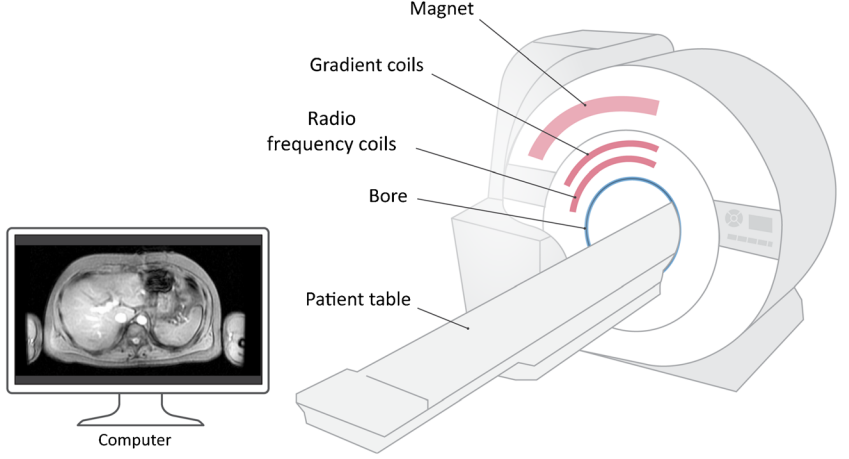
\includegraphics[width=\linewidth]{MRI-Schematic.png} 
 	\caption{Schematic of an MRI scanner taken from~\cite{Serai2021}.}
 	\label{fig:MRISchematic}
 \end{figure} 

\section{Magnetic Excitation and Relaxation Times}
Individual nuclei precess around the field $B_0$ at a
resonance frequency known as the Larmor frequency $\omega_0$ of the net magnetization vector, which generally occurs in the RF range of the electromagnetic spectrum and is related to the external magnetic field as:
\begin{equation} \label{eq:LarmorFrequency}
	\omega_0 = \gamma \cdot B_0,
\end{equation}
with $\gamma$ being the gyromagnetic ratio, which is a fixed value depending on the nuclei~\cite{SamplingStrategies}. When nuclei are placed in the presence of a strong static magnetic field such as $B_0$ the nuclei split into two energy states, either aligned parallel to the magnetic field $B_0$ (called a spin-up state) or aligned anti-parallel to $B_0$ (called a spin-down state). The spin-up state has a slightly lower energy level as compared to the spin-down state and is therefore preferred. This slight difference in the spin states ($0.001\%$) results in an overall net magnetization $M$ aligned in the same direction as $B_0$. To create an MR signal, the spins are excited out of their resting equilibrium, i.e. tipping $M$ away from $B_0$. To detect the signal from the hydrogen nuclei in the tissues an additional external field $B_1$ is introduced at the resonant Larmor frequency $\omega_0$ that can affect magnetization vector, causing it to rotate into a plane orthogonal to its original orientation. The rotated vector continues to precess around the $B_0$. The precession of the magnetization vector in the transverse plane can be detected by an RF coil tuned to the resonant frequency $\omega_0$. RF coils can be operated in a receive-only mode, in which case the inherent body coil is used as a transmitter; or the RF coils can be both transmit and receive. The purpose of the RF transmit coil is to create a time-varying $B_1$ field at right angles to $B_0$ that could be linearly or circularly polarized. The closer the receiving coil is to the source of the MR signal, the better the signal-to-noise ratio (SNR). Receiver coils generally comprise arrays of smaller individual coils or elements; however, each individual coil element has a limited depth penetration. Multiple arrays of coils, termed phased-array coils, can be used together to achieve a higher coverage. The multiple coils are electronically decoupled from one another so that they do not appear as just a single large coil. The images from individual coils are independently reconstructed and then grouped together to create the final image. An RF pulse of amplitude $B_1$, called excitation pulse, is applied for a certain time duration to tip the magnetization at an angle away from the $B_0$ field. The precessing transverse magnetization induces a voltage in the receiver RF coil; this induced voltage is known as the free induction decay. After the pulse, the magnetization returns to thermal equilibrium by processes known as MR relaxation. To fully encode the spatial information within the field of view (FOV), pulse sequences must be iterated numerous times. The time between successive iterations of a pulse sequence is known as the repetition time (TR). The time between the application of the initial RF pulse and the middle of the detected echo is known as the echo time (TE). Due to this the overall time to acquire an MR image is quite long~\cite{Serai2021}.\\
Once the RF pulse is turned off, $M$ continues to precess as it returns to its thermal equilibrium state. During this time, two types of relaxation occur: T1 (longitudinal or spin lattice) and T2 (transverse or spin/spin). One attribute that makes T1 and T2 so valuable for determining the signal in MRI is their sensitivity to the presence and type of tissue. It is this tissue dependence property that gives MR its excellent soft-tissue contrast. T1 relaxation describes the recovery of the longitudinal magnetization back to thermal equilibrium following a perturbation by an RF pulse. The longitudinal component regrows along the Z direction with a time constant T1. In other words, after the RF pulse is turned off, the protons that were disturbed give their energy to the surrounding environment and return back to their original equilibrium state, realigning with $B_0$. Hence T1 relaxation is also called longitudinal relaxation. Furthermore, because T1 relaxation involves the loss of energy that was put into the spin system by the RF pulse, it is also referred to as spin-lattice relaxation, the lattice consisting of surrounding macromolecules. This loss of energy is stimulated by the fluctuating magnetic fields associated with the dipole–dipole interactions of neighboring magnetic moments. T1 relaxation can only occur when these magnetic field fluctuations occur at the resonant frequency $\omega_0$. The rate at which the spin magnetization $M_z$ recovers to $M_0$ at time $t$ is called T1 relaxation time. It can be expressed as follows:
\begin{equation}
	M_z = M_0 \cdot \bigg(1 - e^{-\frac{t}{T1}} \bigg).
\end{equation}
A preferred method of measuring T1 relaxation is the Look-Locker method, which is based on the principle that one does not need to wait for the net magnetization vector to equilibrate in order to measure T1. Instead, an RF pulse is used with a small flip, which can be repeatedly applied. The acquisition pulse sequence is designed to generate a train of signals that gradually approaches a steady-state recovery. The recovery curve measured by this technique can be fitted to an exponential curve to provide an effective T1 measurement. This has become one of the most popular T1-mapping method for abdomen and cardiac imaging. The general principle of T1 mapping is to acquire multiple images with different T1 weightings and to fit the signal intensities of the images to the equation of T1 relaxation. T1 relaxation values for tissues can be estimated by fitting the data to the following equation:
\begin{equation}
	S = S_0 \cdot \bigg(1 - A \cdot e^{\frac{TI}{T1}} \bigg),
\end{equation}
where $S$ is the signal intensity measured at each inversion time value $TI$, $S_0$ is the initial signal intensity at time $t=0$ and $A$ is
a constant.\\
T2 relaxation results in the loss of transverse magnetization caused by interactions between the magnetic fields of neighboring hydrogen nuclei. It is not an energy loss process like T1 but is a loss of phase coherence within the spin system. This process, also known as spin-spin relaxation, leads to the destruction of transverse magnetization and causes the magnetic moments of the tissue to dephase. T2 mapping is a method of measuring the T2 value of the tissue. T2 relaxation time can be calculated using a T2 sequence with different echo times (TEs). The most fundamental sequence for T2 mapping is signal measured with spinecho techniques (multiple sequences with different TE values) [19]. Other 2-D sequences have been used, such as multi-echo spin echo (MSME) and fast spin echo (FSE) [19]. Synthetic MRI is another quantitative method in which a single saturation recovery turbo spin-echo sequence is used to estimate T2 transverse relaxation [20]. T2 relaxation values for tissues can be estimated by fitting the data to the following equation using a mono-exponential decay curve:
\begin{equation}
	S(TE) = S_0 \cdot e^{\frac{TI}{T2}},
\end{equation}
where $S(TE)$ is the signal intensity measured at each $TE$ and
$S_0$ is the initial signal intensity at time $t=0$.

\section{Image Acquisition and K-Space}
After discussing the physics behind MRI, it is time to look at the actual process of acquiring the image as well as the concept of the k-space.

\subsection{Image Acquisition}
Looking back at the Larmor frequency as defined in Equation~\ref{eq:LarmorFrequency}, the position of spins can be determined once they are brought into a magnetic field, which varies linearly across the object as seen in Figure~\ref{fig:1D_MRI_Measurement}. Their position is then be derived via frequency analysis of the measured MR signals, which is done using the Fourier transformation (FT). Generalizing this principle to 2D images is harder, however, as the simultaneous application of magnetic field gradients will render an unambiguous assignment only for spins aligned along the direction of the combined gradient. All spins orthogonal to this direction will be in the same field and thus yield identical Larmor frequencies. Thus, even with arbitrarily shaped magnetic field profiles, there will always be an infinite number of locations with identical field strength. A direct measurement of a 2D image from an intrinsically 1D signal is therefore not possible~\cite{SamplingStrategies}. %\\
The solution to this problem 
%of encoding a 2D image with an 1D MR signal 
is using time-variant magnetic fields. If the magnetic field at each point is varied in time, the location of spins can be established as long as the temporal variation is unambiguous for each position. 
%In principle, there are of course an infinite number of ways in which time-varying magnetic fields could be used to encode for each point in the image plane. 
A very powerful tool to design such imaging strategies is offered by the so-called k-space. %\\

\begin{figure}[h] %tpb
	\centering
	\graphicspath{{images/}{\main/images/}}
	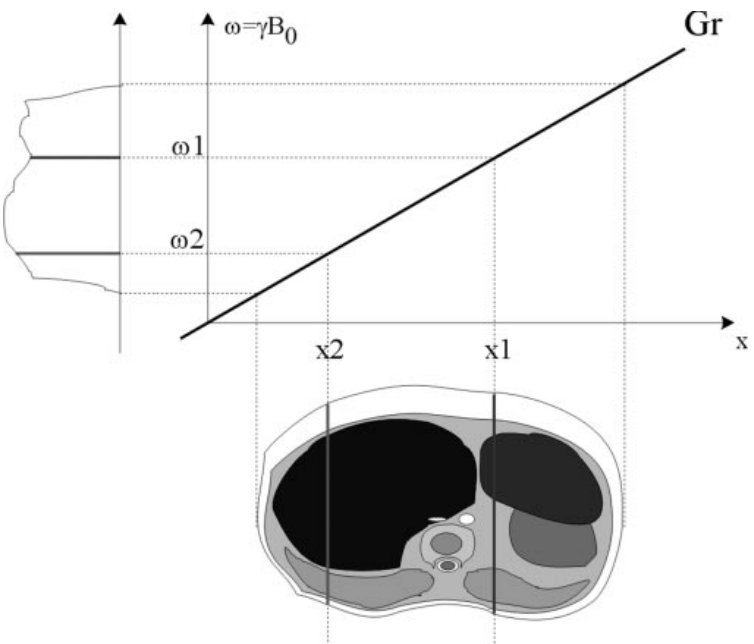
\includegraphics[width=0.75\linewidth]{1D_MRI_Measurement.png} 
	\caption{Schematic for the spatial encoding using a constant gradient adapted from~\cite{SamplingStrategies}. $G_r$ spins that are located at positions $x_1$ and $x_2$ have different Larmor frequencies $\omega_1$ and $\omega_2$. Spins located orthogonally to $Gr$ have the same x-coordinates and thus the same Larmor frequency}
	\label{fig:1D_MRI_Measurement}
\end{figure}


\subsection{K-Space}
The concept of the k-space is a generalization of the simple relation of a time-variant signal to a spectrum of two or more dimensions. An 2D image is related to a 2D k-space data set by a 2D FT, as seen in Figure~\ref{fig:2D_MRI_Measurement}
%, same as a 1D spectrum is related to the 1D signal by a normal (1D) FT. A 2D FT can be achieved by applying the (1D) FT successively row-by-row and column-by-column. 
As the FT is an information-preserving operation, the k-space data contains exactly the same information as the image data. Thus, in order to get the full image information, the full k-space data needs to be measured. The task of forming an image by this approach is then converted to the task of finding a way to measure the necessary corresponding k-space data. 
%An understanding of the physical meaning of the k-space domain can be derived from Figure~\ref{fig:1D_MRI_Measurement}. The time-domain signal defines the 1D k-space. Its coordinates are defined by the area under the gradient which the spins have experienced prior to the collection of each k-space data-point. 
Using the Larmor frequency again from Equation~\ref{eq:LarmorFrequency} the coordinates in 2D k-space will thus be given as $k_x = \gamma \cdot G_x \cdot t$ and $k_y = \gamma \cdot G_y \cdot t$. \\
In order to acquire an MR image, methods need to be developed 
%in order to get from one k-space point to the next. 
to traverse the k-space.
There are only two possibilities as seen in Figure~\ref{fig:kSpaceTrajectories}. The first one is to apply a gradient, in which case the k-space trajectory will be a line defined by the orientation of the gradient (see Figure~\ref{fig:constant_k-space_gradient}). As long as the gradient is kept constant, the k-space trajectory will be a straight line. 
%This way it is easy to see why simple superposition of two gradients will not produce an image. The resulting k-space trajectory will merely represent a straight line traversing k-space at some skewed angle. \\
The second method for traversing the k-space is the application of a refocusing pulse, which will lead to a jump of the k-space trajectory around the origin (see Figure~\ref{fig:refocusing_k-sapce_pulse}). It is clear that a spin-echo formation alone will not allow coverage of all of the k-space, since the trajectory would only jump between the two mirror symmetric points. A combination of spin echoes and gradients can, however, produce very efficient k-space trajectories. All of the existing k-space-based imaging techniques are based on some combination of these two basic means of traversing the k-space. \\
Is should be noted that the signals are measured 
%not continuously, but 
at discrete time intervals called the dwell-time of data acquisition. This discrete sampling leads to an ambiguous assignment of frequencies above a given threshold which is called the Nyquist frequency. The Nyquist frequency therefore determines the acquisition bandwidth inside which the signal should occur. The definition of the k-space coordinates implies that these are invariant with respect to the actual strength of the gradient used, as long as $G$ and $t$ are constant. Mathematically, data acquisition under a strong gradient and in a shorter acquisition time will yield the same k-space data and thus the same image as acquisition under a weaker gradient and a longer acquisition time. A shorter acquisition time and a closer spacing of sampling points are equivalent to a higher-acquisition bandwidth. Since the received noise grows with the square root of the bandwidth, a faster imaging technique will therefore by principle always carry the penalty of a lower signal-to-noise ratio (SNR)
%, even if all other factors influencing high-speed imaging are neglected. \\
For a conventional spin-echo imaging sequence
%, which is still widely used, 
a typical acquisition time of 5 to 10~ms for each phase-encoding step is used. Acquisition of 
%typically 
192 to 256 phase-encoding steps therefore requires a total net acquisition time of 1 to 2~s. However, this is much shorter than the 
%total 
actual
acquisition time of such a sequence, which is determined by the repetition time defined by the T1-contrast. 
%From the aforementioned general considerations 
It 
%immediately 
follows that the SNR of a fast imaging sequence leading to acquisition times of approximately 50~ms, will be lowered by at least a factor of 5 to 10, regardless of the actual sequence used. 
%Fast imaging therefore requires improved SNR provided by radio-frequency coil designs. The improvement in SNR driven by the need for fast imaging will also benefit slower techniques, providing images with better spatial resolution and/or higher SNR. 
Fast imaging thus relies on radio-frequency coil designs improving the SNR.\\
The discrete data sampling has some additional consequences regarding the sampling density and coverage of data in k-space. Different parts of the k-space encode different features of the image: The center of the k-space hold the lower frequencies which represent the image contrast, whereas the outer parts encode the higher frequencies for sharp structures. Due to the symmetry of the 2D FT, this statement can also be reversed: The image center will be encoded by low-resolution k-space data. Therefore, sampling of sparsely distributed k-space data will reduce the effective field of view of the final image. \\
Mathematically, the final image will look exactly the same, irrespective of the way the data is sampled in the k-space. In practice, however, different approaches 
%to sampling 
can have a major impact on image quality
%. This is due to the fact that sampling 
as the data has to 
%proceed 
sampled
sequentially. The observed spins evolve not only as a function of the gradients defining the intended k-space trajectory, but are also influenced by other mechanisms unrelated to image encoding. It is noteworthy that the coordinates in k-space are expressed in units of a phase angle across space. Any mechanism affecting the phase of the signal along this trajectory will therefore alter the k-space trajectory. Some such commonly occurring mechanisms are flow and motion effects, magnetic field inhomogeneities, as well as susceptibility and chemical shift effects. The consequence of such phase effects in terms of imaging properties is dependent on the particular sequence and data sampling speed. In addition to phase effects, the signal decay with T2 needs to be taken into account also, especially if the data acquisition time is similar or even longer than the T2 of the observed tissues under construction~\cite{SamplingStrategies}.

\begin{figure}[h] %tpb
	\centering
	\graphicspath{{images/}{\main/images/}}
	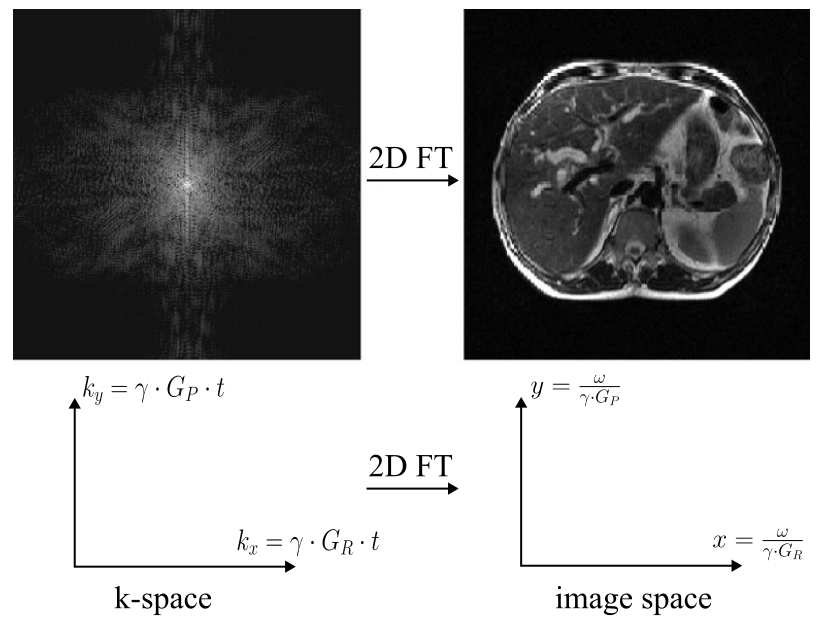
\includegraphics[width=0.75\linewidth]{2D_MRI_Measurement.png} 
	\caption{Correspondence of the image domain and the k-space via a 2D FT, adapted from~\cite{SamplingStrategies}. The coordinates of each domain are defined by the Larmor frequency according to Equation~\ref{eq:LarmorFrequency}.}
	\label{fig:2D_MRI_Measurement}
\end{figure}

\begin{figure}[h] %tpb
	\centering
	\graphicspath{{images/}{\main/images/}}
	\begin{subfigure}{0.445\textwidth}
    		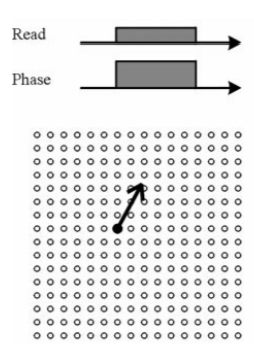
\includegraphics[width=\textwidth]{constant_k-space_gradient.png}
    		\caption{Schematic of a constant gradient creating a straight k-space trajectory.}
    		\label{fig:constant_k-space_gradient}
	\end{subfigure}
	\hfill
	\begin{subfigure}{0.445\textwidth}
    		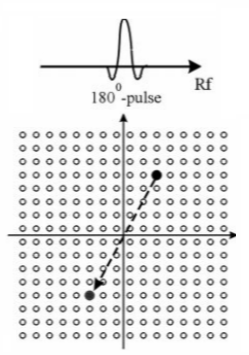
\includegraphics[width=\textwidth]{refocusing_k-sapce_pulse.png}
    		\caption{Schematic of an refocusing pulse inverting the phase of the k-space.}
    		\label{fig:refocusing_k-sapce_pulse}
	\end{subfigure}
	\caption{Methods of moving in the k-space using a) constant gradients to move along straight lines or b) mirror the k-space at the origin using a refocusing pulse. Adapted from~\cite{SamplingStrategies}.}
	\label{fig:kSpaceTrajectories}
\end{figure}

\subsection{Rectilinear K-Space Sampling}
Almost all MR imaging sequences 
%used in clinical routine presently 
are based on rectilinear k-space sampling, i. e., the sampling points 
%in k-space 
are placed on a rectangular grid. This 
%reflects the ability to use a 
allows the usage of the fast Fourier transform (FFT) 
%for such a sampling strategy. It allows 
which enables 
image reconstruction in 
%considerably under 1~s
a very short time (under 1~s). 
%With special reconstruction processors, the reconstruction speed can be as high as 10 to 25 images per second. 
For comparison, using
the 
%general 
2D FT 
to transform a non-rectilinear grid can take about
%for transformation of a comparable number of non-rectilinear grid points in comparison requires
5 to 50~min per image~\cite{SamplingStrategies}.
%, using identical computer hardware. \\
Utilizing the two means of traversing the k-space, 
%the basic techniques for 
rectilinear sampling can be divided into spin-echo-based techniques and gradient-echo-based techniques. In all rectilinear sampling techniques, the gradient which is used during signal acquisition is commonly called the readout gradient, whereas gradients used to bring the k-space trajectory to a certain starting point before data acquisition are called phase-encoding gradients. \\
A gradient echo is formed using a reversal of the readout gradient. In conventional gradient-echo imaging, only the refocusing part of the k-space trajectory is measured, whereas the signal dephasing as well as phase encoding is performed prior to data acquisition (Fig. 8). The experiment is repeated after the recovery time TR, using different offsets of the phase-encoding gradient prior to each acquisition step. Using the k-space, it can be easily seen how gradient-echo imaging can be generalized to a faster technique, using less excitation periods by sampling more than one k-space line after each excitation. Repeating gradient reversal and the application of a phase-encoding gradient can be used to read out several k-lines per acquisition with a concordant reduction in total imaging time. In the extreme case, all k-space data can be read out following a single excitation. This is called the single-shot, echo-planar imaging (EPI) sequence~\cite{EPI}. \\
%Historically, the development took place the other way round: EPI was first invented by P. Mansfield, and gradient echoes followed several years later. The concept of the k-space was not widely known at that time, therefore, the intrinsic relationship between the two techniques has only been acknowledged gradually. 
Despite the close conceptional similarity between EPI and gradient echo techniques 
%with respect to their k-space trajectories
, both types of sequences have vastly different imaging and hardware implications. This difference is caused by the sequential sampling of k-space points and the resulting influences on the signal of the mechanisms mentioned previously. As the signal decays with T2 the signal amplitude is reduced during data acquisition. For conventional gradient-echo imaging, even with moderate gradient strength (and thus longer acquisition times), this effect is inconsequential since the typical acquisition times of 5 to 10~ms are considerably shorter than the typical T2 of tissues. For EPI, however, the total acquisition time for n k-space lines is n times longer, even if the time necessary for gradient reversal and phase encoding is neglected. For the moderate acquisition times noted previously, this will lead to total acquisition times of 1~s or more, which exceeds most T2 values observed in human tissues. 
%Dephasing of spins across the selected slice will lead to T2 of the order of 100~ms at most. 
For identical acquisition times, as in our gradient-echo example, the signal will have vanished long before the end of data acquisition leading to information loss. 
%Depending on whether data acquisition has commenced at the center or in the outskirts of k-space, the resulting image will either be severely blurred or reveal merely contours without contrast. This illustrates that 
Thus EPI 
%absolutely 
requires very fast data acquisition in order to 
%acquire 
scan all of the k-space data within 
%not much more than 100~ms at most; otherwise, 
100~ms or else image quality will deteriorate significantly. In the given time range, state-of-the-art scanners can acquire 64 to 128 phase-encoding steps. Longer acquisition times allowing for higher 
%nominal 
resolution are of course technically feasible, but the T2-decay 
%of the signal will 
prohibits the realization of this 
%nominal 
resolution. 
%Since cerebral spinal fluid (CSF) has a long T2, EPI images of the head with long acquisition times can look deceptively sharp. It must be noted, however, that the perceived sharpness applies only to CSF-filled structures, whereas the true resolution of parenchyma with a T2 of approximately 60~ms is considerably worse. 
With even stronger and faster gradients it is 
%of course feasible 
possible to acquire true high-resolution images with short acquisition times, but the penalty in SNR for such applications is too severe and has prohibited its use for most forms of morphological imaging. The EPI technique has emerged, however, as an ideal vehicle for functional imaging either in BOLD-based fMRI, in first-pass perfusion measurements or in diffusion imaging, but it is not a viable technique for high-resolution morphological imaging~\cite{SamplingStrategies}.\\
Even for short acquisition times, EPI suffers from severe problems regarding its imaging properties, which are caused by the phase-altering mechanisms mentioned previously. Chemical shift effects and susceptibility both lead to signal phase shifts which increase linearly with time. Since data acquisition along the readout gradient is fast, there is little effect in the readout direction. In the phase-encoding direction, however, the dwell time amounts to the acquisition time of one k-space line. 
%For the acquisition of 64 k-space lines in 64~ms, the field of view in frequency units will be 1000~Hz. For a frequency shift of fat vs water of approximately 200~Hz at 1.5~T, this will mean that the signal of fatty tissue will be shifted by 20$\%$ of the image width. The resulting misregistration artifact necessitates the use of fat suppression for practically all EPI applications. 
Field inhomogeneity and susceptibility will lead to a similar shift. Since the resulting frequency shifts are not as discrete as chemical shift effects, the misregistration will vary continuously leading to highly non-linear image deformations. An additional problem in EPI relates to the fact that the k-space trajectory runs in opposite directions in every other k-space line due to the alternating polarity of the readout gradient. Any asymmetry in the acquired data will therefore lead to some slight perturbation in any other line known as the $180°$ artifact.  
%The final image will therefore be a superposition of the true image with an image representing the perturbation in every other k-space line. From this discussion of the k-space trajectory, it is easy to see that this perturbation will generate an image which is displaced by half the field of view in the phase-encoding direction. This is the so-called $180°$ artifact.
\\All the confounding factors discussed will produce such artifact. With appropriate post-processing routines based on reference signals, some of the sources of artifacts can be corrected for. In general, the $180°$ ghost will become stronger whenever any of the mechanisms mentioned previously become significant and will therefore deteriorate the image quality further. Motion can also cause phase-effects on the signal. With an alternating readout gradient, motion along this direction will be refocused in every even refocusing period. Consequently, a flow-dependent $180°$ ghost will occur. Motion along the phase-encoding direction will lead to a velocity-dependent increase in the signal phase and consequently to a velocity-dependent signal displacement. 
%Signal from a round vessel with laminar flow will therefore appear as a boomerang-shaped artifact displaced from the vessel wall. Any vascular diagnosis based on EPI images therefore has to be made with the utmost care. The inherent artifact behavior limits the practical use of EPI to examinations of the head. Abdominal or thoracic EPI and even cardiac EPI have not been developed beyond a feasibility state. They require considerable efforts in region-selective shimming and even post-processing, using actual field maps of the patient such that the time advantage of EPI is lost. 
Thus, for the time being, EPI 
%therefore has to be
is regarded as a brain-only technique 
%where it serves as a vehicle for the 
for fMRI applications, including diffusion and perfusion imaging~\cite{SamplingStrategies}.\\
Conventional gradient-echo imaging suffers from no such effects and can therefore be applied all over the body with no or only mild susceptibility misregistration. Chemical shift effects will, however, influence the contrast of gradient-echo images by the chemical-shift-dependent dephasing of fat and water signals. Signals from fat and water protons located at the same position will periodically be in- and out of phase with each other in a time interval determined by their difference in Larmor frequencies. 
%For 1.5~T the time difference between the two extreme conditions will be approximately 2.5~ms. Images acquired with TEs differing by 2.5~ms will look dramatically different due to this effect, although T2-dependent effects for such small TE differences will be negligible. 
As shown in Fig. 11, the out-of phase image will show a considerable reduction in signal amplitude in tissues containing both fat and water protons such as bone marrow. In addition, an artificial black line will appear at the interface between fatty and water tissues due to the zero crossing of the signal between these antiphasic images. When (im)properly used, this artifact can be used to beautify images, giving them a crisp and well-defined appearance. Care must be taken, however, not to mis-read this artifact as an anatomical structure. With respect to the total acquisition time, gradient-echo imaging is somewhat slower than EPI due to the necessity of repetitive application of excitation pulses. Gradient-echo sequences, which are optimized for speed, typically achieve imaging times of 200 to 400~ms, using gradient systems comparable to those of EPI. Due to the strong signal saturation caused by the very short repetition times, the intrinsic SNR is comparably low. \\
%(but for many applications still satisfactory). 
%The SNR can be optimized by using low-excitation flip angles and/or total signal refocusing (true FISP). In combination with bolus application of contrast agent, gradient-echo sequences allow the acquisition of MR angiograms especially of the thorax, abdomen, and the extremities with unprecedented image quality. This  relatively new application has led to whole new field of applications for gradient-echo imaging. \\
In order to reach a compromise between the more efficient sampling of EPI and the much more benign artifact behavior of gradient echoes, 
%segmented 
mixed approaches have been developed. In these approaches, more than one excitation is used and several k-lines are sampled per excitation. 
%Depending more on the perspective of their creators than on anything else, such approaches are called multi-echo gradient echo, multi-shot EPI, or segmented EPI. 
The optimum number of k-lines per excitation is strongly dependent on the particular application
%; it 
and can range from 3 for MR angiography and cardiac imaging to 64 or more for high-resolution head imaging.

\subsection{Spin-Echo Techniques}
In spin-echo techniques, refocusing pulses are used in the construction of the k-space trajectory. Conventional spin-echo techniques acquiring one k-line per excitation are identical to gradient-echo techniques with respect to the k-space sampling strategy used. In rapid acquisition relation enhanced imaging (RARE, e. g., turbo spin echo and fast spin echo), multiple refocusing pulses are employed in order to sample more than one and, in the extreme case, all k-lines per excitation [15]. In order to suppress unwanted coherences, the k-space trajectory in RARE has to be brought to the identical position at the time of application of each refocusing pulse. This is achieved by using a phase-encoding rewinder after reading out each k-line (Fig. 12). Conceptionally, RARE is very similar to EPI, however,
%and the possibility to build a spin-echo-based technique has already been mentioned in the original paper by Mansfield. 
The spin-echo refocusing makes a huge difference with respect to the artifact behavior. For once it should be noted that the direction of data sampling is identical for all k-lines. Therefore, no $180°$ ghosts will occur. In addition, all phase changes caused by chemical shift, susceptibility, etc., are refocused. The phase effects therefore do not accumulate but re-start in each k-line just like in conventional spin-echo sequences. Motion effects are in principle similar to the ones discussed for EPI with a refocusing of flow in every even echo. Since for low flow the resulting $180°$ effect will be weak, and for high-flow velocity the signal will vanish from the image due to outflow during the echo train, the resulting flow artifact behavior of RARE is very benign. 
%Slow-flow vessels (e. g. liver veins), which are black on conventional spin-echo imaging, appear very bright on T2-weighted RARE imaging due to this even echo refocusing effect.
The insensitivity to other mechanisms leads to T1 and T2 as the basic contrast mechanism for RARE. From the discussion of the properties of k-space it follows that the T2-contrast is determined by the echo times of the acquisition of the k-lines with low phase encoding. The T2-contrast of a given implementation can thus be varied widely by changing the order of the phase-encoding gradient. By similar consideration, T2-relaxation along the echo train leads to a loss of resolution when the k-lines carrying the edge information are acquired at long echo times. For most diagnostic applications in high-resolution imaging, a segmented acquisition is therefore preferred with echo train lengths ranging between 8 and 35 for T2-weighted scans and 3 to 5 for T1-weighted scans. Nevertheless, single-shot variants are also being used~\cite{SamplingStrategies}. 
%Especially single-shot RARE (or single-shot FSE) with very strong T2-contrast has been shown to be extremely useful for imaging of liquid-filled structures like in MR myelography [16], MR urography [17], or MR cholangio-pancreatography (MRCP) [18]. 
Using half-Fourier phase encoding in half-Fourier acquired single-shot turbo spin echo (HASTE) [19], single-shot implementations with less T2-contrast are also feasible. It has been noted that signal from fat is significantly brighter in RARE compared with conventional spin-echo imaging at equal echo times [20]. This is due to so-called J coupling of protons in lipids, which leads to a periodic modulation of their resonances just like the modulations caused by two elastically coupled pendulums [21]. This modulation will not be refocused but continue despite the reversal of the phase by the 180 pulse (Fig. 13). At a time interval equal to 1/(2 J), the signals from such coupled spins will be opposed and therefore canceled. For typical coupling constants, this condition is reached at echo times of 80 to 140 ms typically used for T2-weighted imaging. The multiple refocusing in an echo train ensures that the phase of the signals from coupled spins stay together along the echo train; thereby, signal suppression is avoided and fat will appear bright. A similar cause is implied for a relative reduction in susceptibility contrast on RARE images (Fig. 14). Static susceptibility effect will be refocused on both spin-echo sequences. If spins move along strong local gradients as caused by hemorrhage, for example, the motion-dependent variation of their Larmor frequency cannot be refocused due to the random nature of the motion. Multiple refocusing pulses, however, will ensure that the spin phases stay together. Some such diffusion-dependent dynamic susceptibility effect is observed in most organs (nuclei in the brain and basal ganglia, liver, lung, etc.). Therefore, RARE images can look very different from conventional spin-echo images at identical echo times. Due to the repetitive use of refocusing pulses and the necessity for rewinding the phase-encoding gradient, RARE is inherently slower than EPI. The gradient performance of current scanners allows refocusing intervals as short as 4 ms or less. The high radio-frequency power inherent to a long train of $180°$ pulses limits, however, the range of applications for such fast echo trains. Even though this problem can be ameliorated by the use of lower refocusing flip angles, EPI with typical readout times of 1 ms or less will remain faster. The big advantage of spin-echo techniques remains, however, their lack of distorting artifacts which makes spin-echo techniques applicable all over the body. Even high-quality cardiac images with HASTE have been demonstrated as well as perfusion and ventilation imaging of the lung [22].

\subsection{Non-Rectilinear K-Space Sampling}
A common problem of all rectilinear sampling techniques is the very heterogeneous nature of the k-space trajectories used: Data are acquired along straight k-space lines under a constant gradient. Going around the corner of the trajectory requires very fast switching for a brief period. The combination of both modes of operation is very demanding on the gradient power amplifiers, which have to be able to alternate between the two modes. A more common load on the gradients is offered by the use of curved k-space trajectories. Especially spiral trajectories [23, 24] have won considerable interest due to their very efficient use of the gradient system (Fig. 15). For a given gradient system it is also possible to calculate the trajectory achieved by running the gradient system always under full load. In terms of the gradient performance, spirals therefore are considerably more efficient than rectilinear k-space trajectories. A practical problem relates to image reconstruction which requires algorithms not (yet) commonly available and which can take several seconds per image on a typical scanner. In order to make use of the very fast FFT algorithm, the typical approach to reconstruction of data sets acquired with spiral (or other non-rectilinear) trajectories is to first interpolate the data onto a rectilinear grid and then to use FFT for the reconstruction itself. With further developments of spirals, it is expected that reconstruction algorithms will become widely available. The ultimate success of spiral imaging will then be determined by its inherent imaging properties, which are significantly different from rectilinear scans. Firstly, it should be noted that spirals do not have a preferred orientation like the readout- and phase-encoding direction in rectilinear scans. Constant off-resonance effects, such as chemical shift, field inhomogeneity, and susceptibility, will therefore not lead to a displacement in the phase-encoding direction. It will instead lead to blurring of the corresponding structures [25]. In some respects this can be regarded as an advantage since the severe distortions of EPI images are avoided. On the other hand, some mild distortion in EPI images can be tolerable for most applications, whereas blurring artifacts are not. These artifacts can be avoided if the off-resonance frequency is known. The data can then be corrected and a sharp image will be produced. Consequently, for most applications of spiral imaging a field map is acquired prior to the scan in order to measure the local off-resonance effects. Another problem of spiral imaging is the fact that severe artifacts can arise when the k-space trajectory produced by the gradient system is not exactly identical to the trajectory used for image reconstruction. It is thus necessary to accurately calibrate the gradient system or to even measure the actual trajectory used. Especially spiral images in tilted orientations involving all gradients simultaneously sets very high requirements for the gradient switching behavior. A favorable property of spirals is the motion correction inherent to the trajectory [26]. The periodic nature of spirals ensures that part of the data are motion corrected. For the remainder, motion-dependent dephasing will be mild. Consequently, spirals have been demonstrated to yield good image quality for moving structures like blood in vessels or even the heart. It is noted that EPI also has an inherent motion correction in every even refocusing period, as discussed previously. The interleaved nature of motion-corrected and motion sensitized k-lines leads, however, to a 180 artifact, whereas in spirals the distribution of motion-corrected and motion-sensitized data is continuous and therefore no artifacts are formed. Apart from spirals, other non-rectilinear k-space trajectories have been suggested. Back projection uses a star-like trajectory and was in fact the method used by Lauterbur [27] in his first demonstration of MR imaging. Back projection allows the realization of extremely short echo times and has therefore found applications especially for imaging of solid structures. Its inhomogeneous k-space coverage with a high sampling density for points at the center of k-space and its somewhat awkward artifact behavior have limited its success for conventional imaging. Other trajectories, such as rosettes or even random k-space trajectories [28], have also been explored. A common feature of all non-rectilinear trajectories relates to their non-periodic nature, which produces severe artifacts when the field of view of the data acquisition is less than the size of the object. For rectilinear scans this leads to severe fold-over artifact, which can be tolerated as long as it does not affect relevant structures or even is totally avoided when it occurs in the readout direction, where oversampling can be applied without penalty in the data acquisition time. For non-rectilinear scans oversampling is not an option, since the field of view is determined by the distance between adjacent parts of the trajectory, rather than by the sampling rate along the trajectory. Oversampling therefore requires a denser k-space trajectory with concordant prolongation of the acquisition time. For an insufficient field of view of the k-space data, misregistration artifacts can be very severe, depending on the trajectory used. Spirals produce a circular rim artifact around the image. It is therefore mandatory to ensure that the k-space trajectory is sufficiently dense to always cover the whole object of interest. This limitation is especially severe for cardiac imaging, where the size of the field of view of a short axis plane can be considerable. Limitation of the field of view by the use of surface coils with limited sensitivity range is therefore mandatory for many applications of non-rectilinear trajectories.

\section{Imaging Acceleration}
To alleviate the slow image acquisition times of the MR imaging, different MRI acceleration techniques are used. Most of these included scanning less k-space lines during signal acquisition, omitting certain frequencies
%higher frequencies and fully scanning the center region. 
The amount of k-space lines that are omitted are usually given by a reduction factor $R$. While there are different subsampling techniques, most involve fully sampling a center region containing the lower frequencies and dropping higher frequencies, which are deemed less important. However, all of these methods create artifacts like image blur during image reconstruction leading to different technologies being developed to minimize these effects such as compressed sensing (CS) and parallel imaging (PI).

\subsection{Compressed Sensing}
When looking at a subsampled k-space one can approach the reconstruction of the MR image as an problem of an under-determined system. This can then be solved using compressed sensing techniques.

\subsection{Parallel Imaging}
Parallel imaging is another popular technique for multi-coil data as it allows for merging different images reconstructed from each coil to get an averaged image that includes all regions of the image in good quality.

\section{Motion-Corrected Reconstruction} \label{Sec:Motion-CorrectedReconstruction}
Patient motion during acquisition is one of the major impediments of high-quality MRI scans. This is especially true for thoracic and abdominal imaging, as organs move during breathing. This motion can induce several consequences on MR signal formation. Intraview and interview motion have to be distinguished between: motion is intraview when occurring during individual MR experiments (between RF excitation and echo formation), whereas motion is interview when occurring between individual MR experiments. Whenever the period of motion is slow compared to the period of MR acquisition defined by the repetition time $TR$, the assumption can be made that motion is interview. This is often a reasonable assumption when considering pseudo-periodic motion induced by respiration, and also possibly by cardiac contraction, which are the two common sources of motion in cardiac and abdominal imaging (typically, the adult respiratory period is about 4–5 $s$, and $TR \approx 10 ms$ for fast imaging). Interview motion results in spatial encoding inconsistencies, and thus in image deterioration which can take complex forms (blurring/ghosting artifacts) as acquisition is performed in a Fourier space. Several strategies can be employed in order to handle patient motion better. Patient cooperation is the most commonly used method. However, breath-holds cannot last much longer than $20 s$ and physiological drifts cannot be completely avoided. This leads to a limitation on the time-period of signal recording and thus, signal-to-noise ratio (SNR). Moreover, the position of organs in successive breath-holds may not be reproducible. Synchronization techniques are well-established and systematically used in clinical protocols, but they require a high-level of motion reproducibility. This is often a limiting factor considering heart rate variability (whether in free breathing or during a breathhold), and respiratory variability in terms of amplitude and frequency. This is why alternative techniques have been put forward with the aim of inverting the process of spatial encoding of moving structures that underlies artifacts. While it is possible to correct for motion prospectively, by modulating the magnetic field gradients and RF fields in order to cancel the effect of motion in the Bloch equations, the method is limited to correcting of, at best, affine motion, due to magnetic field gradient systems being linear. Motion can also be compensated for in reconstruction, however, many methods are restricted to rigid or affine motion due either to computational issues or to the difficulty of modeling complex displacement fields~\cite{GRICS}. The latter however seems to become less of a problem as image registration improves with e.g. the help of deep learning.\\
Motion-resolved data acquisition for these applications are usually accelerated by Parallel Imaging or Compressed Sensing techniques yielding sub-Nyquist sampled (subsampled) k-space data. In order to reconstruct aliasing-free images, these methods rely on reconstruction schemes that, for example incorporate sparsity or low-rank constraints to solve the ill-posed problem. Fixed sparsity assumptions in Compressed Sensing are often too restrictive and incapable of fully modeling spatio-temporal dynamics. Careful fine-tuning between regularization and data consistency is required and especially in highly subsampled cases residual aliasing may remain in the image (under-regularization) or staircasing and blurring artifacts can occur (over-regularization) which affect the image registration. After reconstruction, non-rigid motion fields can be estimated in image space from reconstructed images by solving a registration problem. A particular interest and challenge lies in the derivation of reliable motion fields which capture the spatio-temporal non-rigid deformations, such as respiratory or cardiac movement. Instead of performing these two steps sequentially, motion-compensated image reconstruction schemes like \emph{GRICS}~\cite{GRICS} integrate both motion field estimation and motion correction into the reconstruction process. These methods require reliable motion-resolved images from which the motion fields can be estimated. Motion field estimation can be controlled or supported by external motion surrogate signals, initial motion field estimates, from motion-aliased images or low-frequency image contents. Moreover, spatio-temporal redundancies can be exploited to achieve an aliasing-free image. While these methods have been proven to be more robust against registration errors, they can require a significantly increased computational demand and/or limit imaging acceleration~\cite{Kuestner2022}.

There are also approaches for learning new subsampling strategies in a data-driven manner (pruning unimportant k-space frequencies)~\cite{MRISubsamplingPruning} as well as deep learning based radial~\cite{DeepMRIReconstructionRadialSubsampling} and non-Cartesian~\cite{DeepMRIReconstructionSubsampling} subsampling for MRI acceleration.

\chapter{Image Transformations and Registration} \label{Ch:ImageTransformationsAndRegistration}
In this chapter a brief overview over the different kinds of image transformations is given, followed by a deep dice into the challenges of image registration.

\section{Image Transformations}
There are two major groups of image transformations: linear and non-rigid.

\subsection{Linear Transformations}
Linear Transformations are a common group of global transformation, which include rotation, scaling and translation. As these are global operations, one can express them as matrix operations. If a 2D point has the cartesian coordinates $\mathbf{p} = [x,y]^T$ it can be extended to 3D as $\mathbf{p} = [x,y,1]^T$ instead of being only 2D. This allows for combining all of the linear transformations into a single matrix:
\begin{align}
	\begin{bmatrix}
		x'\\
		y'\\
		1
	\end{bmatrix} 
	&= 
	\begin{bmatrix}
		\cos(\theta) & -\sin(\theta) & 0\\
		\sin(\theta) & \cos(\theta) & 0\\
		0 & 0 & 1
	\end{bmatrix}
	\cdot 
	\begin{bmatrix}
		s & 0 & 0\\
		0 & s & 0\\
		0 & 0 & 1
	\end{bmatrix}
	\cdot 
	\begin{bmatrix}
		1 & 0 & t_x\\
		0 & 1 & t_y\\
		0 & 0 & 1
	\end{bmatrix}
	\cdot
	\begin{bmatrix}
		x\\
		y\\
		1
	\end{bmatrix}
	\\
	&=
	\begin{bmatrix}
		s \cdot \cos(\theta) & -s \cdot \sin(\theta) & t_x\\
		s \cdot \sin(\theta) & s \cdot \cos(\theta) & t_y\\
		0 & 0 & 1
	\end{bmatrix}
	\cdot
	\begin{bmatrix}
		x\\
		y\\
		1
	\end{bmatrix}
\end{align}
with $\theta$ being the angle of the rotation, $s$ the scaling factor as well as $t_x$ and $t_y$ being the translations in x- and y-direction. This can be further generalized as a linear matrix multiplication:
\begin{equation}
	\mathbf{p'} =	
	\begin{bmatrix}
		x'\\
		y'\\
		1
	\end{bmatrix} 
	= 
	\begin{bmatrix}
		a_{11} & a_{12} & a_{13}\\
		a_{21} & a_{22} & a_{23}\\
		0 & 0 & 1
	\end{bmatrix}
	\cdot
	\begin{bmatrix}
		x\\
		y\\
		1
	\end{bmatrix}
	 = \mathbf{A} \cdot \mathbf{p}
\end{equation}
where $\mathbf{A}$ is the general affine transformation matrix.


\subsection{Non-Rigid Transformations}
The second category of transformations allow elastic or non-rigid transformations. These transformations are capable of locally warping the image. Non-rigid transformations include radial basis functions, physical continuum models, and large deformation models like diffeomorphisms.


\section{Image Registration} \label{Sec:ImageRegistration}
Image registration is a challenging, yet important task for image processing. It can be described as the process of transforming different image datasets into one coordinate system with matched imaging contents~\cite{Haskins2020}. In the medical field this can be used for clinical applications such as disease diagnosis and monitoring, image-guided treatment delivery, and post-operative assessment. Medical image registration is typically used to pre-process data for tasks like object detection (for e.g. tumor growth monitoring) and segmentation (for e.g. organ atlas creation) where variation in spatial resolution is common between modalities like CT and MRI and patients. Thus the performance of these methods is dependent on the quality of image registration~\cite{Chen2020}. \\
Medical image registration was often done manually by clinicians, however, registration tasks are often challenging and the quality of manual alignments is dependent on the expertise of the user. These manual registrations are thus not only time consuming, but also hardly reproducible leading to high interobserver-variability. The need for automatic registration is very much apparent, but this task remained hard to solve for a long time, requiring a lot of computational power and time for computer algorithms to solve the problem. While neural networks also require a lot of computational power and time to train, they promise fast execution after training. With the rise of deep learning these network gained popularity and now pose a real alternative to conventional algorithms and manual registration~\cite{Haskins2020}. We will discuss these new approaches in the next section, but first we need to formally define our problem.\\
In pair-wise image registration two images ($F$ and $M$) are to be aligned, with $F$ denoting the fixed and $M$ the moving image. T is the desired spatial transformation that aligns the two images. This can be posed as an optimization problem:
\begin{equation}
	T' = \arg\max S(F, T(M)),
\end{equation}
with $T'$ being the best transformation that maximizes the similarity $S$ between the two images. This process is done iteratively improving estimates for the desired T, such that the defined similarity in the cost function is maximized~\cite{Chen2020}.\\
Transformations can be categorized as rigid, affine, and deformable. A rigid transformation consists of rotation and translation; an affine transformation
includes translations, rotations, scaling, and sheering; the two kinds of transformations are described as a 2D single matrix. Unlike rigid and affine transformation, deformable transformation is a high-dimension problem that we need to formulate by a 3D matrix for 2D deformable registration i.e., a so-called deformation field. While rigid and affine registration algorithms have already achieved good performance in many applications, deformable registration is still a challenging task due to its intrinsic complexity, particularly when the deformation is large. However, these are also the transformations most likely encountered in clinical practice as it can be utilized to fuse information from different modalities such as MRI and CT~\cite{Zou2022}. Additionally, deformable image registration can also be
utilized for various computer-assisted interventions like biopsy~\cite{Tam2016} and (MRI-guided) radiotherapy~\cite{Chen2017, Rigaud2019}. \\
Intuitively, deformable image registration is an ill-posed problem, making it fundamentally different from other computer vision tasks such as object localization, segmentation or classification. Given two images, deformable image registration aims to find a spatial transformation that warps the moving image to match the fixed image as closely as possible. However, there is no ground-truth available for the desired deformation field and without enforcing any constraints on the properties of the spatial transformation, the resulting cost function is ill-conditioned and highly non-convex. In order to address the latter and ensure tractability, all image registration algorithms regularize the estimated deformation field, based on some prior assumptions on the properties of the underlying unknown deformation~\cite{Chen2020}.\\
Many methods have been proposed for medical image registration to deal with the complex challenges of this task. Popular conventional registration methods include optical flow~\cite{Yang2008}, demons~\cite{Vercauteren2009} and many more. However, most of these still lack accuracy and computation speed, which makes newer deep learning approaches all the more interesting~\cite{Fu2020}.

\chapter{Deep Learning}
Deep learning, and neural networks in general, have seen a significant rise in usage over the last couple of years due to many breakthroughs in areas of image recognition, segmentation and also registration. After a brief overview of different neural network architectures that can be used for, among other applications, image registration, a comprehensive guide for the specifics of such an training process is given including different training methods and evaluation metrics.

\section{Deep Learning Architectures} \label{Sec:DeepLearningArchitectures}
Neural networks, despite the theoretical concepts being around for decades, have seen a meteoric rise in popularity over the last few years as constraints on computational power have been alleviated. Especially deep neural networks, which are often summarized under the term deep learning (DL). Recent years have witnessed an almost exponential growth in the development and use of DL algorithms, sustained thus far by rapid improvements in computational hardware (e.g. GPUs). Consequently, clinical applications requiring image classification, segmentation, registration, or object detection/localization, have witnessed significant improvements in algorithmic performance, in terms of accuracy and/or efficiency~\cite{Chen2020}. The following network architecture are widely used for different tasks including medical image registration. \\
Some basic stuff about network training, testing and different architectures that are relevant for the later Chapters.

\subsection{Convolutional Neural Networks} \label{SubSec:CNNs}
Convolutional neural networks (CNNs) are a type of deep neural networks with regularized multilayer perceptron, which are mainly used for image processing. CNNs use convolution operations instead of general matrix multiplications in typical neural networks. These convolutional filters make CNNs very suitable for visual signal processing. Because of their excellent feature extraction ability, CNNs are some of the most successful models for image analysis. Different variants of CNN have been proposed and have achieved the-state-of-art performances in various image processing tasks. A typical CNN usually consists of multiple convolutional layers, max pooling layers, batch normalization layers, sometimes dropout layers, a sigmoid or softmax layer. In each convolutional layer, multiple channels of feature maps are extracted by sliding trainable convolutional kernels across the input feature maps. Hierarchical features with high-level abstraction are extracted using multiple convolutional layers. These feature maps usually go through multiple fully connected layer before reaching the final decision layer. Max pooling layers are often used to reduce the image sizes and to promote spatial invariance of the network. Batch normalization is used to reduce internal covariate shift among the training samples. Weight regularization and dropout layers are used to alleviate data overfitting~\cite{Fu2020}. The loss function is often defined as the difference between the predicted and the target output. CNNs are usually trained by minimizing the loss via gradient back propagation using optimization methods like Adam~\cite{Adam}. 
% Convolutions and Deconvolutions genauer erklären?!

\subsection{U-Net} \label{SubSec:U-Net}
The U-Net~\cite{U-Net} architecture is an extension of the typical CNNs structure typically used for image segmentation, however it can also be used for image registration tasks. It adopts symmetrical contractive and expansive paths with skip connections between them. The encoding blocks on the left extract important features from the image using convolution layers and max pooling, which are then stored in the latent space in the middle. From there it is reconstructed using upsampling and convolutions in the decoding blocks on the right. Additionally, skip connections are used to improve the spatial resolution of the segmentation. This architecture allows effective feature learning from a small number of training datasets~\cite{Fu2020}. 

\subsection{Autoencoders} \label{SubSec:Autoencoders}
An autoencoder (AE) is a type of CNNs that learns to reconstruct an image from its input without supervision. AEs usually consists of an encoder which extracts the input features, which are stored a low-dimensional latent state space, similar to a U-Net, and a decoder which restore the original input from the latent space. To prevent an AE from learning an identity function, regularized autoencoders were invented, which can be used for e.g. denoising AEs. Variational AEs (VAEs) are generative models that learn latent representation using a variational approach, which constrains the variability of the outputs. VAEs can been used for anomaly detection and image generation~\cite{Fu2020}.

\subsection{Generative Adversarial Networks} \label{SubSec:GANs}
Generative adversarial networks (GANs) consist of two competing networks, a generator and a discriminator. The generator is trained to generate artificial data that approximate a target data distribution from a low-dimensional latent space similar to an AE. The discriminator is trained to distinguish the artificial data from actual data. The discriminator encourages the generator to predict realistic data by penalizing unrealistic predictions via learning. Therefore, the discriminative loss could be considered as a dynamic network-based loss term. The generator and discriminator both are getting better during training to reach Nash equilibrium. In medical imaging, GANs have been used to perform image synthesis for inter- or intra-modality, such as MRI to synthetic CT and vise versa. In medical image registration, GANs are usually used to either provide additional regularization or translate multi-modal registration to uni-modal registration~\cite{Fu2020}.

\section{Deep Learning for Image Registration} \label{Sec:DLImageRegistration}
Recently, there has been a surge in the use of deep learning based approaches for medical image registration. Their success is largely due to their ability to perform fast inference, and the flexibility to leverage auxiliary information such as anatomical masks as part of the training process. The most effective methods, such as \emph{VoxelMorph}~\cite{Voxelmorph}, typically employ a U-Net style architecture to estimate dense spatial deformation fields. These methods require only one forward pass during inference, making them orders of magnitude faster than traditional iterative methods. Following the success of \emph{VoxelMorph}, numerous deep neural networks have been proposed for various registration tasks~\cite{Fourier-Net+}. Other approaches also utilize CNNs, AEs and GANs. Typical strategies are discussed in more detail in the following sections.

\subsection{Supervised Registration} \label{SubSec:SupervisedRegistration}
Supervised registration describes training a network with a ground truth displacement field that is either real (created by hand) or synthetic (generated via traditional iterative registration algorithms). Thus the loss can easily be calculated as the difference in the displacement fields of the network prediction and the ground truth (see Figure~\ref{fig:SupervisedRegistration} for a visual overview). These methods have achieved notable results with real displacement fields as supervision. However, this approach is very limited by the size and the diversity of the dataset. As the displacement fields are often calculated by conventional algorithms their effectiveness might be limited for difficult problems with which the traditional algorithms struggle. Fully supervised methods are widely studied and have notable results, but the generation of real or synthetic displacement fields is hard, and these displacements fields might be different from the real ground truth, which can impact the accuracy and efficiency of these kinds of methods~\cite{Zou2022}. Notable approaches include \emph{BIRNet}~\cite{BIRNet} and \emph{LAPNet}~\cite{LAPNet}, however the latter works in the k-space domain.

\begin{figure}[h] %tpb
	\centering
	\graphicspath{{images/}{\main/images/}}
	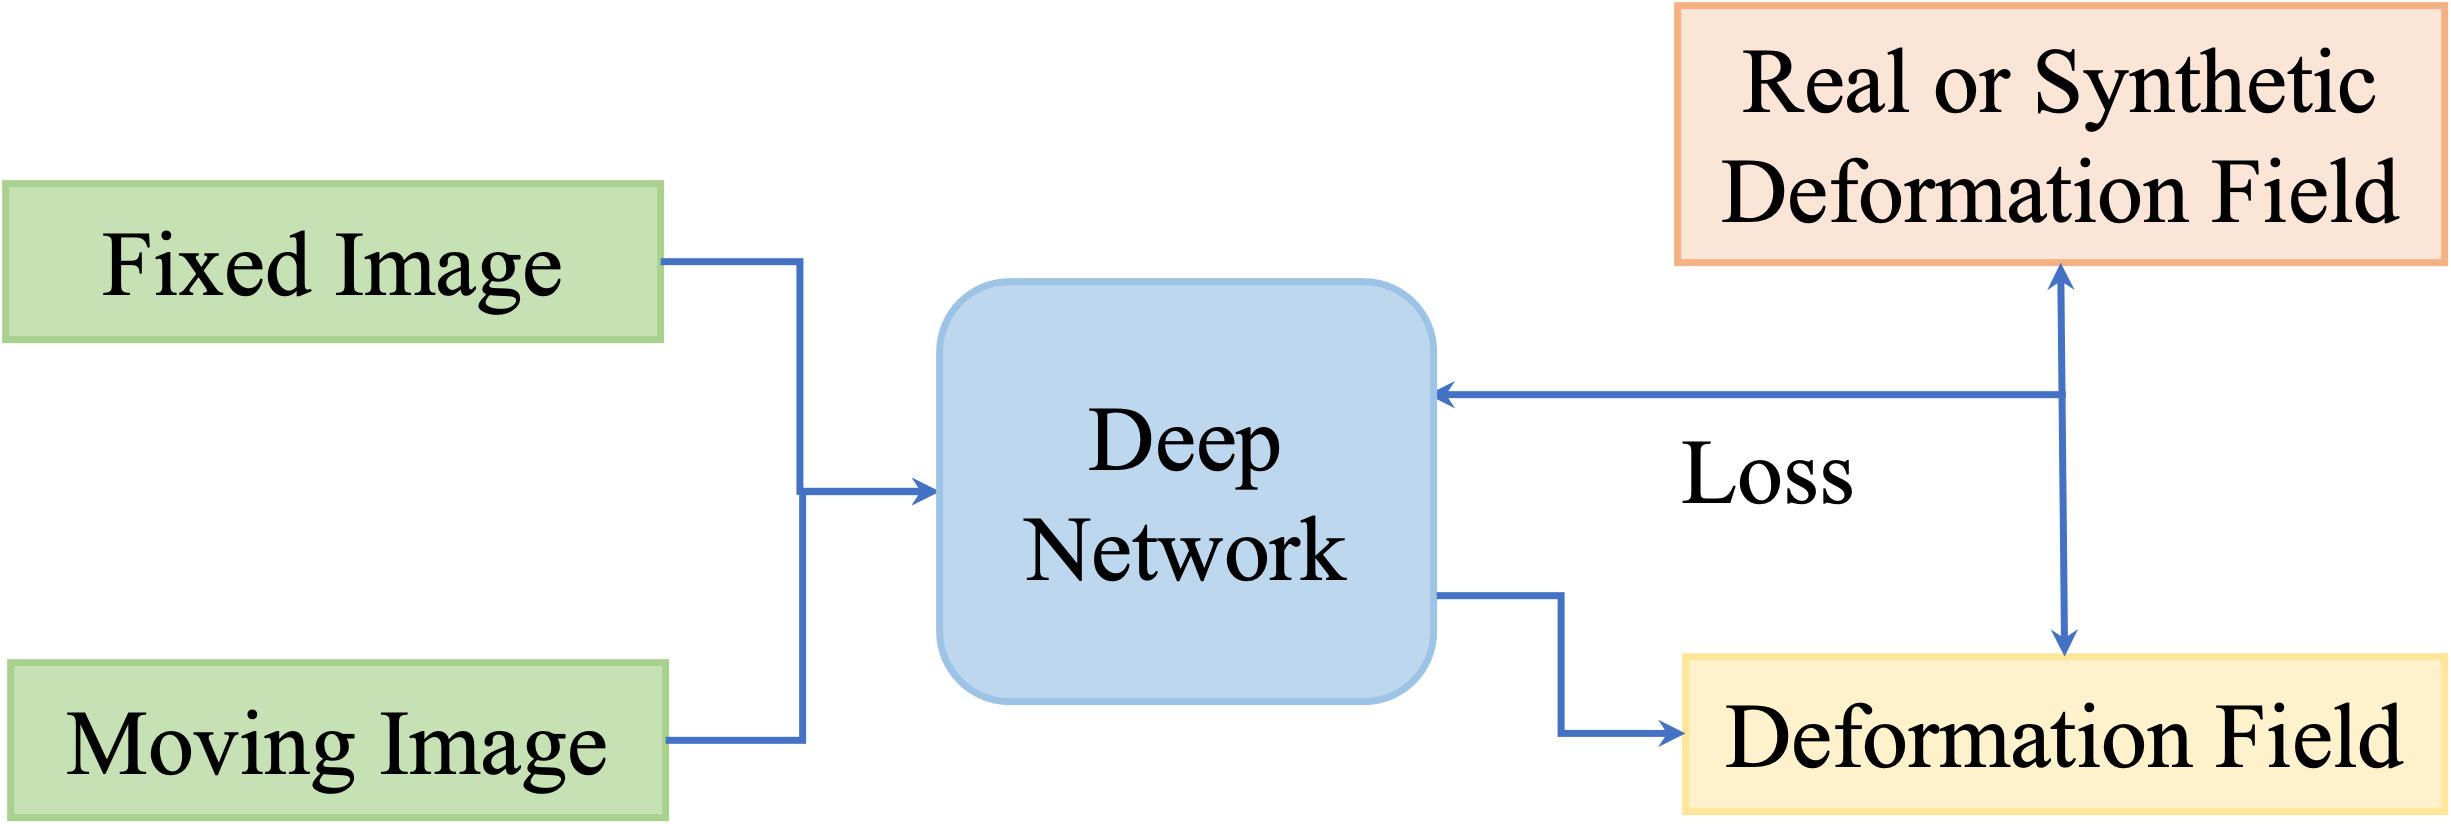
\includegraphics[width=\linewidth]{SupervisedRegistrationGraph.jpg} 
	\caption{Example graph illustrating the training process of a supervised network, taken from~\cite{Zou2022}.}
	\label{fig:SupervisedRegistration}
\end{figure}


\subsection{Unsupervised Registration} \label{SubSec:UnsupervisedRegistration}
As the preparation of the ground truth displacement field for supervised methods is inconvenient, limitations in generalizing results in different domains and various registration tasks are inevitable. Thus, unsupervised registration has a more convenient training process with paired images as inputs, but without a ground truth. Generally, unsupervised learning consists of similarity-based (see Figure~\ref{fig:UnsupervisedRegistration}) and GAN-based methods (see Figure~\ref{fig:GANRegistration}), where the loss function computes the similarity between the aligned images and the smoothness of the displacement field, rather than the difference to a ground truth~\cite{Zou2022}. Well known example are \emph{IC-Net}~\cite{IC-Net},  \emph{VoxelMorph}~\cite{Voxelmorph}, \emph{TransMorph}~\cite{TransMorph} and \emph{SYMNet}~\cite{SYM-Net}.

\begin{figure}[h] %tpb
	\centering
	\graphicspath{{images/}{\main/images/}}
	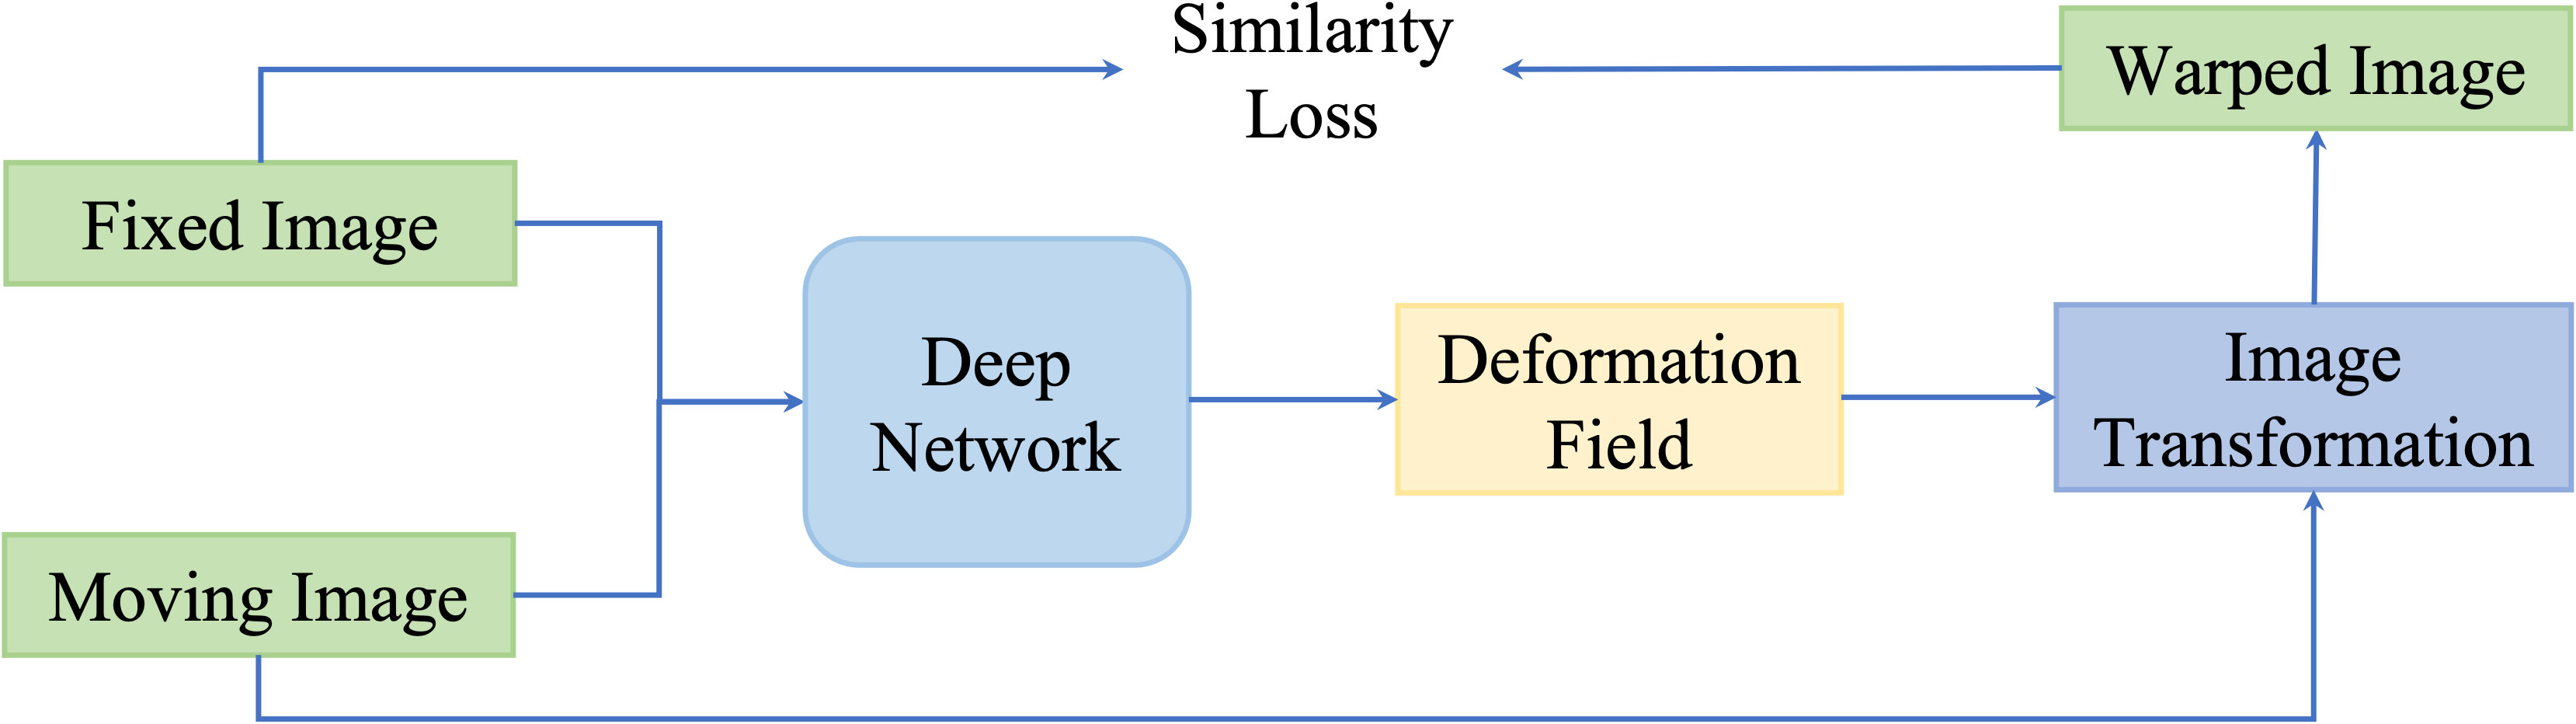
\includegraphics[width=\linewidth]{UnsupervisedRegistrationGraph.jpg} 
	\caption{Example graph illustrating the training process of an unsupervised network with only a image similarity loss, taken from~\cite{Zou2022}.}
	\label{fig:UnsupervisedRegistration}
\end{figure}

\begin{figure}[h] %tpb
	\centering
	\graphicspath{{images/}{\main/images/}}
	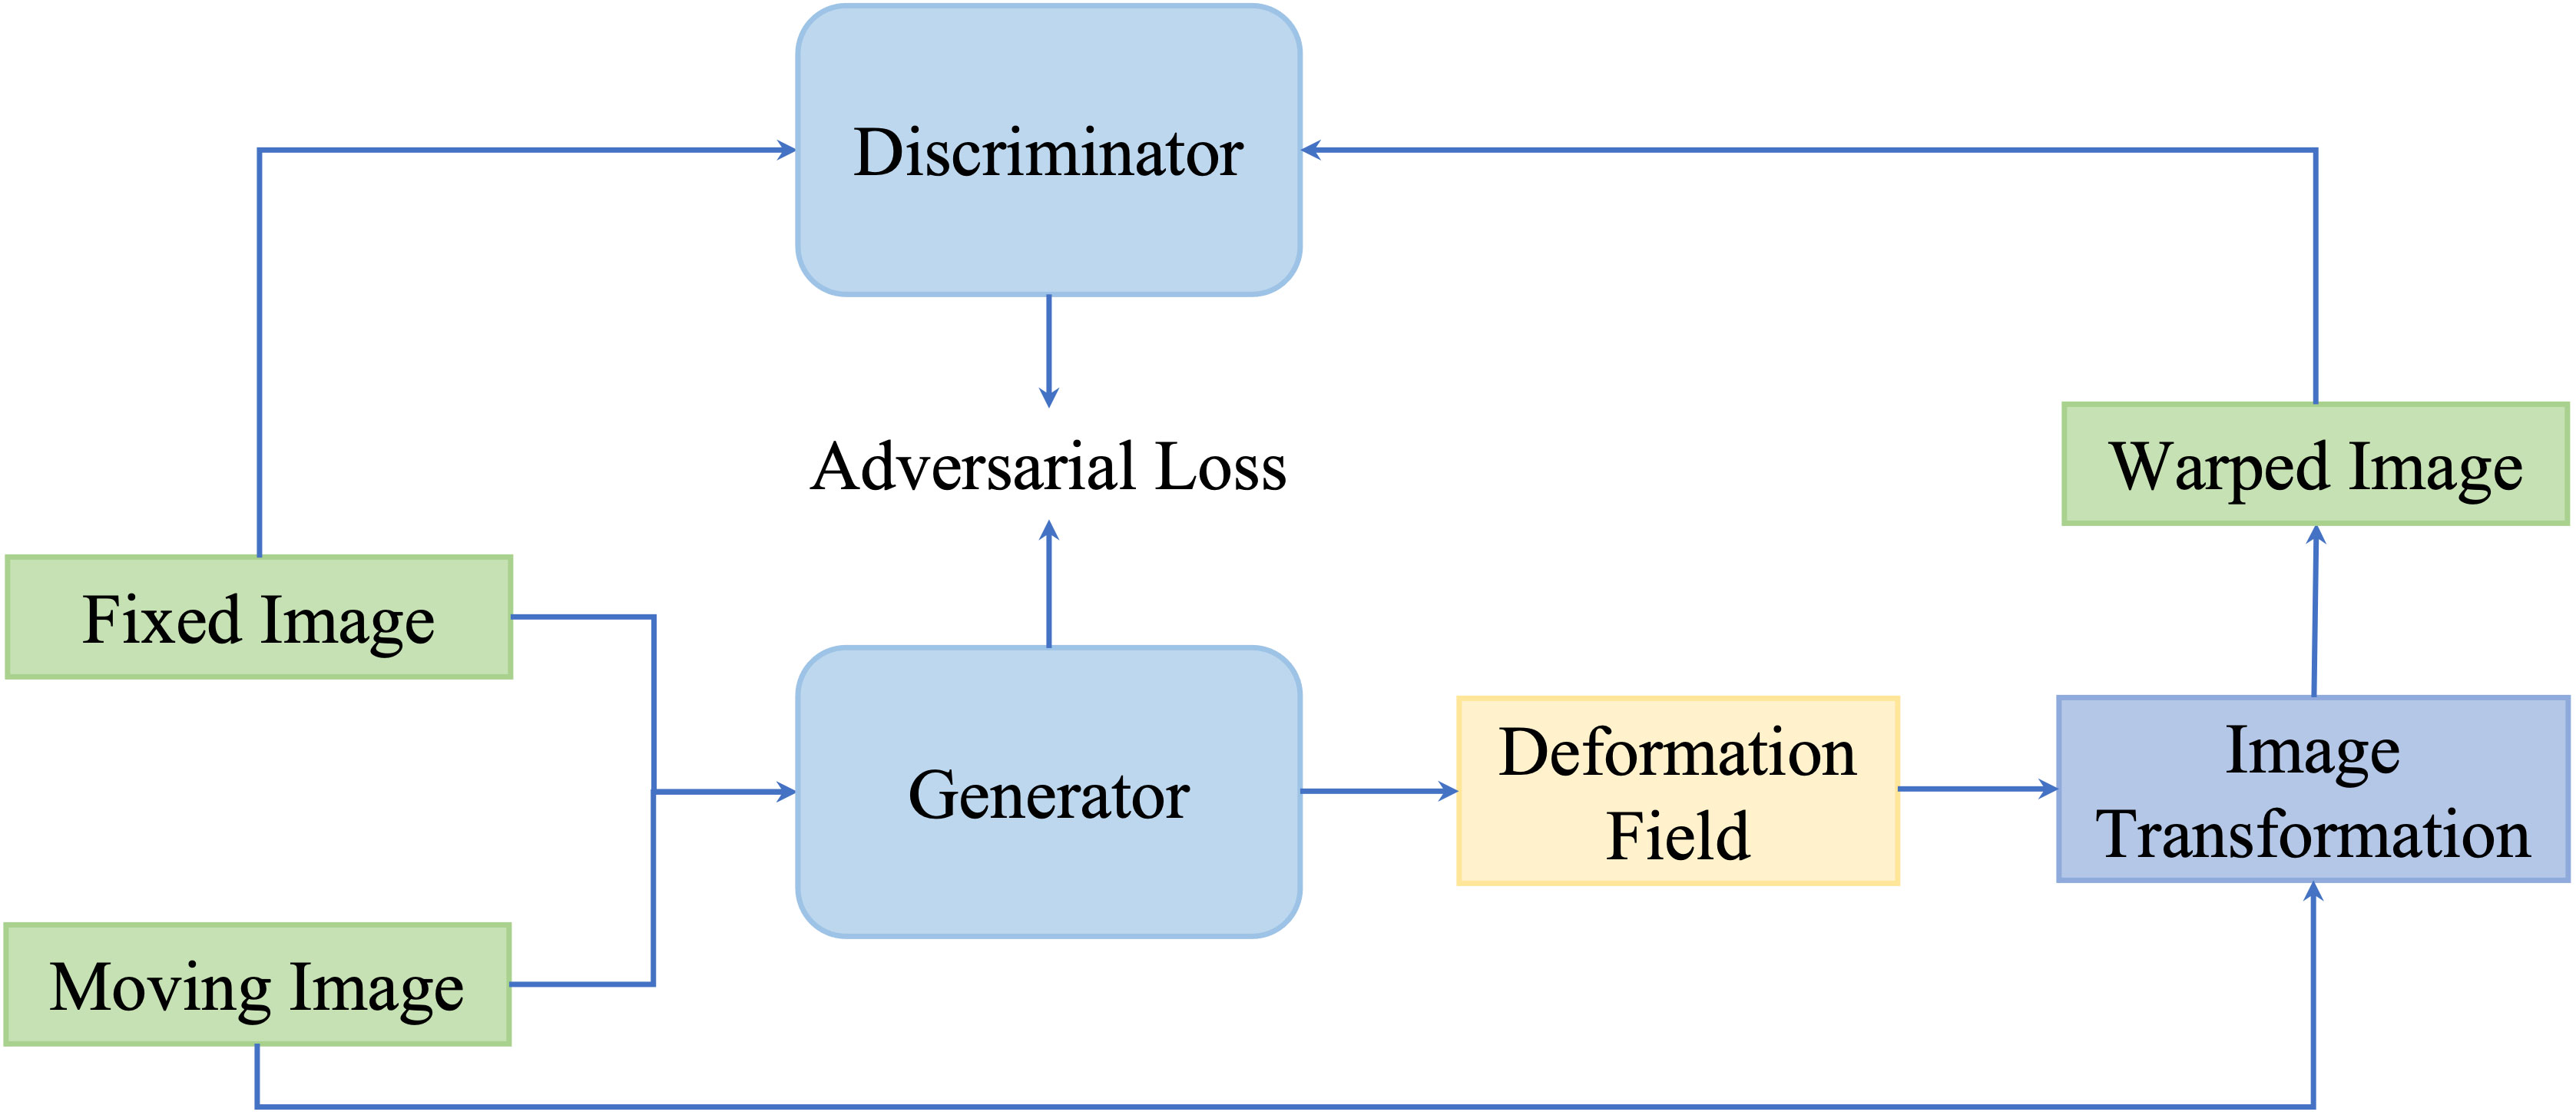
\includegraphics[width=\linewidth]{GANRegistrationGraph.jpg} 
	\caption{Example graph illustrating the training process of a GAN, taken from~\cite{Zou2022}.}
	\label{fig:GANRegistration}
\end{figure}

\subsection{Evaluation Metrics} \label{SubSec:EvalutionMetrics}
Different metrics can be used for evaluation of registration performance including similarity metrics and other stuff. The mean squared error (MSE) is calculated between a fixed (ground truth) image and the warped image giving a pixel-wise comparison:
\begin{equation}
	\text{MSE} = \frac{1}{N} \sum_{i=1}^{N} |F(x,y) - W(x,y)|^2,
\end{equation}
where $F$ is the fixed image and $W$ is the warped image with $N$ being the number of pixels in the images. The lower the MSE the higher the similarity with 0 being a perfect match (the images are exactly the same).\\

%Another common image metric is the normalized cross-correlation (NCC). 
%\begin{equation}
%	\text{NCC} = \frac{1}{N} \sum_{i=1}^{N} \frac{1}{\sigma_F \cdot \sigma_W} F(x,y) \cdot W(x,y),
%\end{equation}
%with image $F$ and $W$ as well as $N$ being the number of pixels in the images. \\

Another common image metric is the structural similarity index measure (SSIM), which operates between 1 (complete similarity) and 0 (no similarity) and tries to estimate the general similarity instead of a pixel-wise comparison making it more robust against contrast changes compared to e.g. MSE.
\begin{equation}
	\text{SSIM} = \frac{(2 \mu_F \mu_W + c_1) \cdot (2 \sigma_{FW} + c_2)}{(\mu_F^2 + \mu_W^2 + c_1) \cdot (\sigma_F^2 + \sigma_W^2 + c_2) },
\end{equation}
where $\mu_F, \mu_W$ are the mean values of the images $F$ and $W$; $\sigma_F^2, \sigma_W^2$ the variances of $F$ and $W$ as well as $\sigma_{FW}$ the covariance for $F$ and $W$, with $c_1, c_2$ being constants derived from the dynamic range of the images. \\
All of these metrics can also be used as loss functions for network training.\\
For comparison of segmentations the Dice score is a commonly used metric to estimate the similarity of two segmentations. A score of 1 indicates a complete overlap/match and a score of 0 indicates no overlapping of the segmentations. The Dice score is calculated as follows:
\begin{equation}
	\text{Dice} = \frac{2 |M_F \cap M_W|}{|M_F| + |M_W|},
\end{equation}
with $M_F$ and $M_W$ being segmentations corresponding to $F$ and $W$ with $M_F$ being a manual segmentation which is warped to obtain $M_W$~\cite{NiftiReg}.\\
Aside from image similarity measures and the evaluation of image segmentations, the displacement field itself can also be evaluated. This is usually based on the assumption that the displacement should be smooth as, for example, folding the image could result in physically unrealistic anatomic structures, indicating errors. The Jacobian determinant of the deformation $|J_{\phi}|$ must be positive everywhere to avoid folding and thus the percentage of non-positive Jacobian determinant of the deformation $\% \, |J_{\phi}|\leq0$ can be used to evaluate the quality of the generated displacement field~\cite{Chen2023}.


%%%%%%%%%%%%%%%%%%%%%%%%
%%%%%  Methodology %%%%%
%%%%%%%%%%%%%%%%%%%%%%%%

%\chapter{Methodology}
%In this chapter the main part of the actual work is discussed.

\chapter{Data}	\label{Ch:Data}
In the following chapter, the datasets used in this thesis are presented and potential pre-processing steps, as well as uses, discussed. The first dataset called \emph{OASIS}, containing MRI brain scans, was used in the original publications for training and evaluation of both \emph{Fourier-Net} and \emph{Fourier-Net+}. It was thus used to get familiar with these networks and their respective work-flows as well as reproducing some results from the paper to ensure that the code works as intended.\\ 
For our major experiment the \emph{CMRxRecon} dataset was used. The cardiac MRI k-space data was used for extending the networks to frame-to-frame registration in order for them to be integrated into a motion reconstruction pipeline. It already contains subsampled data, but does not provide segmentations for multi-coil data.\\
Thus a third dataset, the \emph{ACDC} cardiac dataset, was used. While it contains no k-space data segmentations are given for end-systolic and end-diastolic frames, which can thus be used for the evaluation of registration performance. Most parameter studies and optimizations of the networks were done with this dataset.

\section{OASIS Dataset} \label{Sec:OASIS}
The \emph{OASIS-1} dataset~\cite{OASIS} contains T1-weighted MRI brain scans from 454 subjects and was mainly used for training and testing the original \emph{Fourier-Net/Fourier-Net+}. The brain scans were further pre-processed by~\cite{HyperMorph} for the \emph{Learn2Reg}-Challenge~\cite{Learn2Reg}. This enables subject-to-subject brain registration, as all MRI scans were bias-corrected, skull-stripped, aligned, and cropped to the size of $160 \times 192 \times 224$. The images were stored in the \emph{NIFTI} format,  which makes it really easy to use. Examples can be seen in Figures~\ref{fig:image1} and \ref{fig:image2} with slices from the center of the x-, y- and z-axis.

\begin{figure}[h]%tpb
	\centering
	\graphicspath{{images/}{\main/images/}}
	\begin{subfigure}{0.45\textwidth}
    		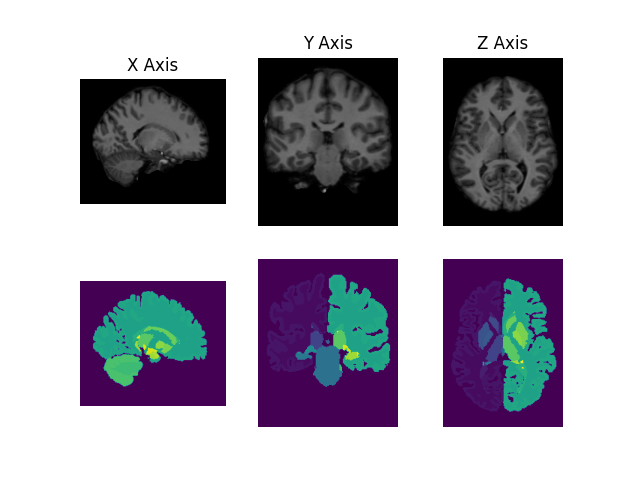
\includegraphics[width=\textwidth]{image2.png}
    		%\caption{Example Image from the Dataset with corresponding labels.}
		\caption{}    		
    		\label{fig:image2}
	\end{subfigure}
	\hfill
	\begin{subfigure}{0.45\textwidth}
    		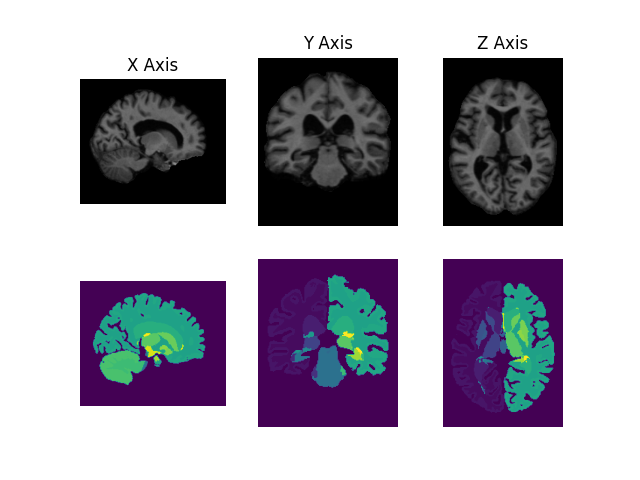
\includegraphics[width=\textwidth]{image1.png}
    		%\caption{Another example Image from the Dataset with corresponding labels.}
		\caption{}    		
    		\label{fig:image1}
	\end{subfigure}
	\caption{Example images (upper row) from the \emph{OASIS} dataset with corresponding labels (bottom row).}
	\label{fig:OASIS}
\end{figure}

\section{CMRxRecon Dataset} \label{Sec:CMRxRecon}
The \emph{CMRxRecon} dataset~\cite{CMRxRecon} from the \emph{CMRxRecon2023} challenge specializes in Cardiac magnetic resonance imaging (CMR). The dataset includes 
%multi-contrast k-space data, consisting of cardiac cine, T1/T2-mapping, tagging, phase-contrast (i.e., flow2d), and dark-blood imaging
fully sampled and subsampled multi-coil k-space data, as well as auto-calibration lines. This includes imaging of different anatomical views like long-axis (2-chamber, 3-chamber, and 4-chamber) and short-axis (SAX). There is a total of 120 training data, 60 validation data, and 120 test data from healthy volunteers. One of the goals of the challenge is the reconstruction from subsampling and motion correction for the heart movement.

\subsection{Image Reconstruction} \label{SubSec:ImageReconstruction}
As the data was recorded in the k-space (see Figure~\ref{fig:k-space}) and stored as \emph{.mat} files we first need to reconstruct the images to use them for training and testing of \emph{Fourier-Net/Fourier-Net+}. For this, multi-coil reconstruction algorithms like \emph{SENSE}~\cite{SENSE1} can be used. The sensitivity of the different coils can be seen in Figure~\ref{fig:Coils}, where each coil focuses on a specific area of the image. These images are then stitched together in reconstruction to produce a combined image with great overall contrast.
%, while Figure~\ref{fig:ImageSlice} contains the complete reconstructed image. 
The dataset, as mentioned before, contains fully sampled as well as subsampled k-space data (see Figure~\ref{fig:fullySampled} and Figure~\ref{fig:subSampled}), with the latter being typically used to accelerate the MRI acquisition process. This is done by not using all of the available k-space data, but rather masking the signal to achieve the subsampling. The center region of the k-space is always fully sampled, but the outer regions are subsampled depending on the sampling strategy~\cite{SamplingStrategies}. The dataset contains subsampled k-space data for 4x and 8x acceleration with the latter of course leading to more distortions in the reconstructed image as the subsampling can induce image reconstruction artifacts. This can be seen in Figure~\ref{fig:subSampledImage}, where the image reconstructed from 4x accelerated k-space data seems blurred when compared to the fully sampled one in Figure~\ref{fig:fullySampledImage}. 
%An example image can be seen in Figure~\ref{fig:Subsampling} where the k-space of the original image is subsampled with a random mask leading to heavy blurring artifacts after the reconstruction.
For all experiments the short-axis  view data was used. As image sizes between patients can vary slightly, interpolation was used to standardize the images to a size of $246 \times 512$ to avoid further problems with e.g. 
%ensure coherent sizes between images to avoid problems with the network and 
loss calculation. Additionally, min-max-normalization is used to standardize the data range for all images to $[0,1]$ as this was also varying. The reconstructed images were stored for every image slice for every patient. Thus, all frames for a specific image slice were in a single folder to enable easy access for later data load-in for frame-to-frame registration.

\begin{figure}[h]%tpb
	\centering
	\graphicspath{{images/}{\main/images/}}
	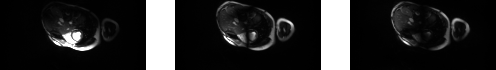
\includegraphics[width=\linewidth]{CoilsHorizontal.png} 
	\caption{MRI images for three different coils from the \emph{CMRxRecon} dataset~\cite{CMRxRecon}.}
	\label{fig:Coils}
\end{figure}


\begin{figure}[h]%tpb
	\centering
	\graphicspath{{images/}{\main/images/}}
	\begin{subfigure}{0.45\textwidth}
    		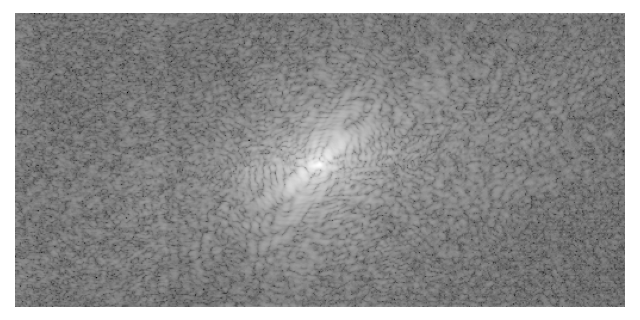
\includegraphics[width=\textwidth]{k-space_fullysampled.png}
    		\caption{Example for a fully sampled k-space with the low frequencies in the middle.}
    		\label{fig:fullySampled}
	\end{subfigure}
	\hfill
	\begin{subfigure}{0.45\textwidth}
    		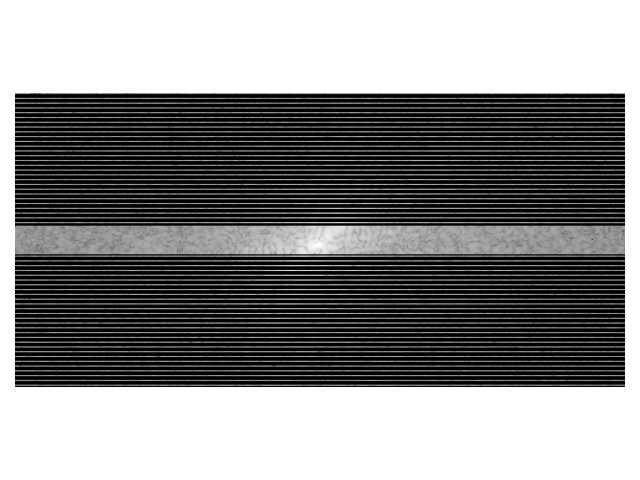
\includegraphics[width=\textwidth]{k-space_subsampled.png}
    		\caption{Example of a subsampled k-space for 4x acceleration.}
    		\label{fig:subSampled}
	\end{subfigure}\\
	\begin{subfigure}{0.45\textwidth}
    		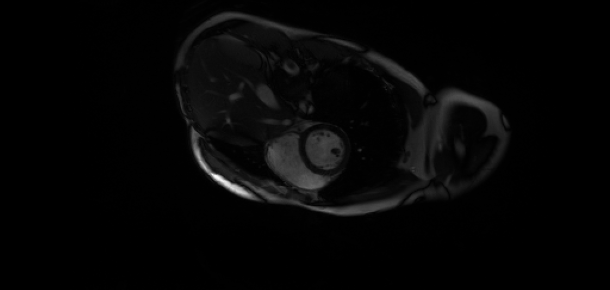
\includegraphics[width=\textwidth]{image_fullysampled.png}
    		\caption{Corresponding image reconstructed from the fully sampled k-space.}
    		\label{fig:fullySampledImage}
	\end{subfigure}
	\hfill
	\begin{subfigure}{0.45\textwidth}
    		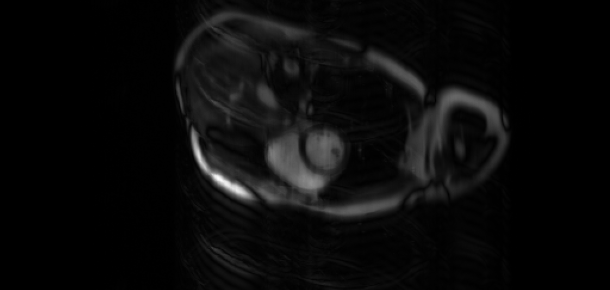
\includegraphics[width=\textwidth]{image_subsampled.png}
    		\caption{Corresponding image reconstructed from the subsampled k-space.}
    		\label{fig:subSampledImage}
	\end{subfigure}
	\caption{Fully sampled and subsampled k-space data from the from the \emph{CMRxRecon} dataset~\cite{CMRxRecon} with corresponding images.}
	\label{fig:k-space}
\end{figure}


%\begin{figure}[htpb]
%	\centering
%	\graphicspath{{images/}{\main/images/}}
%	\begin{subfigure}{0.4\textwidth}
%    		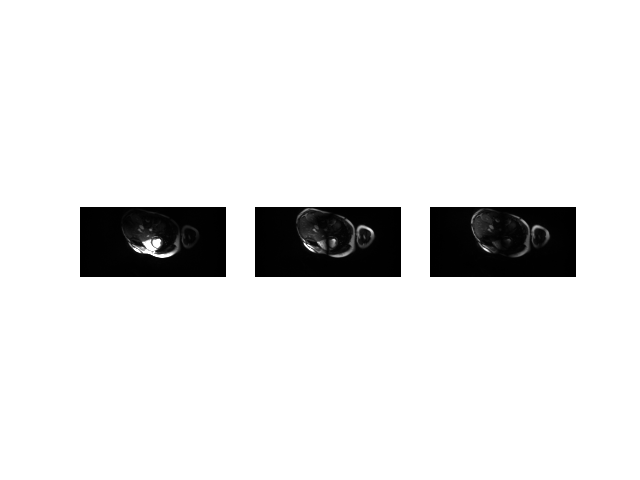
\includegraphics[width=.75\textwidth]{Coils.png}
%    		\caption{MRI images for three different coils.}
%    		\label{fig:Coils}
%	\end{subfigure}
%	\hfill
%	\begin{subfigure}{0.4\textwidth}
%    		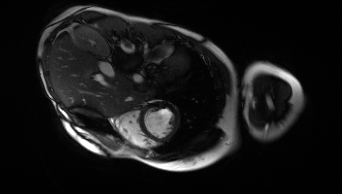
\includegraphics[width=\textwidth]{ImageSlice.png}
%    		\caption{Reconstructed image from the three different coils.}
%    		\label{fig:ImageSlice}
%	\end{subfigure}
%	\caption{Example from the \emph{CMRxRecon} dataset.}
%	\label{fig:CMRxRecon}
%\end{figure}

%\begin{figure}[htpb]
%	\centering
%	\graphicspath{{images/}{\main/images/}}
%	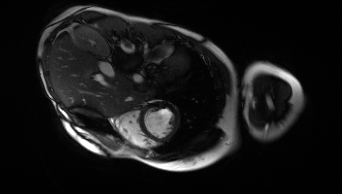
\includegraphics[width=.5\linewidth]{ImageSlice.png} 
%	\caption{Reconstructed image slice from the different coils from the \emph{CMRxRecon} dataset~\cite{CMRxRecon}.}
%	\label{fig:ImageSlice}
%\end{figure}

%\begin{figure}[htpb]
%	\centering
%	\graphicspath{{images/}{\main/images/}}
%	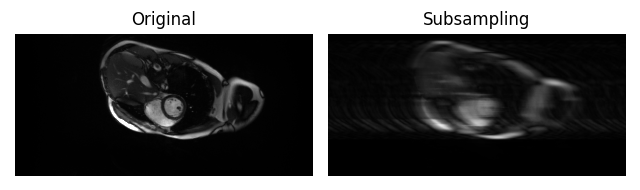
\includegraphics[width=\linewidth]{Subsampling.png} 
%	\caption{Example for blurring artifacts encountered during image reconstruction after subsampling the k-space.}
%	\label{fig:Subsampling}
%\end{figure}

\subsection{Pre-Processing} \label{SubSec:Pre-Processing}
As seen before, a large part of the image is just black background that contains no usable information. The interesting cardiac region in the image, however, is much smaller and thus image cropping can be used to extract it. The fairly large image size can thus be cut down without losing important image information, which also helps with memory efficiency. One problem however remains: image alignment. Whereas in the \emph{OASIS} dataset the brain scan were already aligned, the cardiac data in the \emph{CMRxRecon} dataset is not. Thus, one cannot simply center-crop all images as the cardiac region might be located in very different parts of the image. To resolve this issue, adaptive cropping with automatic detection of the cardiac region in the images is needed. \\
To begin, some assumption about the data needs to be made: First, the cardiac region is at the same position for all slices and frames from one patient. Second, most of the movement happens in the cardiac region between frames. From the latter we can conclude that we need to examine the frames, thus the difference between consecutive frames is calculated and averaged for each slice. According to the first assumption this process is repeated for all slices and their results summed to create a sort of heatmap as seen in Figure~\ref{fig:SumDifferences} with a clearly higher intensity in the cardiac region compared to the background. To further isolate this region a simple thresholding is performed followed by an opening operation, which removes any smaller fragments still left in the image. The cardiac region is now clearly separated from the rest of the image as seen in Figure~\ref{fig:MaskCropping}. The only step left is to calculate the approximate center of this region and create a crop around it. To drastically reduce the image size a cropping factor of one third was used, reducing the image size from $246 \times 512$ to $82 \times 170$. The result of this drastic crop can be seen in Figure~\ref{fig:ImageCropped} when compared to the original image in Figure~\ref{fig:fullImage}. Note, however, that the cropped image in Figure~\ref{fig:ImageCropping} appears larger than it actually is, when compared to the original, to allow for a more detailed look. Thus both images are not presented to scale, but in order to show the most image detail.

\begin{figure}[h]%tpb
	\centering
	\graphicspath{{images/}{\main/images/}}
	\begin{subfigure}{0.4\textwidth}
    		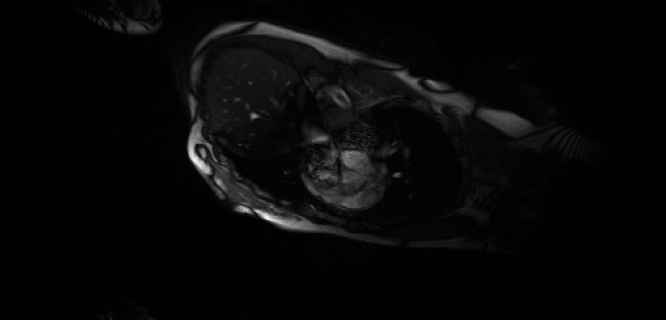
\includegraphics[width=\textwidth]{FullImage.png}
    		\caption{The original full-size image.}
    		\label{fig:fullImage}
	\end{subfigure}
	\hfill
	\begin{subfigure}{0.4\textwidth}
    		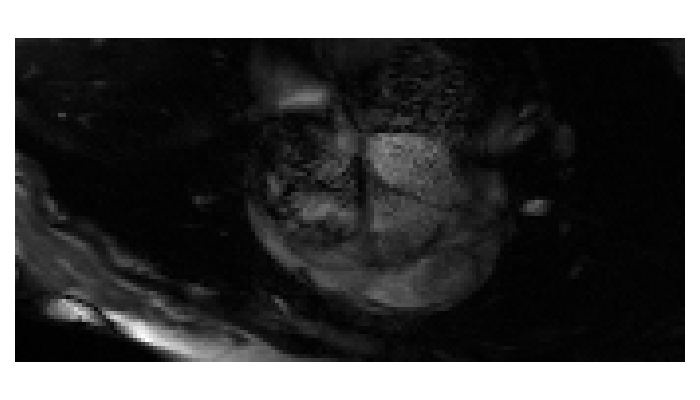
\includegraphics[width=\textwidth]{ImageCrop.png}
    		\caption{The corresponding cropped image.}
    		\label{fig:ImageCropped}
	\end{subfigure}
	\\
	\begin{subfigure}{0.4\textwidth}
    		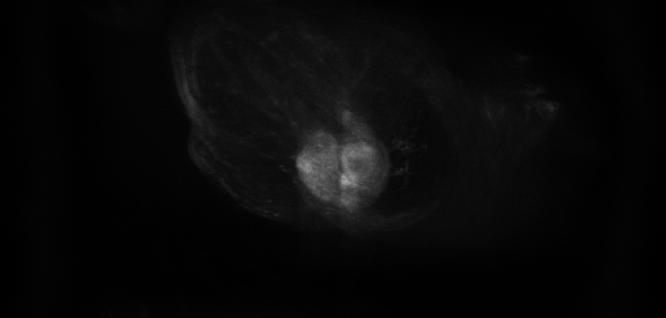
\includegraphics[width=\textwidth]{DifferencesSlices.png}
    		\caption{Sum of the differences between slices and their respective frames with the cardiac region in the middle.}
    		\label{fig:SumDifferences}
	\end{subfigure}
	\hfill
	\begin{subfigure}{0.4\textwidth}
    		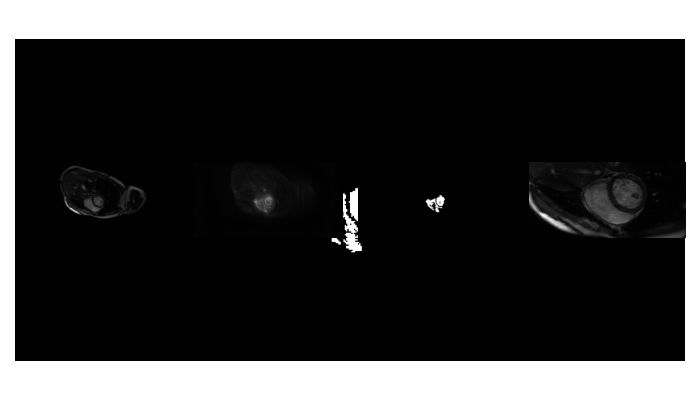
\includegraphics[width=\textwidth]{MaskForCropping.png}
    		\caption{Mask of the cardiac region generated from the sum of differences by thresholding and opening.}
    		\label{fig:MaskCropping}
	\end{subfigure}
	\caption{Cropping of an example image by locating the movement between frames for each slice. Note that the cropped image appears larger than it actually is compared to the original.}
	\label{fig:ImageCropping}
\end{figure}

%\begin{figure}[htpb]
%	\centering
%	\graphicspath{{images/}{\main/images/}}
%	\begin{subfigure}{0.6\textwidth}
%    		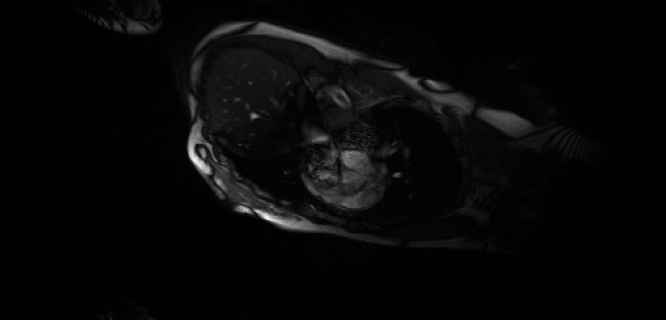
\includegraphics[width=\textwidth]{FullImage.png}
%    		\caption{The original full-size image.}
%    		\label{fig:fullImage}
%	\end{subfigure}
%	\\
%	\begin{subfigure}{0.6\textwidth}
%    		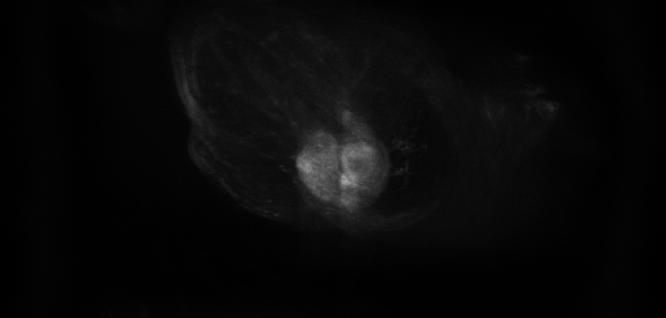
\includegraphics[width=\textwidth]{DifferencesSlices.png}
%    		\caption{Sum of the differences between slices and their respective frames with the cardiac region in the middle.}
%    		\label{fig:SumDifferences}
%	\end{subfigure}
%	\\
%	\begin{subfigure}{0.6\textwidth}
%    		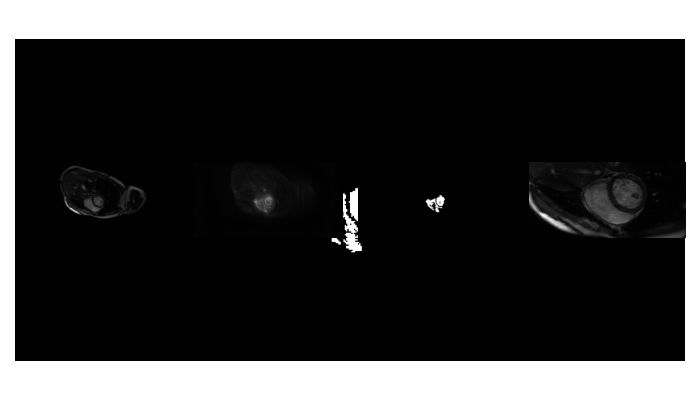
\includegraphics[width=\textwidth]{MaskForCropping.png}
%    		\caption{Mask of the cardiac region generated from the sum of differences by thresholding and opening.}
%    		\label{fig:MaskCropping}
%	\end{subfigure}
%	\\
%	\begin{subfigure}{0.6\textwidth}
%    		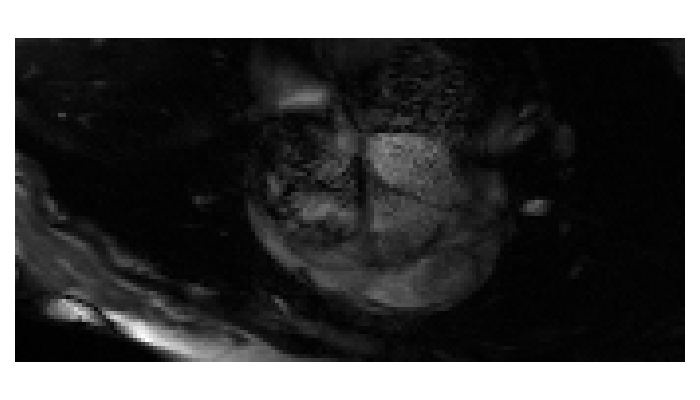
\includegraphics[width=\textwidth]{ImageCrop.png}
%    		\caption{The corresponding cropped image.}
%    		\label{fig:ImageCropped}
%	\end{subfigure}
%	\caption{Cropping of an example image by locating the movement between frames for each slice. Note that the cropped image appears larger than it actually is compared to the original.}
%	\label{fig:ImageCropping}
%\end{figure}

\section{ACDC Dataset}
The \emph{ACDC} dataset~\cite{ACDC} from the \emph{Automated Cardiac Diagnosis Challenge (ACDC)} during the \emph{MICCAI 2017} conference. It contains cardiac cine-MRI short-axis data from 150 subjects that were divided into 5 subgroups (4 pathological, 1 healthy). For each subject systolic (see Figure~\ref{fig:Image_ACDC_systolic}) and diastolic frames (see Figure~\ref{fig:Image_ACDC_diastolic}) are provided with corresponding segmentations (see Figure~\ref{fig:Segmentation_ACDC_systolic} and ~\ref{fig:Segmentation_ACDC_diastolic}), which enables direct comparison via e.g. the Dice score. The segmentations contain only four values with 0, 1, 2 and 3 representing pixels located in the background, in the RV cavity, in the myocardium, and in the LV cavity. The frames themselves are 3D volumes with size $216 \times 256 \times 10$, thus ten image slices can be extracted which each have size $216 \times 256$. The same holds true for the segmentation, which means that both the image data and segmentations can generated in the same manner.\\
For the training data, the original 4D data was used as we do not require the segmentations for the end-systolic and end-diastolic frames. As the 4D data has size $216 \times 256 \times 10 \times 30$ we can extract 30 frames for each of the ten slices. These can be sorted into 251376 image pairs for training. For the validation and test data the end-systolic and end-diastolic frames with their segmentations were used given us 641 image pairs each as we can only have these two frames to align.

\begin{figure}[h]%tpb
	\centering
	\graphicspath{{images/}{\main/images/}}
	\begin{subfigure}{0.4\textwidth}
    		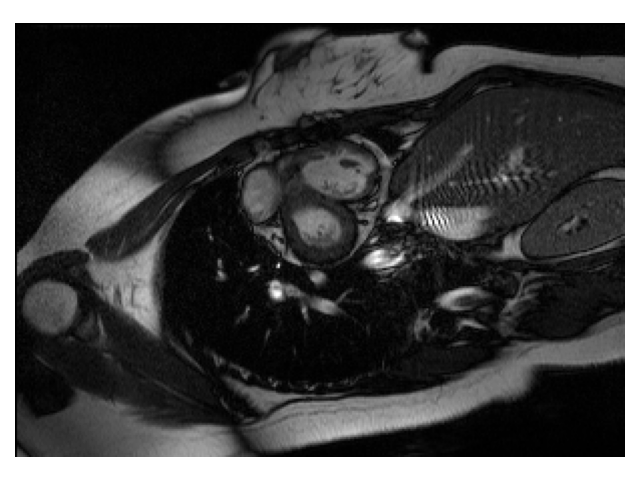
\includegraphics[width=\textwidth]{Image_ACDC_systolic.png}
    		\caption{Image of systolic phase.}
    		\label{fig:Image_ACDC_systolic}
	\end{subfigure}
	\hfill
	\graphicspath{{images/}{\main/images/}}
	\begin{subfigure}{0.4\textwidth}
    		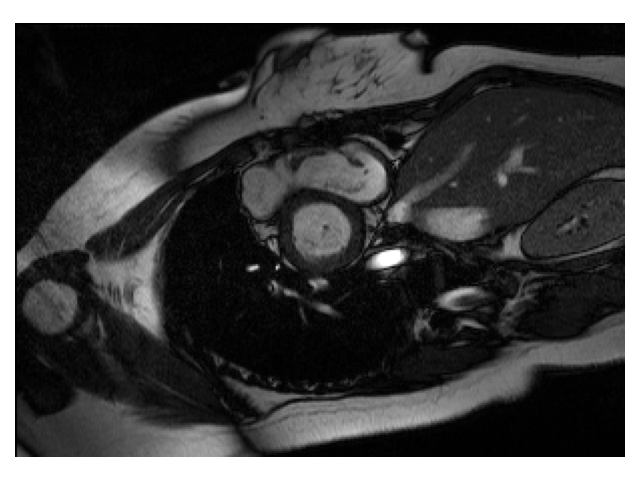
\includegraphics[width=\textwidth]{Image_ACDC_diastolic.png}
    		\caption{Image of diastolic phase.}
    		\label{fig:Image_ACDC_diastolic}
	\end{subfigure} 
	\\
	\begin{subfigure}{0.4\textwidth}
    		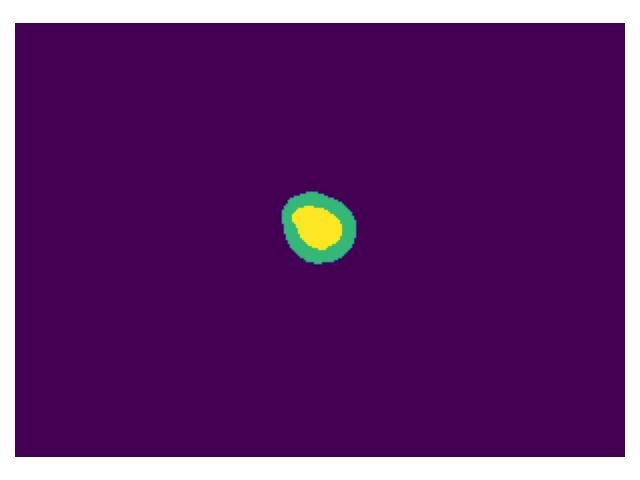
\includegraphics[width=\textwidth]{Segmentation_ACDC_systolic.png}
    		\caption{Segmentation of systolic phase.}
    		\label{fig:Segmentation_ACDC_systolic}
	\end{subfigure}
	\hfill
	\begin{subfigure}{0.4\textwidth}
    		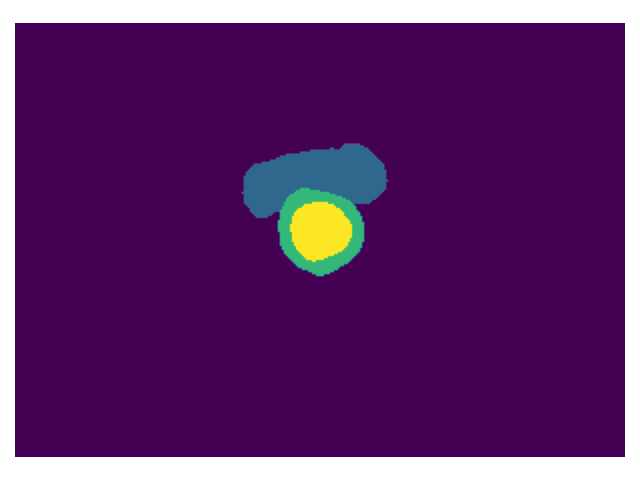
\includegraphics[width=\textwidth]{Segmentation_ACDC_diastolic.png}
    		\caption{Segmentation of diastolic phase.}
    		\label{fig:Segmentation_ACDC_diastolic}
	\end{subfigure}
	\caption{Example images for systolic (a) and diastolic frames (b) with corresponding segmentations (c),(d) taken from the \emph{ACDC} dataset~\cite{ACDC}.}
	\label{fig:}
\end{figure}


\chapter{Network Architectures} \label{Ch:NetworkArchitecture}
As a starting point \emph{Fourier-Net}~\cite{Fourier-Net} and its successor \emph{Fourier-Net+}~\cite{Fourier-Net+} were used. These networks, which are explained in the following pages, enable fast and accurate registration while needing less resources compared to similar approaches. These attributes are very beneficial for a potential application like motion correction because the current networks, e.g. \emph{LAPNet}~\cite{LAPNet}, are usually supervised and require large computational resources.

\section{Fourier-Net}	\label{Sec:Fourier-Net}
\emph{Fourier-Net} is a new unsupervised approach that aims to learn a low-dimensional representation of the displacement field in a band-limited Fourier domain instead of the full field in the spatial domain. This band-limited representation is then decoded by a model-driven decoder to the dense, full-resolution displacement field in the spatial domain. This allows for fewer parameters and computational operations, resulting in faster inference speeds~\cite{Fourier-Net}. The architecture is based on the U-Net~\cite{U-Net}, like most deep registration approaches, but replaces the expanding path with a parameter-free model-driven decoder as mentioned before. The encoder of \emph{Fourier-Net} consists of a CNN, which takes two images (fixed and moving) as inputs. The output is a displacement field that is then converted from the spatial domain into the Fourier domain via an discrete Fourier transformation (DFT). From there, this band-limiting representation 
%of the displacement field 
is padded with zeros to the full resolution of the original displacement field. The field is then recovered by using the inverse DFT (iDFT) to convert it back into the spatial domain. This displacement field is then used to warp the moving image into the fixed image. Additionally, squaring and scaling layers~\cite{Dalca2018} can be added before warping the image in order to encourage a diffeomorphism in final deformation. 

\begin{figure}[htpb]
	\centering
	\graphicspath{{images/}{\main/images/}}
	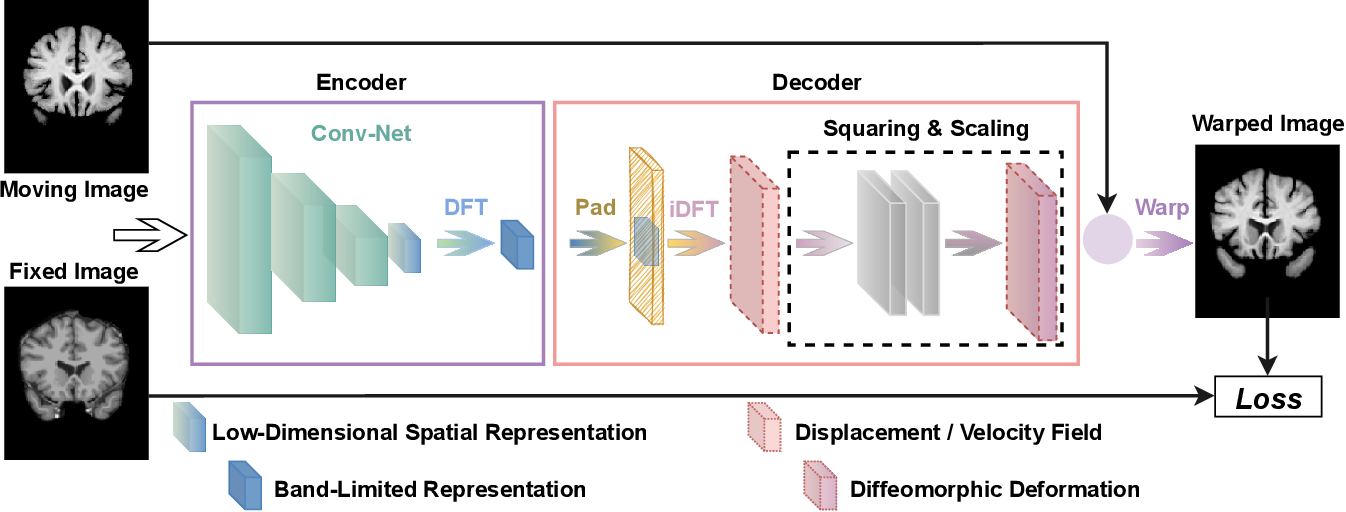
\includegraphics[width=\linewidth]{ArchitectureFourier-Net.png} 
	\caption{Architecture of \emph{Fourier-Net} taken from~\cite{Fourier-Net}.}
	\label{fig:Fourier-Net}
\end{figure}

\subsection{Encoder}	\label{SubSec:Encoder}
The encoder of \emph{Fourier-Net} consists of a CNN that generates the displacement field between the two inputs followed by a DFT layer that produces a band-limited representation of the full displacement field. The fully convolutional neural network (FCN) from \emph{SYMNet}~\cite{SYM-Net} was modified to function as the CNN of the encoder. Its (original) architecture (see Figure~\ref{fig:SYMNet}) is again based on the \emph{U-Net} with a contracting and expanding path. 
\begin{figure}[htpb]
	\centering
	\graphicspath{{images/}{\main/images/}}
	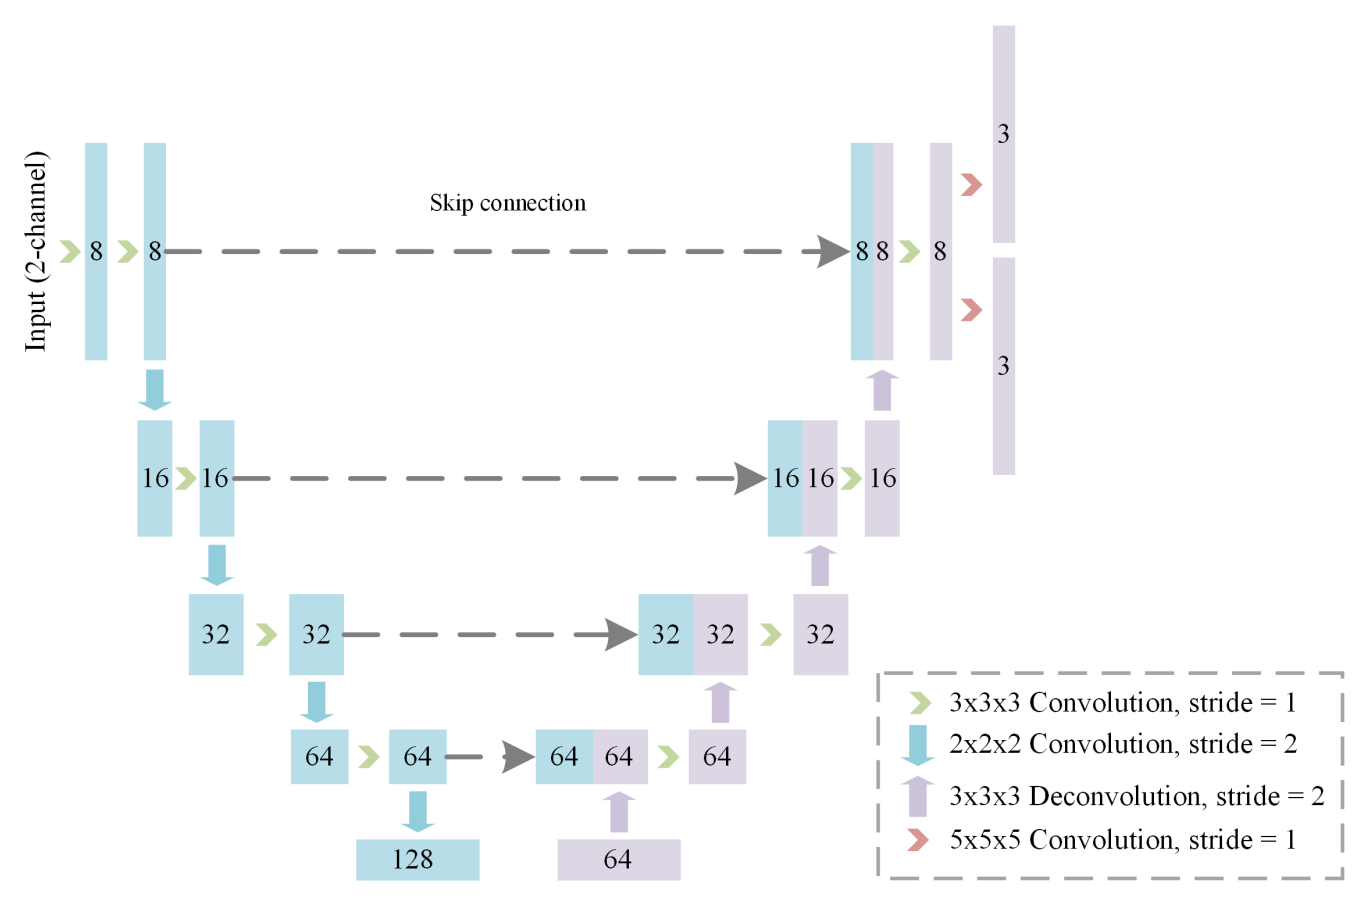
\includegraphics[width=\linewidth]{SYMNetArchitectureFCN.png} 
	\caption{Architecture of the FCN from \emph{SYMNet}~\cite{SYM-Net}.}
	\label{fig:SYMNet}
\end{figure}
The FCN concatenates the inputs images $X$ and $Y$ as a single 2-channel input and estimates two dense, non-linear displacement fields $\phi_{XY}$ and $\phi_{YX}$, however we only need the displacement field for the moving image, denoted as $\mathbb{S}_\phi$, since we are not interested in transforming the fixed image. This is actually a low dimensional representation because \emph{Fourier-Net} does not utilize the last two levels of the FCNs expanding path that would be needed to reconstruct the actual full-resolution displacement field $\phi$.\\
For each level in the contracting path of the FCN, two successive convolution layers are applied, which contain one $3 \times 3 \times 3$ convolution layer with a stride of 1, followed by a $3 \times 3 \times 3$ convolution layer with a stride of 2 to further compute the high-level features between the input images as well as downsample the features by half until the lowest level of the network is reached. For each level in the expanding path of the FCN, the feature maps from the contracting path are concatenated through skip connections and apply $3 \times 3 \times 3$ convolution with a stride of 1 and $2 \times 2 \times 2$ deconvolution layer for upsampling the feature maps to twice of its size. At the end of the expanding path, two $5 \times 5 \times 5$ convolution layers with a stride of 1 are appended to the last convolution layer and generate the displacement fields $\theta_{XY}$ and $\theta_{YX}$~\cite{SYM-Net}. Each convolution layer in the FCN is followed by a rectified linear unit (ReLU) activation, except for the output convolution layer that does not have an activation function because \emph{Fourier-Net} only uses the first two levels of the expanding path, thus leading the FCN to generate a low dimensional representation $\mathbb{S}_\phi$ of the full-resolution displacement field $\phi$.\\
%, where a SoftSign activation function is used~\cite{SYM-Net}:
%\begin{equation}
%	\text{SoftSign}(x) = \frac{x}{1 + |x|} .
%\end{equation}
As discussed previously, the encoder aims to learn a displacement (or velocity) field in the band-limited Fourier domain. Intuitively, this may require convolutions to be able to handle complex-valued numbers, which can be done by using complex-valued CNNs~\cite{Trabelsi2017}, which are suitable when both input and output are complex values, however these complex-valued operations sacrifice computational efficiency. Other approaches like \emph{DeepFlash}~\cite{DeepFlash} tackle this problem by converting the input images to the Fourier domain and using two individual real-valued CNNs to learn the real and imaginary parts separately. This, however, increases training and inference cost. To bridge the domain gap between real-valued spatial images and complex-valued band-limited displacement fields without increasing complexity, \emph{Fourier-Net} uses a DFT layer after the FCN. This is a simple and effective way to produce complex-valued band-limited displacement fields without the network needing to be able to handle complex values itself. The DFT applied to the displacement field $\phi$ can be defined as follows:
\begin{equation} \label{eq:DFT}
	[\mathcal{F}(\phi)]_{k,l} = \sum^{H-1}_{n=0} \sum^{W-1}_{m=0} \phi_{n,m} \cdot \exp \Bigg(i \cdot \bigg(\frac{2 \pi k}{H} \cdot n + \frac{2 \pi l}{W} \cdot m \bigg) \Big),
\end{equation}
where $\phi$ has size $H \times W$, $n \in [0,H-1]$ and $m \in [0,W-1]$ are the discrete indices in the spatial domain, and $k \in [0,H-1]$ and $l \in [0,W-1]$ are the discrete indices in the frequency domain with $i$ being the imaginary unit. However, $\phi$ in this equation is actually the low dimensional representation of the displacement field output by the modified FCN, which can be formulated as follows:
\begin{equation} \label{eq:FCN}
	\mathbb{S}_\phi = \text{FCN}(M,F;\Theta),
\end{equation}
with $M$ being the moving and $F$ the fixed image, as well as $\Theta$ representing the parameters of the FCN. Thus, the whole encoder can be defined 
%mathematically 
as:
\begin{equation}\label{eq:encoder}
	\mathbb{B}_\phi = \mathcal{F}(\mathbb{S}_\phi) = \mathcal{F}(\text{FCN}(M,F;\Theta)),
\end{equation}
with the DFT layer $\mathcal{F}$, full-resolution spatial displacement field $\phi$ and the complex band-limited displacement field $\mathbb{B}_\phi$. The low dimensional representation $\mathbb{S}_\phi$ actually contains all the information of the band-limited Fourier coefficients in $\mathbb{B}_\phi$. As such, \emph{Fourier-Net} does not need to learn the coefficients of $\mathbb{B}_\phi$, but instead only the real-valued coefficients in $\mathbb{S}_\phi$, which is the low dimensional spatial representation of the full-resolution spatial displacement field $\phi$, which is then reconstructed by the decoder. 


\subsection{Decoder} \label{SubSec:Decoder}
The decoder contains no learnable parameters, instead the usual expansive path is replaced with a zero-padding layer, an iDFT layer, and an optional squaring and scaling layer. \\
The output from the encoder is a band-limited representation $\mathbb{B}_\phi$ in the frequency domain of the low dimensional displacement field $\mathbb{S}_\phi$ in the spatial domain. To recover the full-resolution displacement field $\phi$ in the spatial domain, we first pad the patch $\mathbb{B}_\phi$, containing mostly low frequency signals, to the original image resolution with zeros. We then feed the zero-padded complex-valued coefficients, denoted as $\mathcal{F}(\phi)$, to an iDFT layer consisting of two steps: shifting the Fourier coefficients from centers to corners and then applying the iDFT to convert them into the spatial domain:
\begin{equation} \label{eq:iDFT}
	\phi_{n,m} = \frac{1}{HW} \sum^{H-1}_{k=0} \sum^{W-1}_{l=0} \mathcal{D}_{k,l} [\mathcal{F}(\phi)]_{k,l} \cdot \exp \Bigg(i \cdot \bigg(\frac{2 \pi n}{H} \cdot k + \frac{2 \pi m}{W} \cdot l \bigg) \Bigg).
\end{equation}
The $H \times W$ sized sampling mask $\mathcal{D}$ is a low-pass filter that has zeros as entries if they are on the positions of high-frequency signals in $\phi$ and ones if they are on the low-frequency positions. Thus we can reconstruct the full spatial displacement field $\phi$ from $\mathbb{B}_\phi$ despite the latter being band-limited. Approaching the problem from the other side we can also think about working backwards from the final displacement. For this, after applying equation~(\ref{eq:DFT}), the low-frequency signals are shifted to a center patch with size $\frac{H}{a} \times \frac{W}{b}$ with $a = 2 \cdot Z_a, b = 2 \cdot Z_b, Z_a, Z_b \in \mathbb{Z}^+$, which is then center-cropped to get $\mathbb{B}_\phi$. This crop of $\mathcal{F}(\phi)$ can be reconstructed using the iDFT from equation~(\ref{eq:iDFT}) with the cropping functioning as a kind of low-pass filtering:
\begin{equation} \label{eq:decoder}
	[\mathbb{S}_\phi]_{n,m} = \frac{ab}{HW} \sum^{\frac{H}{a}-1}_{k=1} \sum^{\frac{W}{b}-1}_{l=1} [\mathbb{B}_\phi]_{k,l} \cdot \exp \Bigg(i \cdot \bigg(\frac{2 \pi a n}{H} \cdot k + \frac{2 \pi b m}{W} \cdot l \bigg) \Bigg),
\end{equation}
with $n \in [0, \frac{H}{a}-1]$ and $m \in [0, \frac{W}{b}-1]$ being the indices of the spatial domain, while $k \in [0, \frac{H}{a}-1]$ and $l \in [0, \frac{W}{b}-1]$ are the indices of the frequency domain with $i$ being the imaginary unit. Thus $\mathbb{S}_\phi$ actually contains all the necessary information from $\phi$, as long as they have the same low-frequency coefficients $\mathbb{B}_\phi$. This can be formulated as:
\begin{equation}
	[\mathbb{S}_\phi]_{n,m} = ab \cdot \phi_{an,bm},
\end{equation}
because most entries of $\mathcal{F}(\phi)$ are zeros, and the remaining values are exactly the same as in $\mathbb{B}_\phi$, which means that $\mathbb{S}_\phi$ contains all the information $\phi$ can provide. For this, however, $\mathbb{B}_\phi$ needs to be padded to the original image size first in order to get the full-resolution displacement and not a low dimensional representation. This ultimately shows that there is a unique mapping between $\mathbb{S}_\phi$ and $\phi$, which means that it is reasonable to use a network to learn $\mathbb{S}_\phi$ directly from image pairs and then reconstruct the displacement field in a very efficient manner~\cite{Fourier-Net}. The complete reconstruction process is visualized in Figure~\ref{fig:DecoderDisplacementField}.\\
As both padding and iDFT layers are differentiable, \emph{Fourier-Net} can be optimized via back-propagation. For \emph{Diff-Fourier-Net} extra squaring and squaring layers~\cite{Dalca2018} are needed in the decoder turning the displacement field into a stationary velocity field. Typically seven scaling and squaring layers are used to impose such a diffeomorphism~\cite{Fourier-Net,Dalca2018}.
\begin{figure}[htpb]
	\centering
	\graphicspath{{images/}{\main/images/}}
	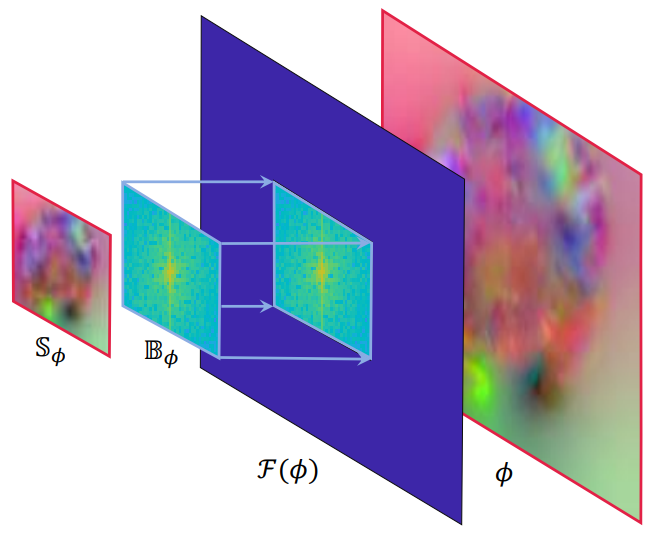
\includegraphics[width=.65\linewidth]{DecoderDisplacementField.png} 
	\caption{Reconstruction of the displacement field via the decoder taken from~\cite{Fourier-Net+}.}
	\label{fig:DecoderDisplacementField}
\end{figure} 

\subsection{Diffeomorphic Transforms} \label{SubSec:DiffeomorphicTransforms}
Diffeomorphic deformations are differentiable and invertible, thus preserving topology, which is a desirable property for transformations. $\phi: \mathbb{R}^N \rightarrow \mathbb{R}^N$ represents the deformation that maps the coordinates from one image to coordinates in another image, as long as both images have the dimension $N$. When using a stationary velocity field representation like e.g. \emph{DARTEL}~\cite{DARTEL}, the deformation field is defined through the following ordinary differential equation (ODE)~\cite{Dalca2018}:
\begin{equation}
	\frac{\partial \phi^{(t)}}{\partial t} = v(\phi^{(t)}),
\end{equation}
where $\phi^{(0)} = \text{Id}$ is the identity transformation and $t$ is time. The final registration field $\phi^{(1)}$ can be obtained by integrating the stationary velocity field $v$ over $t = [0, 1]$. This is typically done by integration numerically using scaling and squaring~\cite{ScaleAndSquare}. The integration of a stationary ODE represents a one-parameter subgroup of diffeomorphisms. In group theory, $v$ is a member of the Lie algebra and is exponentiated to produce $\text{exp}(v) = \phi^{(1)}$, which is also a member of the Lie group. From the properties of one-parameter subgroups, for any scalars $t$ and $t'$, $\text{exp}((t + t') \cdot v) = \text{exp}(t \cdot v) \circ \text{exp}(t' \cdot v)$, where $\circ$ is a composition map associated with the Lie group. Starting from $\phi^{({1/2}^T)} = p + v(p)$ where $p$ is a map of spatial locations, we use the recurrence $\phi^{({1/2})^{t−1}} = \phi^{({1/2}^t)} \circ \phi^{({1/2}^t)}$ to obtain $\phi^1 = \phi^{(1/2)} \circ \phi^{(1/2)}$. $T$ is chosen so that $v \approx 0$~\cite{Dalca2018}. \\
As diffeomorphic deformations are defined as smooth and invertible deformations, the output of the iDFT layer in \emph{Fourier-Net} can be regarded as a stationary velocity field $v$ instead of a displacement field $\phi$. In Figure~\ref{fig:Fourier-Net} scaling and squaring layers are visualized. These apply the diffeomorphic transformation in three steps~\cite{ScaleAndSquare}:
\begin{enumerate}
	\item Scaling: Divide the velocity field $v$ by a factor $2^N$ , so that $\frac{v}{2^N}$ is close to zero (depending on the desired accuracy).
	\item Exponentiation: Compute $\text{exp}\big(\frac{v}{2^N}\big) = \phi^{(1)}\big(\frac{v}{2^N}\big)$ with a first-order explicit numerical scheme.
	\item Squaring: $N$ recursive squarings of $\phi^{(1)}\big(\frac{1}{2^N}\big) = \text{exp}\big(\frac{v}{2^N}\big)$ to yield an accurate estimation of $\phi^{(1)}(1) = \phi^{(1)}\big(\frac{1}{2^N}\big)^{2^N} = \text{exp}\big(\frac{v}{2^N}\big)^{2^N} = \text{exp}(v)$.
\end{enumerate}
Thus, the diffeomorphic deformation can be efficiently calculated. When used, the specific version is then called \emph{Fourier-Net Diff} to differentiate it from the baseline version.


\subsection{Spatial Transformer} \label{SubSec:SpatialTransformer}
The warping layer of \emph{Fourier-Net} utilizes the \emph{Spatial Transformer}~\cite{SpatialTransformer}, which allows for spatial image manipulation within the network. This is a differentiable and learnable module for neural networks which applies a spatial transformation to a feature map during a single forward pass. The spatial transformer mechanism is split into three parts as seen in Figure~\ref{fig:SpatialTransformer}. First is the localization network, which takes the input and outputs the parameters for the transformation. These are then used to create a sample grid using the grid generator. Lastly, the sampler produces the output feature map based on the input at the grid points.\\
From the input feature map $U \in \mathbb{R}^{H \times W \times C}$ with width $W$, height $H$ and channels $C$ the localization network $f_{\text{loc}}$ computes the parameters $\theta = f_{\text{loc}}(U)$ of the transformation $\mathcal{T}_\theta$ which is later applied to the feature map. Thus the size of $\theta$ varies depending on the transformation. 
%(e.g. 6D for an affine transformation). 
The localization network function can both be implemented as a fully-connected network or as a CNN, but should include a final regression layer to produce the transformation parameters.\\
In order to warp the input feature map, each output pixel is computed by applying a sampling kernel centered at a particular location in the input feature map. The output pixels are defined to lie on a regular grid $G = {G_i}$ of pixels, forming an output feature map $V \in \mathbb{R}^{H' \times W' \times C}$, where $H'$ and $W'$ are the height and width of the grid with C again being the number of channels, which is the same for input and output.\\
In order to perform a spatial transformation of the input feature map $U$, the sampler must take the set of sampling points $\mathcal{T}_\theta(G)$, along and produce the sampled output feature map $V$. Each coordinate $(x_i^s, y_i^s)$ in $\mathcal{T}_\theta(G)$ defines the spatial location in the input where a sampling kernel is applied to get the value at a particular pixel in the output:
\begin{equation}
	V_i^c = \sum^{H}_{n} \sum^{W}_{m} U_{nm}^c k(x_i^s - m; \Phi_x) k(y_i^s - n; \Phi_y),
\end{equation}
with $\Phi_x$ and $\Phi_y$ being the parameters for a generic sampling  kernel $k$ that defines the image interpolation, $U_{nm}^c$ is the value of the input feature maps at location $(n,m)$ in the channel $c \in [1, ..., C]$ and $V_i^c$ is the value for every pixel $i \in [1, ..., H'W']$ for the output feature map. Any sampling kernel can be used, as long as (sub-) gradients can be defined with respect to $(x_i^s, y_i^s)$ to allow the loss gradients to flow back not only to the input feature map, but also to the sampling grid coordinates and therefore back to the transformation parameters $\theta$ and localization network, thus enabling back-propagation~\cite{SpatialTransformer}.
\begin{figure}[htpb]
	\centering
	\graphicspath{{images/}{\main/images/}}
	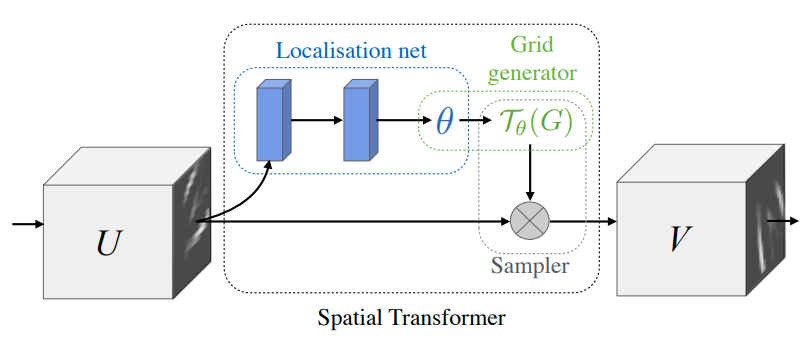
\includegraphics[width=\linewidth]{SpatialTransformer.png} 
	\caption{Architecture of the \emph{Spatial Transformer} taken from~\cite{SpatialTransformer}.}
	\label{fig:SpatialTransformer}
\end{figure}


\subsection{Loss Function} \label{SubSec:LossFunction}
The loss function consists of two parts to enable unsupervised learning, which are balanced using the scalar parameter $\lambda$. The first, $\mathcal{L}_{1}$, measures the similarity between the fixed image and the moving image after warping, while the second, $\mathcal{L}_{2}$, ensures a smooth displacement field. Thus, the unsupervised loss $\mathcal{L}$ can be calculated as follows:
\begin{equation}	\label{eq:unsupervisedLoss}
	\begin{split} 
		\mathcal{L}(\Theta) &= \min  \bigg( \mathcal{L}_{1} (\phi(\Theta))  + \lambda \cdot \mathcal{L}_{2} (\phi(\Theta)) \bigg) \\
		&= \min  \bigg( \mathcal{L}_{1} (v(\Theta))  + \lambda \cdot \mathcal{L}_{2} (v(\Theta)) \bigg),
	\end{split}
\end{equation}
for both displacement fields $\phi$ and velocity fields $v$. The first part of the loss function consists of:
\begin{equation} \label{eq:L1-LossDisp}
	\mathcal{L}_{1} (\phi(\Theta)) = \frac{1}{N} \sum^{N}_{i=1} \mathcal{L}_{Sim} (M_i \circ (\phi_i(\Theta) + \text{Id}) - F_i),
\end{equation}
where $\circ$ denotes the warping operation, $N$ the number of training pairs with moving images $M_i$ and fixed images $F_i$, $\Theta$ the network parameters, $\phi_i$ the displacement field, Id the identity grid. $\mathcal{L}_{Sim}$ determines the similarity between warped moving images and fixed images via MSE or NCC, and the second term of the unsupervised loss, $\mathcal{L}_{2}$, defines the smoothness regularization function that controls smoothness of the displacement fields:
\begin{equation} \label{eq:L2-LossDisp}
	\mathcal{L}_{2} (\phi(\Theta)) = \frac{1}{N} \sum^{N}_{i=1} || \nabla \phi_i(\Theta) ||^2_2,
\end{equation}
with $\nabla$ denoting the first order gradient and $|| \cdot ||_2^2$ denoting the squared $L_2$-Norm. \\
When using the squaring and scaling layers, thus making the deformation of the moving image diffeomorphic, the loss needs to be modified by replacing the displacement field $\theta$ with the velocity field $v$. Thus, both parts of the of the loss function need to be changed:
\begin{equation}	\label{eq:L1-LossVeloc}
	\mathcal{L}_{1} (v(\Theta)) = \frac{1}{N} \sum^{N}_{i=1} \mathcal{L}_{Sim} (M_i \circ Exp(v_i(\Theta) - F_i),
\end{equation}
\begin{equation} \label{eq:L2-LossVeloc}
	\mathcal{L}_{2} (v(\Theta)) = \frac{1}{N} \sum^{N}_{i=1} || \nabla v_i(\Theta) ||^2_2  \bigg .
\end{equation}

% Should go into Chapter Experiments, but is unimportant anyway...
%\subsection{Training on OASIS}
%We first trained \emph{Fourier-Net} and \emph{Fourier-Net+} with the \emph{OASIS} dataset, as it was used in the original publication. \emph{Fourier-Net}/\emph{Fourier-Net+} can work with both 2D and 3D inputs, however the latter are harder to visualize. As the \emph{OASIS} dataset provides 3D volumes with annotations, 2D image data can be obtained by slicing the 3D volumes (see Figure~\ref{fig:OASIS} with matching labels for Dice-Score calculation. Thus we can easily visualize the training success of the 2D network by looking at the difference between images before and after registration in addition to the Dice-Score, which can also be calculated for 3D data. Examples for this can be seen in Figure~\ref{fig:DifferencesTrainingProgress} with two examples from different stages of the training process. Despite the example in Figure~\ref{fig:Training29600it} being the far harder example to align the network performs better than before (see Figure~\ref{fig:Training800it}) due to the training progress.
%
%\begin{figure}[htpb]
%	\centering
%	\graphicspath{{images/}{\main/images/}}
%	\begin{subfigure}{0.45\textwidth}
%		\centering
%    		\includegraphics[width=\textwidth]{results1.png}
%    		\caption{Training progress after 800 iterations.}
%    		\label{fig:Training800it}
%	\end{subfigure}
%	\hfill
%	\begin{subfigure}{0.45\textwidth}
%		\centering
%    		\includegraphics[width=\textwidth]{results2.png}
%    		\caption{Training progress after 29600 iterations.}
%    		\label{fig:Training29600it}
%	\end{subfigure}
%	\caption{Differences between moving and fixed images before and after registration.}
%	\label{fig:DifferencesTrainingProgress}
%\end{figure}
%
%\subsection{Training on CMRxRecon}
%For the further experiments we used the \emph{CMRxRecon} dataset. We reconstructed 2D images and trained the network similar to the \emph{OASIS} dataset.

\section{Fourier Net+} \label{Sec:Fourier-Net+}
\emph{Fourier-Net+}, as the name suggests, is an extension of Fourier-Net which takes the band-limited spatial representation of the images as input, instead of their original full-resolution counterparts. This leads to further reduction in the number of convolutional layers in the contracting path of the network, resulting in a decrease of parameters, memory usage, and computational operations. This makes \emph{Fourier-Net+} even more efficient than its predecessor~\cite{Fourier-Net+}.\\
As seen in Figure~\ref{fig:Fourier-Net+}, the network architecture is almost the same as for \emph{Fourier-Net} (see Figure~\ref{fig:Fourier-Net} for comparison). However, while the decoder, and thus the loss function, remain the same, the encoder is slightly altered to make the network even more efficient. For this, similarly to the decoder, a DFT is used, however this time the idea is applied to the input images. These are first transformed into the Fourier domain, then low-pass filtered by center-cropping and finally reconstructed from their band-limited representation back into the spatial domain via an iDFT. The two images, now compressed, are the input for the encoder of \emph{Fourier-Net}, meaning the CNN and following DFT. However, due to the band-limiting before the CNN, the latter can be made much more light-weight, thus reducing computational cost. This is visualized in Figure~\ref{fig:Fourier-Net+CNN}. Thus, \emph{Fourier-Net+} too is overall lighter than the baseline \emph{Fourier-Net} in terms of the number of parameters and computations. However, such a light network may face limitations in accurately capturing complex deformations. To counter this potential weakness, the authors propose a cascaded version of \emph{Fourier-Net+}, which uses multiple versions of \emph{Fourier-Net+} cascaded one after the other to achieve a better overall displacement field~\cite{Fourier-Net+}. A schematic for this can be seen in Figure~\ref{fig:Fourier-Net+Cascaded}.

\begin{figure}[htpb]
	\centering
	\graphicspath{{images/}{\main/images/}}
	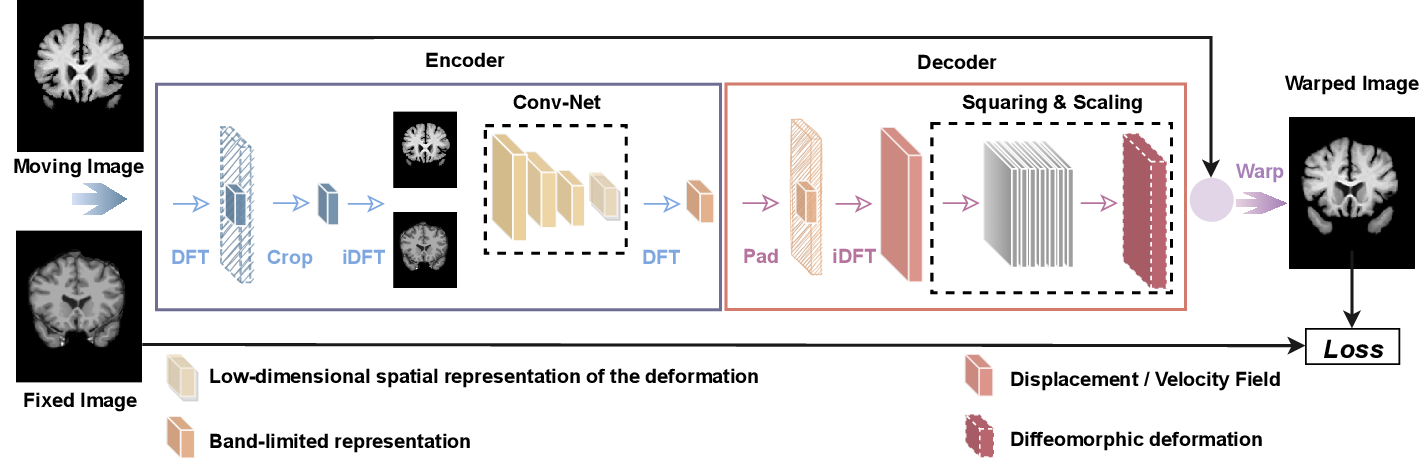
\includegraphics[width=\linewidth]{ArchitectureFourier-Net+.png} 
	\caption{Architecture of \emph{Fourier-Net+} taken from~\cite{Fourier-Net+}.}
	\label{fig:Fourier-Net+}
\end{figure}

\subsection{Changes to the Encoder} \label{SubSec:ChangesEncoder}
In order to further reduce the amount of computational operations, \emph{Fourier-Net+} discards the early layers of the encoder. Instead, a DFT $\mathcal{F}(I_M)$ followed by a center-crop to produce the band-limited representation $\mathbb{B}_{I_M}$ in the frequency domain and iDFT are used to get the spatial patch $\mathbb{S}_{I_M}$, while the rest of the encoder from \emph{Fourier-Net} stays the same. The input $I_M$ is thus compressed to a lower resolution (i.e. band-limited) using the frequency space, which reduces the computational cost. This process is visualized in Figure~\ref{fig:Fourier-Net+EncoderCompression}. The encoder of \emph{Fourier-Net+} has several convolutional layers less in the contracting path compared to \emph{Fourier-Net}, which leads to a further accelerated registration process while reducing the memory footprint. These advantages are visualized in Figure~\ref{fig:Fourier-Net+CNN} where the amount of different layers between a conventional \emph{U-Net}, \emph{Fourier-Net} (with the smaller decoder) and \emph{Fourier-Net+} (with a smaller encoder and decoder) are shown.
\begin{figure}[htpb]
	\centering
	\graphicspath{{images/}{\main/images/}}
	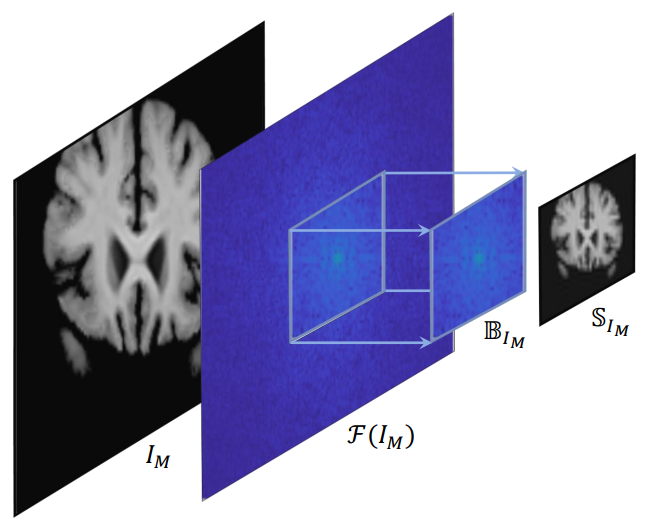
\includegraphics[width=.5\linewidth]{CompressionEncoder.png} 
	\caption{Compression in the frequency domain of the encoder used in \emph{Fourier-Net+} taken from~\cite{Fourier-Net+}.}
	\label{fig:Fourier-Net+EncoderCompression}
\end{figure}
\begin{figure}[htpb]
	\centering
	\graphicspath{{images/}{\main/images/}}
	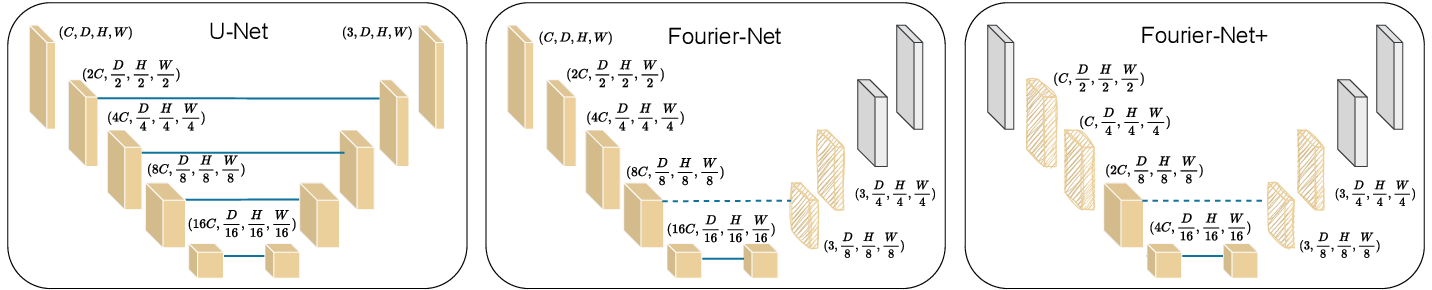
\includegraphics[width=\linewidth]{ArchitectureFourier-Net+CNN.png} 
	\caption{Architecture of the CNN for a typical U-Net, \emph{Fourier-Net} and \emph{Fourier-Net+} taken from~\cite{Fourier-Net+}.}
	\label{fig:Fourier-Net+CNN}
\end{figure}

\subsection{Effects of Cascading} \label{SubSec:EffectsCascading}
As seen in the previous section, \emph{Fourier-Net+} is lighter than \emph{Fourier-Net} due to the band-limited representation of both images and deformations lowering the number of parameters and computations. This, however, can lead to limitations when trying to accurately capture complex deformations. To this end, a cascaded version of \emph{Fourier-Net+} called \emph{K$\times$Fourier-Net+} (see Figure~\ref{fig:Fourier-Net+Cascaded}), with $K$ denoting the amount of cascades, can be used where the the warped image of one cascade is used as the moving image of the next. It is important to note that the weights are not shared between cascades. The squaring and scaling layers, in case a diffeomorphic deformation is wanted, are applied after the last cascade. The same is true for the calculation of the loss function.\\
In order to more accurately describe this version of \emph{Fourier-Net+} one can look at the in- and outputs of the different cascades. The first cascade of \emph{K$\times$Fourier-Net+} has the moving image $I_M$ and fixed image $I_F$ as inputs. While the latter always stays the same for all cascades the warped image $I_M^{w(1)}$ from the first cascade is used as input for the second cascade instead of the original moving image. Thus, in general $I_M^{w(k-1)}$ and $I_F$ are the inputs for a cascade $k \in [1, K]$ with output $\delta \phi^{(k)}$. Furthermore, $I_M^{w(k)}$ can be defined as:
\begin{equation}
	I_M^{w(k)} = ((((I_M \circ \delta \phi^{(1)}) \circ \delta \phi^{(2)}) \circ \dots ) \circ \delta \phi^{(k-1)}) \circ \delta \phi^{(k)} = I_M \circ  \phi^{(k)},
\end{equation}
with $\phi^{(k)}$ being the displacement field computed by composing the outputs of the first cascade up to the $k$-th cascade:
\begin{equation}
	\phi^{(k)} = \delta \phi^{(1)} \circ \delta \phi^{(2)} \circ \dots \circ \delta \phi^{(k-1)} \circ \delta \phi^{(k)}.
\end{equation}
Thus, the output displacement field of the $K$-th cascade $\phi^{(K)}$ is the final displacement which is then used to warp $I_M$, the original moving image, in order to compute the loss~\cite{Fourier-Net+}.

\begin{figure}[htpb]
	\centering
	\graphicspath{{images/}{\main/images/}}
	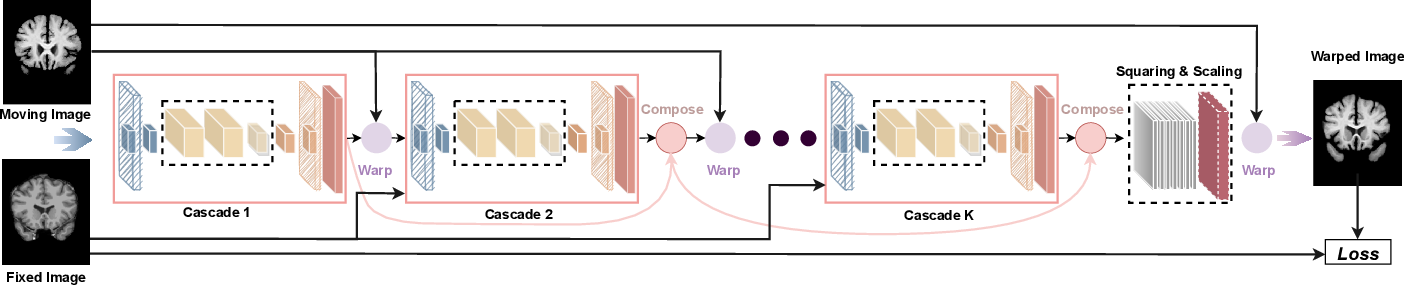
\includegraphics[width=\linewidth]{ArchitectureFourier-Net+Cascaded.png} 
	\caption{Cascaded version of \emph{Fourier-Net+} taken from~\cite{Fourier-Net+}.}
	\label{fig:Fourier-Net+Cascaded}
\end{figure}

\chapter{Experiments} \label{Ch:Experiments}
In the following chapter the different experiments that were conducted are described and explained. 
%First was frame-to-frame registration on cardiac data from the \emph{CMRxRecon} dataset to lay the basis for later experiments with a motion-correcting reconstruction pipeline.
First, experiments were conducted on the \emph{CMRxRecon} dataset to find the optimal parameters for our model. As this dataset lacks ground truth segmentations, the \emph{ACDC} dataset was used to extend these tests.


\section{Parameter Studies on the CMRxRecon Dataset} \label{Sec:ParameterStudies}
As a first step, frame-to-frame registration on the \emph{CMRxRecon} dataset was tested. The goal of these initial experiments was to examine whether the network could learn to align the cardiac image pairs despite the movement between the frames. To start, different parameters were tested in order to find the optimal model parameters for the \emph{CMRxRecon} dataset. 
%This would hopefully form the basis to use the networks in a motion-corrected reconstruction pipeline later. 
\\
As discussed in section~\ref{SubSec:Pre-Processing}, the CMR images were cropped to extract the moving cardiac region. This was done for both the fully sampled and subsampled (Acc4, Acc8, Acc10) data. Image pairs for each slice from each patient of the training set were generated to train the network. In order to evaluate the training progress the mean MSE and mean SSIM metrics calculated the validation data at each checkpoint (usually every 1000 iterations). The best model parameters, as determined by the metrics, were saved in a separate folder. To further evaluate the training success the unseen test data containing new patients was used. To benchmark the networks training success the MSE and SSIM were again used, but the mean inference time and the percentage of non-positive Jacobian determinant of deformation ($\% \, |J_{\phi}|\leq0$) were also calculated. The procedure, however, was slightly altered for the subsampled data as only the displacement field of the model was used to align the corresponding fully sampled image pairs. The evaluation metrics were then calculated on these images for better comparability.

\subsection{Fourier-Net versus Fourier-Net+} \label{SubSec:Fourier-NetvsFourier-Net+}
First, the baseline network \emph{Fourier-Net} was compared to its newer version \emph{4xFourier-Net+} once with both using the diffeomorphic version and once without the transform. Thus the effect of the diffeomorphic deformation can be compared to the normal transformation on \emph{Fourier-Net} and \emph{4xFourier-Net+}. All of the experiments were conducted on the fully sampled data as the subsampling should not effect the tested properties. The other parameters were also kept constant with a learning rate of $0.0001$, MSE-loss and $\lambda = 0.01$. FT crop in \emph{4xFourier-Net+} was set to $24 \times 24$.


\subsection{Starting Channel Size} \label{SubSec:StartingChannels}
Next, the impact of the starting channels was examined. For this, \emph{4xFourier-Net+} was trained with MSE-loss, a learning rate of $0.0001$, $\lambda = 0.01$, FT crop of $24 \times 24$ and no diffeomorphic transform. The experiments were again only conducted on the fully sampled data. Three different channel sizes were used for training \emph{Fourier-Net+}: $8$, $16$ and $32$. Due to the early stopping the networks were trained for 17, 17 and 10 epochs respectively. 
%\\Similarly, \emph{Fourier-Net} was tested with the same parameters for channel sizes $8$, $16$ and $32$. These were trained for y epochs.


\subsection{Quantitative Comparison with NiftyReg} \label{SubSec:QuantitativeComparisonNiftyReg}
To establish a baseline, the similarity metrics were calculated between the unaligned test data. \emph{4xFourier-Net+} was then trained with the MSE-loss, 8 channels, $\lambda = 0.01$ and a learning rate of $0.0001$. \emph{NiftyReg}, a traditional registration algorithm that iteratively optimizes the displacement~\cite{NiftiReg}, was used for comparison. \emph{NiftyReg} provides the warped image for the fully sampled data directly, but for the subsampled data the control point grid produced by \emph{NiftyReg} was used to resample the corresponding fully sampled data for comparability. Thus only the fully sampled test data is needed for an unregistrated baseline as the subsampled data is only used to produce the displacement which is then used to warp the fully sampled data. 
%The MSE of the registration methods should thus not exceed  $0.000535$ and the SSIM should be higher than $0.91714$.


\section{Parameter Tests on the ACDC Dataset}
As the evaluation on the \emph{CMRxRecon} dataset is limited to image similarity measures, further testing was done on the \emph{ACDC} dataset which contains cardiac data with segmentations. These can be used to better evaluate the registration performance by using e.g. the Dice score.


\subsection{Fourier-Net versus Fourier-Net+} \label{SubSec:Fourier-NetvsFourier-Net+}
First, \emph{Fourier-Net}, \emph{Fourier-Net+} and \emph{4xFourier-Net} are compared for both normal and diffeomorphic versions. Additionally, network versions creating dense instead of band-limited displacements were used a baseline for the best achievable performance. The registration performance was evaluated on the test set using the percentage of Dice scores calculated with and without the background label, percentage of SSIM, MSE multiplied by $10^-3$ (denoted by m for milli) and the percentage of negative Jacobian determinant of deformation. The mean inference time on the GPU together with memory consumption for each model are also added to the comparison with the latter containing number of trainable model parameters, mult-add operations (in millions or billion as denoted by M or G) and the total memory in Megabyte (MB). The latter is only given for the normal versions as the diffeomorphic version require the same amount of memory as well as the baseline dense versions. The first network was trained for a maximum of 15 epochs with early stopping activating after 3 epochs without improvement of the validation Dice score. The other variants were than trained with the same number of epochs, which worked out to be only 6 epochs due to the large training set in the experiments without any data augmentation. All networks were trained on the fully sampled \emph{ACDC} data with MSE as the unsupervised similarity loss, a channel size of 8, learning rate of 0.0001 and $\lambda=0.01$. \emph{Fourier-Net+} and \emph{4xFourier-Net} used a FT crop size of $48 \times 48$ for these experiments. All of these parameters were constant for the diffeomorphic and dense versions of the networks. The results and subsequent discussion can be found in section~\ref{SubSec:ResultsFourier-NetvsFourier-Net+ACDC}.


\subsection{Starting Channel Size} \label{SubSec:StartingChannelsACDC}
Next, the impact of the starting channels on the \emph{ACDC} data was examined as these dictate the number of features that the network uses. For this, \emph{Fourier-Net+} and \emph{4xFourier-Net+} was trained with MSE-loss, a learning rate of $0.0001$, $\lambda = 0.01$, FT crop of $24 \times 24$ and no diffeomorphic transform. The experiments were again only conducted on the fully sampled data. Four different channel sizes were used for training: $8$, $16$, $32$ and $64$. The first network variant was trained with early stopping, which ended at 6 epochs. For better comparability, the other network variants were also trained with the same number of epochs. The registration performance was evaluated on the test set using the percentage of the Dice score calculated once on all labels, once without the background using only the cardiac labels, as well as the percentage of SSIM, MSE multiplied by $10^-3$ and the percentage of negative Jacobian determinant of deformation. Additionally the number of network parameters, number of mult-add operations (in millions or billion as denoted by M or G) and memory consumption in Megabyte (MB) are listed for all network variants to better compare the relationship between registration performance and memory consumption to potentially find a optimal configuration for both performance and efficiency. The mean inference time was measured on GPU in seconds. The results and subsequent discussion can be found in section~\ref{SubSec:ResultsStartingChannelsACDC}.


\subsection{Fourier-Transform Crop Size} \label{SubSec:FTCropSize}
The FT crop size, used for compressing the input images, is a parameter specific to \emph{Fourier-Net+} and \emph{4xFourier-Net+}. Four different sizes of the FT crop were analyzed: $80 \times 168$, $40 \times 84$, $48 \times 48$ and $24 \times 24$. A larger crop would obviously compress the images less, thus leading to less efficiency, however, a very small crop, while very efficient, might lose some of the image details leading to a decrease in performance. The experiments were again only conducted on the fully sampled data as one would expect similar results on subsampled data. The network variants were trained with MSE as the unsupervised similarity loss, a channel size of 8, learning rate of 0.0001 and $\lambda=0.01$. Again, the networks were trained for only 5 epochs, as this is were the first model ended training due to early stopping. The registration performance was evaluated on the test set using the Dice score calculated once on all labels, once without the background, as well as the SSIM, MSE and the percentage of negative Jacobian determinant of deformation. Additionally, the number of network parameters, number of mult-add operations in millions (M) and memory consumption in Megabyte (MB) are listed for all network variants to better compare the relationship between registration performance and memory consumption to potentially find a optimal configuration for both performance and efficiency. The mean inference time was measured on GPU in seconds. The results and subsequent discussion can be found in section~\ref{SubSec:ResultsFTCropSize}.


\subsection{Comparison with VoxelMorph} \label{SubSec:ComparisonVoxelMorph}
After finding parameters which optimize registration performance while trying to minimize memory consumption, a comparison to another commonly used registration network should be made. For this, the famous \emph{VoxelMorph}~\cite{Voxelmorph} was used. It was trained with the default number of layers, MSE as the similarity loss, a learning rate of 0.0001, $\lambda=0.01$ and provides a dense displacement field to align the image pair. For comparison \emph{Fourier-Net}, \emph{Fourier-Net+} and \emph{4xFourier-Net+} were trained for 6 epochs with MSE as the unsupervised similarity loss, a channel size of 16, learning rate of 0.0001 and $\lambda=0.01$ as well as a FT crop size of $48 \times 48$, which provide a good balance of performance and memory imprint for the networks. To evaluate registration performance, the Dice score was again computed for all labels and without the background as well as the similarity metrics SSIM, MSE and the percentage of negative Jacobian determinant of deformation. All networks were trained on the fully sampled \emph{ACDC} data. The inference times of all networks were computed on the GPU and the number of network parameters, number of mult-add operations in billions (G) and memory consumption in Megabyte (MB) are also given to further compare the efficiency of the networks. 


\subsection{Dense Displacement on Accelerated Data} \label{SubSec:DenseDisplacementAcc}
The difference between a dense displacement field and a band-limited one was already explored in section~\ref{SubSec:Fourier-NetvsFourier-Net+}. This, however, only includes fully sampled data, not accelerated data. This section explores potential performance changes on the latter with the hypothesis that the network variants with the dense displacement will perform worse than the variants with the band-limited displacement field for strongly subsampled data. This expectation stems from the fact that frequencies outside the center region of the k-space are dropped for the accelerated data thus reducing the advantage of the dense displacement in comparison to the band-limited (i.e. center-cropped) displacement. \\
The tests again included \emph{Fourier-Net}, \emph{Fourier-Net+} and \emph{4xFourier-Net+}, which were all trained for 6 epochs with MSE as the unsupervised similarity loss, a channel size of 16, learning rate of 0.0001 and $\lambda=0.01$. The registration performance was evaluated on the test set using the Dice score calculated once on all labels, once without the background, as well as the SSIM, MSE and the percentage of negative Jacobian determinant of deformation. Additionally, the number of network parameters, number of mult-add operations in millions (M) and memory consumption in Megabyte (MB) are given.

\subsection{Comparison on Subsampled Data} \label{SubSec:ComparisonSubsampling}
After comparing \emph{Fourier-Net}, \emph{Fourier-Net+} and \emph{4xFourier-Net+} with both dense and band-limited displacement fields as well as another comparison with \emph{VoxelMorph} on fully sampled data 
%to access the difference in registration performance and memory consumption 
an extension to subsampled data needs to be made. For this \emph{Fourier-Net}, \emph{Fourier-Net+} and \emph{4xFourier-Net+} were compared to a baseline consisting of the unaligned test image pairs as well as \emph{NiftyReg}, \emph{VoxelMorph} and \emph{LAPNet}. Thus, observations of the performance on accelerated data can be made as well as comparisons to the aligned baseline (which all methods should aim to beat), a traditional registration algorithm, a dense registration network working in the image domain and a another dense network which works in the k-space domain.\\
\emph{Fourier-Net}, \emph{Fourier-Net+} and \emph{4xFourier-Net+} were trained for 6 epochs with MSE as the unsupervised similarity loss, a channel size of 16, learning rate of 0.0001 and $\lambda=0.01$ as well as a FT crop size of $48 \times 48$ for all subsampling data. VoxelMorph was trained with default layers and MSE as the similarity loss, a learning rate of 0.0001 and $\lambda=0.01$. Three different accelerations were tested: \textit{Acc4} (R=4), \textit{Acc8} (R=8) and \textit{Acc10} (R=10). For reference, the data for the fully sampled data (R=0) is also provided. The registration performance of all methods was evaluated on the test set using the Dice score calculated once on all labels, once without the background, as well as the SSIM and MSE as image metrics. All times are computed on CPU for better comparability as \emph{NiftyReg} currently only works on CPU as the GPU capable versions were deprecated and the other networks would gain an unfair time advantage when ran on GPU. The baseline obviously has no time associated as it only denotes the metrics on the test data before registration. The results and an comprehensive discussion are provided in section~\ref{SubSec:ResultsComparisonSubsampling}.


\section{Data Consistency Experiments and Network Changes}
In this section, changes to the network architecture and loss function are discussed.

\subsection{Data Consistency Loss}
As seen in the section~\ref{SubSec:ResultsComparisonSubsampling}, the performance for all methods decreases drastically for highly subsampled/accelerated data due to reconstruction artifacts in the image domain due to the missing frequencies in the k-space domain. However, since we are interested in maintaining performance on subsampled data, it might prove useful to use k-space information for the loss calculation and thus for the network training as it should not contain artifacts compared to the image domain. Thus, it would act as a kind of data consistency contraint during training. In order to achieve this, the similarity loss for \emph{Fourier-Net}, \emph{Fourier-Net+} and \emph{4xFourier-Net+} was calculated not on the warped and fixed images, but instead on their corresponding masked k-spaces. This would hopefully still provide the network with useful information during training that is free of any aliasing artifacts, which might decrease performance on subsampled data. The k-spaces were masked to only compare the sampled frequencies to avoid large differences between the deleted frequencies of the fixed image with potential interpolated frequencies of the warped image. \\
After trying the MSE as the similarity loss, it quickly became apparent that this yielded wildly inconsistent displacements which often corrupted the warped image and could no longer be reigned in by the smoothness constraint of the loss function. Even with a $\lambda = 10$ to put a greater emphasize on the smoothness of the displacement, unrealistic deformations could not be prevented as the training did not appear to converge.

%\subsection{Changes to the Network Architecture}
%Next, a change to the network architecture was tested that changed the domain from image to k-space in hopes of avoiding the reconstruction artifacts present in highly accelerated images. For this we first looked at \emph{LAPNet} which works on k-space data, but is trained in a supervised manner. As a first test, we tried to train it in an unsupervised method with the same pipeline as \emph{Fourier-Net}. To achieve this we needed to generate $33 \times 33$ crops of the k-spaces as LAPNet iteratively predicts the displacement for the center-pixel of each crop, thus producing a dense displacement for the whole image.

\section{Integration into a Motion-Corrected Reconstruction Pipeline} \label{Sec:IntegrationMotion-CorrectedReconstructionPipeline}
Describe qualitative test to see whether the network can be used to improve a reconstruction pipeline for cardiac data.


\subsection{General Reconstruction Pipeline}
Overview of the reconstruction pipeline using \emph{Fourier-Net+}.

\begin{figure}[htpb]
	\centering
	\graphicspath{{images/}{\main/images/}}
	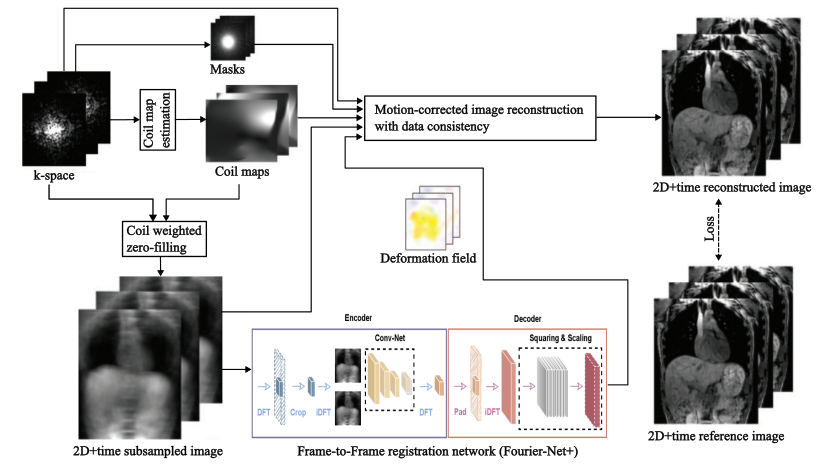
\includegraphics[width=\linewidth]{ReconstructionPipelineCompact.png} 
	\caption{Overview of the general reconstruction pipeline using \emph{Fourier-Net+} as a registration network.}
	\label{fig:ReconstructionPipeline}
\end{figure}


%%%%%%%%%%%%%%%%%%%%%%%%%%%%
%% Results and Discussion %%
%%%%%%%%%%%%%%%%%%%%%%%%%%%%

\chapter{Results and Discussion} \label{Ch:ResultsDiscussion}
In this chapter, the results for the experiment described in the previous chapter will be examined. Possible implications will be discussed to determine the effectiveness of this new method.

%\section{Frame-to-Frame Registration} \label{Sec:Frame-to-FrameRegistration}
%As mentioned in section~\ref{Sec:Frame-to-Frame_CMRxRecon}, frame-to-frame registration on the \emph{CMRxRecon} dataset was the first set of experiments. Goal of these initial tests was to examine whether the network could learn to align the cardiac image despite the movement between the frames. 


\section{Parameter Studies on the CMRxRecon Dataset} \label{Sec:ParameterStudies}
Different parameters were tested in order to find the optimal model parameters for usage on the \emph{CMRxRecon} dataset. After some tests on the fully sampled data, a comparison with the traditional iterative algorithm \emph{NiftyReg} was conducted on both the fully sampled and subsampled data.

\subsection{Fourier-Net versus Fourier-Net+} \label{SubSec:ResultsFourier-NetvsFourier-Net+CMRxRecon}
First, the baseline network \emph{Fourier-Net} was compared to its more efficient successor \emph{4xFourier-Net+} with both using the diffeomorphic version as we can then compare the effect of the diffeomorphic deformation compared to the normal transformation on \emph{4xFourier-Net+}. However, this effect should be similar for \emph{Fourier-Net}. All of the experiments were conducted on the fully sampled data as the subsampling should not effect the tested properties. The baseline MSE (note that all MSE values are multiplied by $10^-3$ as denoted by the m) for unregistrated test images is $0.535$ and the SSIM percentage ($\%$ SSIM) is $91.71$. The results for \emph{Fourier-Net} and \emph{4xFourier-Net+} can be seen in Table~\ref{tab:Fourier-NetvsFourier-Net+CMRxRecon}. \\
The \emph{Fourier-Net} model without the diffeomorphic transform was trained for 17 epochs, while the diffeomorphic version trained for 100 epochs. Despite this, the latter is only marginally better in terms of MSE and SSIM. The percentage of negative Jacobian determinants was actually better for the normal transformation compared to the diffeomorphic one. The normal \emph{Fourier-Net+} model trained for 37 epochs, while the diffeomorphic version trained for 100 epochs. \emph{Fourier-Net+} performs slightly worse than \emph{Fourier-Net}, however it is more efficient.


\begin{table}[htpb]
	\centering
	\caption{Results for \emph{Fourier-Net} and \emph{Fourier-Net+} on the fully sampled \emph{CMRxRecon} test data with a diffeomorphic transform.}
	\label{tab:Fourier-NetvsFourier-Net+CMRxRecon}
	\begin{tabular}{c c c c c} %
		\toprule
		Model & MSE (m) & $\%$ SSIM & $\% \, |J_{\phi}|\leq0$ & Time [s] \\
		\midrule
		Fourier-Net & $0.319 \pm 0.352$ &  $93.29 \pm 3.85$ & $0.0022 \pm 0.0183$ & 0.0025\\ 
		4xFourier-Net+ & $0.352 \pm 0.449$ & $93.08 \pm 4.09$ & $0.0003 \pm 0.0057$ & 0.0123\\ 
		\midrule
		Diff-Fourier-Net & $0.318 \pm 0.388$ &  $93.39 \pm 3.82$ & $0.0273 \pm 0.0897$ & 0.0028\\ 
		Diff-4xFourier-Net+ & $0.352 \pm 0.448$ & $93.08 \pm 4.11$ & $0.0029 \pm 0.0214$ & 0.0103\\  
		\bottomrule
	\end{tabular}
\end{table}


\subsection{Starting Channel Size} \label{SubSec:ResultsStartingChannelsCMRxRecon}
Next, the impact of the starting channels was examined. For this, \emph{4xFourier-Net+} was trained with three different channel sizes: $8$, $16$, $32$ and $64$. 
%Due to the early stopping the \emph{Fourier-Net} variants were trained for 17, x, x and x epochs, while the channel sizes: $8$, $16$, $32$ and $64$. 
Due to the early stopping the \emph{4xFourier-Net+} variants were trained for x, 17 and 10 epochs respectively. The results can be seen in Table~\ref{tab:StartingChannelsFourierNet+CMRxRecon} with the inference time for each version being calculated on the GPU.
% and~\ref{tab:StartingChannelsFourierNet}. 
Despite training for the least amount of epochs channel size $32$ performs the best for \emph{4xFourier-Net+}.

\begin{table}[htpb]
	\centering
	\caption{Results for three different starting channel sizes of  \emph{Fourier-Net+} on the fully sampled \emph{CMRxRecon} test data.}
	\label{tab:StartingChannelsFourierNet+CMRxRecon}
	\begin{tabular}{c c c c c} %
		\toprule
		Starting Channels & MSE (m) & $\%$ SSIM & $\% \, |J_{\phi}|\leq0$ & Time [s]\\
		\midrule
		8 & $0.352 \pm 0.449$ & $93.08 \pm 4.09$ & $0.0003 \pm 0.0057$ & 0.0123\\ 
		16 & $0.347 \pm 0.439$ & $93.12 \pm 4.04$ & $0.0003 \pm 0.0059$ & 0.0113\\  
		32 & $0.344 \pm 0.429$ & $93.13 \pm 4.01$ & $0.0008 \pm 0.0098$ & 0.0106\\  
		\bottomrule
	\end{tabular}
\end{table}

\subsection{Quantitative Comparison with NiftyReg}  \label{SubSec:ResultsQuantitativeComparisonNiftyReg}
For this first quantitative test similarity metrics such as MSE and SSIM were used to judge image similarity as an indicator for proper image alignment. The results can be seen in Table~\ref{tab:BenchmarkNiftyReg} with the SSIM given in percent $\%$ and the MSE multiplied by $10^-3$ for better readability (this is denoted by m for milli although the MSE has no unit strictly speaking). They are further visualized in Figure~\ref{fig:TestBenchmark_MSE_Boxplots} for the MSE and Figure~\ref{fig:TestBenchmark_SSIM_Boxplots} for the SSIM results. \\ \emph{Fourier-Net+} needed about 0.0104 seconds (s) per frame pair for registration with $|J|_{<0}\% < 0.001$ for all levels of subsampling, while \emph{NiftyReg} took up to 15~s for aligning an image pair. The results for \emph{Fourier-Net+} look good on their own as the metrics are stable even for the subsampled data compared to the fully sampled data. However, its baseline performance is slightly worse than \emph{NiftyReg} except for the Acc10 (R=10) data, where both perform worse than the unalinged baseline of the test data, however \emph{4xFourier-Net+} is slightly better than \emph{NiftyReg}. Overall, the network is much faster than the iterative registration algorithm as expected, but the latter performs better in terms of similarity metrics.

\begin{table}[htpb]
	\centering
	\caption{Benchmark results for \emph{Fourier-Net+} and \emph{NiftiReg} on the \emph{CMRxRecon} test data.}
	\label{tab:BenchmarkNiftyReg}
	\begin{tabular}{c c c c} % c
		\toprule
		Subsampling & Method & MSE (m) & $\%$ SSIM \\
		
		\midrule
		\multirow{2}{*}{R=0} & 4xFourier-Net+ & $0.435 \pm 0.554$ &  $92.35 \pm 4.59$\\   
		 & NiftyReg & $0.514 \pm 0.771$ & $93.97 \pm 3.91$ \\
		
		\midrule
		\multirow{2}{*}{R=4} & 4xFourier-Net+ & $0.482 \pm 0.626$ & $91.81 \pm 5.01$\\ 
		 & NiftyReg & $0.551 \pm 0.798$ & $92.38 \pm 4.94$ \\
		
		\midrule
		\multirow{2}{*}{R=8} & 4xFourier-Net+ & $0.479 \pm 0.620$ & $91.74 \pm 5.12$\\ 
		 & NiftyReg & $0.565 \pm 0.803$ & $92.06 \pm 5.09$ \\

		\midrule
		\multirow{2}{*}{R=10} & 4xFourier-Net+ & $0.491 \pm 0.640$ & $91.59 \pm 5.23$\\  
		 & NiftyReg & $0.926 \pm 2.867$ & $90.66 \pm 10.32$ \\
		\bottomrule
	\end{tabular}
\end{table}

%\begin{figure}[htpb]
%	\centering
%	\graphicspath{{images/}{\main/images/}}
%	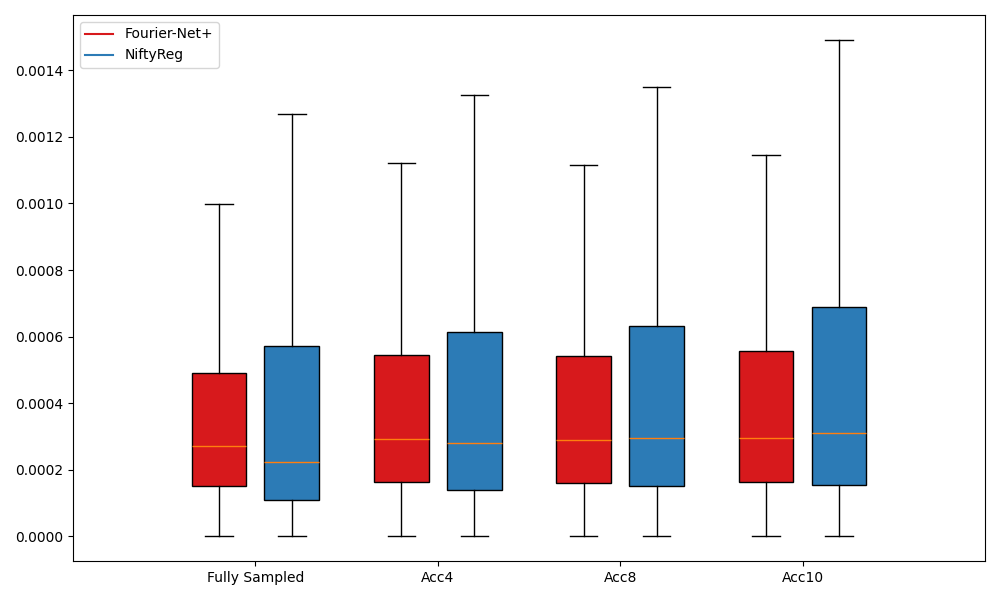
\includegraphics[width=.85\linewidth]{TestBenchmark_MSE_Boxplots.png} 
%	\caption{MSE results of \emph{Fourier-Net+} and \emph{NiftyReg} on the test set for fully sampled and subsampled (Acc4, Acc8, Acc10) data.}
%	\label{fig:TestBenchmark_MSE_Boxplots}
%\end{figure}
%
%\begin{figure}[htpb]
%	\centering
%	\graphicspath{{images/}{\main/images/}}
%	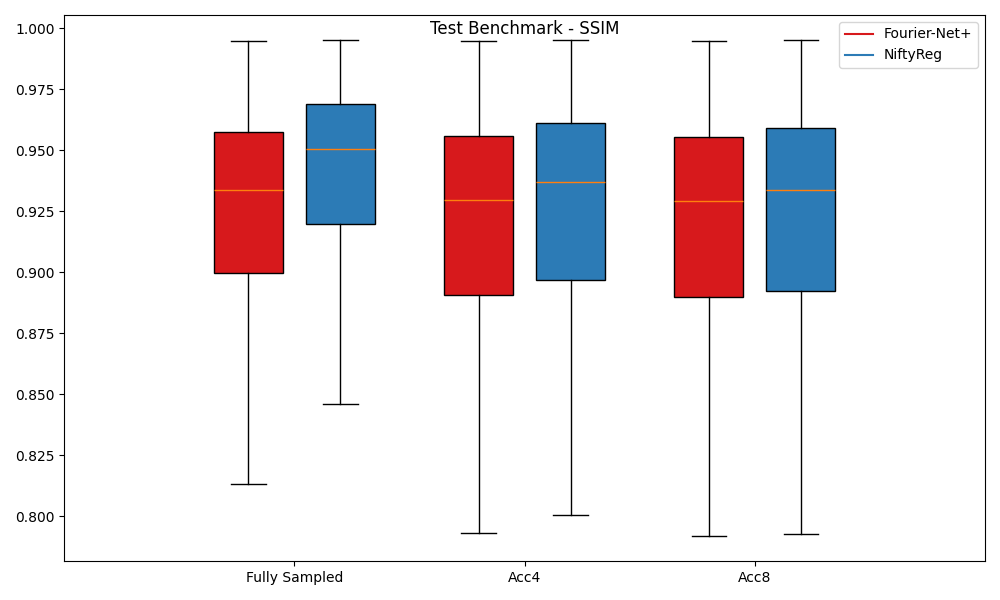
\includegraphics[width=.85\linewidth]{TestBenchmark_SSIM_Boxplots.png} 
%	\caption{SSIM results of \emph{Fourier-Net+} and \emph{NiftyReg} on the test set for fully sampled and subsampled (Acc4, Acc8, Acc10) data.}
%	\label{fig:TestBenchmark_SSIM_Boxplots}
%\end{figure}

\begin{figure}[h] %tpb
	\centering
	\graphicspath{{images/}{\main/images/}}
	\begin{subfigure}{0.495\textwidth}
    		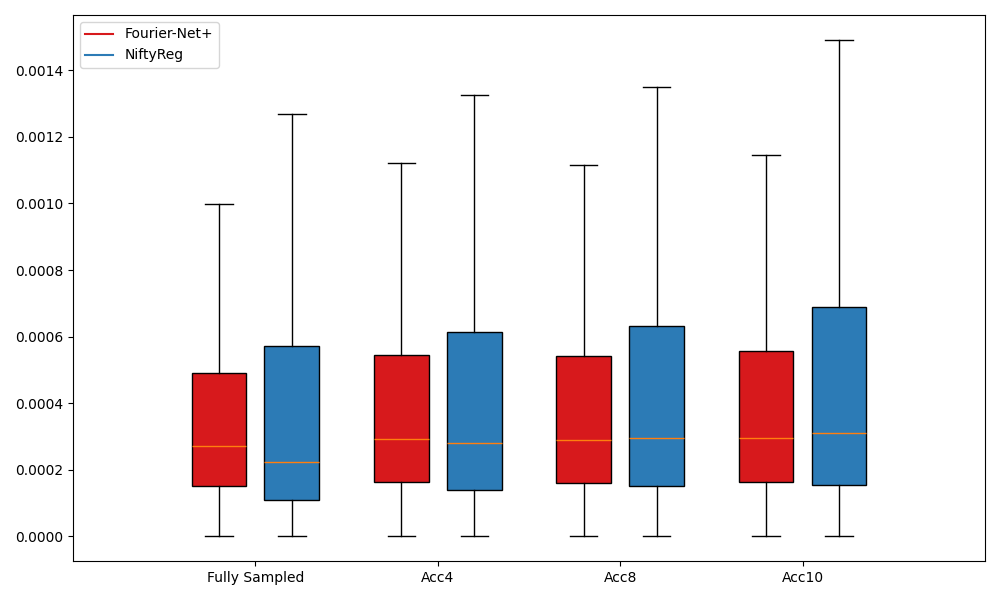
\includegraphics[width=\textwidth]{TestBenchmark_MSE_Boxplots.png}
    		\caption{Boxplot of MSE results.}
    		\label{fig:TestBenchmark_MSE_Boxplots}
	\end{subfigure}
	\hfill
	\begin{subfigure}{0.495\textwidth}
    		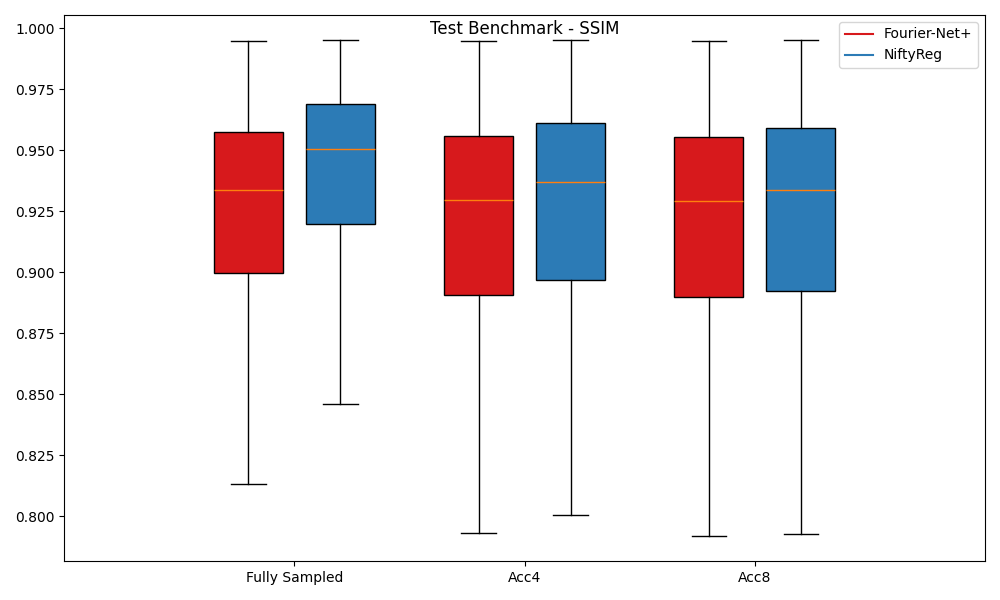
\includegraphics[width=\textwidth]{TestBenchmark_SSIM_Boxplots.png}
    		\caption{Boxplot of SSIM results.}
    		\label{fig:TestBenchmark_SSIM_Boxplots}
	\end{subfigure}
	\caption{Boxplots for MSE and SSIM results of the test set for fully sampled and subsampled (Acc4, Acc8, Acc10) data for both \emph{Fourier-Net+} and \emph{NiftyReg}.}
	\label{fig:TestBenchmark_Boxplots}
\end{figure}

\section{Further Tests on the ACDC Dataset}
Due to the limitations of the \emph{CMRxRecon} dataset in terms of segmentations, the registration performance is further evaluated on the \emph{ACDC} dataset. Some of the parameter studies done on \emph{CMRxRecon} were repeated, others were added to further test the networks ability.

\subsection{Fourier-Net versus Fourier-Net+} \label{SubSec:ResultsFourier-NetvsFourier-Net+ACDC}
Again, \emph{Fourier-Net}, \emph{Fourier-Net+} and \emph{4xFourier-Net} are compared in terms of registration performance and inference time (on GPU) together with their diffeomorphic versions, however, versions with dense instead of band-limited displacements are also added as a baseline for peak performance as these utilize all of the k-space information. The memory consumption is also added to the comparison with the number of parameters, mult-add operations and the total memory. The latter is only given for the dense and normal versions as the diffeomorphic version required roughly the same amount of memory as the normal ones, while the dense versions have a slightly larger encoder. 
%All \emph{Fourier-Net+} and \emph{4xFourier-Net} variants use a FT crop size of $48 \times 48$. All networks used MSE-loss etc.
Note that all network variants were trained for 6 epochs. The results can be seen in Table~\ref{tab:Fourier-NetvsFourier-Net+ACDC}.\\
For the dense displacement variants the diffeomorphic transform increases the performance in terms of Dice score (with and without the background label) slightly for \emph{Fourier-Net} and \emph{4xFourier-Net}, but decreases for \emph{Fourier-Net+}. The SSIM decreases for all models slightly, while the MSE stays about the same. Unsurprisingly, the percentage of non-positive Jabobian determinants goes down for the diffeomorphic variants. The times between the baseline and diffeomorphic versions do not vary a lot with the \emph{Fourier-Net} being faster without the diffeomorphis, while \emph{Fourier-Net+} and \emph{4xFourier-Net} are faster. \\
The results for the band-limited versions are very similar with \emph{Fourier-Net} and \emph{Fourier-Net+} performing slightly worse in terms of Dice (with background) with the diffeomorphis, while \emph{4xFourier-Net} performs better by almost 2$\%$. When excluding the background label \emph{Fourier-Net} again performs slightly worse, but \emph{Fourier-Net+} and \emph{4xFourier-Net} both improve, the latter with almost 3$\%$ more than the baseline version. These changes are not consistent with the dense displacement versions, however, the band-limited \emph{4xFourier-Net} version might be an outlier, as all of the other models are not affected as much by the diffeomorphic transform. The SSIM values slightly decrease for \emph{Fourier-Net} and \emph{Fourier-Net+} with the diffeomorphism, but again improve slightly for \emph{4xFourier-Net}. The MSE is slightly better for \emph{Fourier-Net} and \emph{4xFourier-Net}, but a bit worse for \emph{Fourier-Net+}. The percentage of non-positive Jabobian determinants again decreases for the diffeomorphic variants, which is consistent with the previous observations on the dense displacement versions. The times again vary slightly with \emph{Fourier-Net} and \emph{Fourier-Net+} being a bit slower, while \emph{4xFourier-Net} is quite a bit faster.\\
Now to the difference between the dense and band-limited displacement. Overall, the dense displacement versions perform better in terms of Dice score for all models both with and without the background label. This is to be expected as the dense displacement versions can use all of the available k-space data for the registration task, while the band-limited versions have only a limited amount of k-space data, directly impacting and limiting their performance. The dense displacement is also better in the SSIM metric, however the difference is not quite as large as with the Dice scores. As the differences between the frames is not quite as large, the weaker registration performance does not impact this metric as much as the Dice score, which is focused on the moving cardiac region. The same is true for the MSE, but the dense displacement is again far superior. Only in terms of the percentage of non-positive Jabobian determinants does the band-limited displacement actually perform better as the band-limiting probably allows for only a smaller deformation. However, the difference is still very small, especially for the diffeomorhpic versions, and it could be argued that a better registration performance at the cost of some image folding is an acceptable trade-off. In terms of inference time the dense displacement variants are surprisingly slightly faster despite having a larger encoder, however all of the model are in the low milliseconds ($<40~ms$). Last but not least, the memory consumption needs to be addressed. The dense displacment variants have a larger encoder as discussed before and thus have a lot more parameters, especially for the more optimized \emph{Fourier-Net+} and \emph{4xFourier-Net} (about 5 times more). The number of Mult-Adds and the amount of total memory are more than doubled (almost tripled for \emph{4xFourier-Net}) for the dense displacement versions compared to those with a band-limited displacement across all models.

\begin{table}[H] %htpb
	%\scriptsize
	\centering
	\caption{Results for \emph{Fourier-Net}, \emph{Fourier-Net+} and \emph{4xFourier-Net+} with both dense and band-limited displacement fields as well as diffeomorphic transforms on the fully sampled \emph{ACDC} test data.}
	\label{tab:Fourier-NetvsFourier-Net+ACDC}
	\begin{tabular}{c c c c} %
		\toprule
		\multirow{2}{*}{Metrics} & \multicolumn{3}{c}{Dense Displacement} \\
		\cline{2-4} 
		 & Fourier-Net & Fourier-Net+ & 4xFourier-Net+\\	
		\midrule
		$\%$ Dice & $78.22 \pm 13.84$ & $78.43 \pm 13.96$ & $79.34 \pm 14.03$\\
		$\%$ Dice* & $71.03 \pm 18.87$ & $70.50 \pm 19.17$ & $72.02 \pm 18.94$ \\
		$\%$ SSIM & $91.92 \pm 3.32$ & $89.09 \pm 4.10$ & $89.65 \pm 3.85$\\
		MSE (m) & $0.09 \pm 0.06$ & $0.17 \pm 0.13$ & $0.15 \pm 0.12$ \\
		$\% \, |J_{\phi}|\leq0$ & $0.53 \pm 0.52$ & $0.32 \pm 0.55$ & $0.04 \pm 0.09$ \\
		Time [s] 	  & 0.0070 	& 0.0107 	& 0.0219 \\
		\midrule
		 & Diff-Fourier-Net & Diff-Fourier-Net+ & Diff-4xFourier-Net+\\		
		\midrule
		$\%$ Dice & $78.56 \pm 14.13$ & $77.88 \pm 13.81$ & $79.49 \pm 14.26$\\
		$\%$ Dice* & $71.31 \pm 19.13$ & $70.19 \pm 18.82$ & $72.12 \pm 19.33$ \\
		$\%$ SSIM & $91.79 \pm 3.38$ & $89.08 \pm 4.10$ & $89.62 \pm 3.98$\\
		MSE (m) & $0.09 \pm 0.06$ & $0.16 \pm 0.13$ & $0.15 \pm 0.12$ \\
		$\% \, |J_{\phi}|\leq0$ & $0.03 \pm 0.06$ & $0.00 \pm 0.00$ & $0.00 \pm 0.00$ \\
		Time [s] 	  & 0.0082  & 0.0075 & 0.0203 \\
		\midrule
		Parameters    & 645,216 	& 380,470 	& 1,521,880 \\
		Mult-Adds (G) & 1.12  	& 0.04  		& 0.18 \\
		Memory [MB]   & 97.63   	& 5.81   	& 21.90 \\
		\midrule
		\multirow{2}{*}{Metrics} & \multicolumn{3}{c}{Band-limited Displacement} \\
		\cline{2-4} 
		 & Fourier-Net & Fourier-Net+ & 4xFourier-Net+\\		
		\midrule
		$\%$ Dice & $77.95 \pm 14.71$ & $75.35 \pm 14.28$ & $76.59 \pm 14.84$\\
		$\%$ Dice* & $69.96 \pm 21.55$ & $64.74 \pm 21.12$ & $66.82 \pm 21.55$ \\
		$\%$ SSIM & $91.35 \pm 3.51$ & $88.42 \pm 3.94$ & $88.59 \pm 4.23$\\
		MSE (m) & $1.00 \pm 0.71$ & $2.06 \pm 1.54$ & $1.92 \pm 1.46$ \\
		$\% \, |J_{\phi}|\leq0$ & $0.36 \pm 0.38$ & $0.13 \pm 0.35$ & $0.03 \pm 0.12$ \\
		Time [s] & 0.0145 & 0.0145 & 0.0335 \\
		\midrule
		 & Diff-Fourier-Net & Diff-Fourier-Net+ & Diff-4xFourier-Net+\\		
		\midrule
		$\%$ Dice & $77.93 \pm 14.93$ & $75.17 \pm 13.43$ & $78.20 \pm 14.01$\\
		$\%$ Dice* & $69.91 \pm 21.99$ & $65.67 \pm 18.61$ & $69.61 \pm 19.11$ \\
		$\%$ SSIM & $91.24 \pm 3.56$ & $87.81 \pm 3.94$ & $88.81 \pm 4.13$\\
		MSE (m) & $0.98 \pm 0.67$ & $2.29 \pm 1.61$ & $1.85 \pm 1.41$ \\
		$\% \, |J_{\phi}|\leq0$ & $0.01 \pm 0.03$ & $0.00 \pm 0.00$ & $0.00 \pm 0.00$ \\
		Time [s] 	  & 0.0150  & 0.0207 & 0.0188 \\
		\midrule
		Parameters    & 434,519 & 75,429 & 301,716 \\
		Mult-Adds (M) & 595.04  & 10.98  & 43.91 \\
		Memory [MB]   & 44.69   & 2.25   & 7.66 \\
		\bottomrule
	\end{tabular}	
\end{table}


\subsection{Starting Channel Size} \label{SubSec:ResultsStartingChannelsACDC}
Next, the impact of the starting channels was examined. For this, \emph{Fourier-Net+} and \emph{4xFourier-Net+} were trained with four different channel sizes: $8$, $16$, $32$ and $64$. The memory consumption as well as inference time on the GPU were calculated to extend the evaluation given by the other metrics. All network variants were trained for 6~epochs. The results can be seen in Table~\ref{tab:StartingChannelsFourierNet+ACDC}.\\
For both \emph{Fourier-Net+} and \emph{4xFourier-Net+} there is a clear increase in Dice (with and without the background label) with larger channel sizes as more features increase the registration performance. The SSIM and MSE metrics only increase marginally with larger channel size. The percentage of non-positive Jabobian determinants actually decreases as the registration performance increases, likely due to better/more features enabling a smoother and better displacement field to be generated by the models. \\
The inference time is not heavily impacted by channel size as the times remain very similar for all sizes. The memory however increases exponentially when doubling the channel sizes as all layers are effected, not just the starting one as the name suggests. Thus the number of parameters drastically increases with starting size leading to an increase in Mult-Add and thus overall memory. As \emph{4xFourier-Net+} is just a cascaded version of \emph{Fourier-Net+} a channel size of 16 for the latter is about the same as channel size~8 for the cascaded version and so on. Thus it seems that there is no point at which both the performance and memory consumption are maximized at the same time. This can also be seen in the direct comparison between \emph{Fourier-Net+} and \emph{4xFourier-Net+}, where the latter has a better performance, but also needs more memory. While an increase of channel size also increases performance in terms of Dice (with the background label) by $0.36\%$, $0.43\%$ and $0.41\%$ for the latter, which is quite consistent, it can be observed that an increase of channel size for \emph{Fourier-Net+} has an bigger impact at the beginning ($1.38\%$, $0.78\%$ and $0.15\%$) and fades towards larger channels sizes. This effect can also be seen when excluding the background label ($0.69\%$, $0.78\%$ and $0.42\%$ for \emph{4xFourier-Net+} compared to $2.16\%$, $1.09\%$ and $0.10\%$ for \emph{Fourier-Net+}), but is less pronounced for the SSIM and MSE as these do not capture the difference in the cardiac regions as well. Note that all versions of \emph{Fourier-Net+} and \emph{4xFourier-Net+} are smaller in terms of total memory than \emph{Fourier-Net} with channel size~8 (44.69 MB), except for \emph{4xFourier-Net+} with channel size~64.

\begin{table}[h] %tpb
	%\scriptsize
	\centering
	\caption{Results for different starting channel sizes of \emph{Fourier-Net+} and \emph{4xFourier-Net+} on the fully sampled \emph{ACDC} test data.}
	\label{tab:StartingChannelsFourierNet+ACDC}
	\begin{tabular}{c c c c c} %
		\toprule
		\multirow{2}{*}{Metrics} & \multicolumn{4}{c}{Starting Channels - Fourier-Net+} \\
		\cline{2-5}
		 & 8 & 16 & 32 & 64 \\		
		\midrule
		$\%$ Dice & $75.50 \pm 13.79$ & $76.88 \pm 13.86$ & $77.66 \pm 13.60$ & $77.81 \pm 13.76$ \\
		$\%$ Dice* & $65.70 \pm 18.96$ & $67.86 \pm 19.06$ & $68.95 \pm 18.65$ & $69.05 \pm 18.80$ \\
		$\%$ SSIM & $88.05 \pm 3.89$ & $88.67 \pm 3.88$ & $88.83 \pm 3.83$ & $89.02 \pm 3.67$ \\
		MSE (m) & $0.22 \pm 0.16$ & $0.20 \pm 0.15$ & $0.19 \pm 0.15$ & $0.19 \pm 0.15$ \\
		$\% \, |J_{\phi}|\leq0$ & $0.07 \pm 0.25$ & $0.04 \pm 0.14$ & $0.01 \pm 0.04$ & $0.00 \pm 0.03$ \\
		Time [s] 	  & 0.0072 & 0.0072 & 0.0080 & 0.0079 \\
		Parameters 	  & 75,429 	& 300,477 	& 1,199,469 	& 4,793,037 \\
		Mult-Adds (M) & 10.98 	& 42.89 		& 169.54 	& 674.10 \\
		Memory [MB] 	  & 2.25 	& 4.64 		& 11.22 		& 31.57 \\
		\midrule		
		\multirow{2}{*}{Metrics} & \multicolumn{4}{c}{Starting Channels - 4xFourier-Net+} \\
		\cline{2-5} 
		 & 8 & 16 & 32 & 64 \\		
		\midrule
		$\%$ Dice & $77.54 \pm 13.73$ & $77.90 \pm 13.92$ & $78.33 \pm 14.14$ & $78.74 \pm 13.91$ \\
		$\%$ Dice* & $68.52 \pm 18.62$ & $69.21 \pm 19.02$ & $69.99 \pm 19.21$ & $70.41 \pm 19.02$ \\
		$\%$ SSIM & $88.70 \pm 4.17$ & $88.89 \pm 4.05$ & $89.08 \pm 4.01$ & $89.29 \pm 3.74$ \\
		MSE (m) & $0.19 \pm 0.14$ & $0.19 \pm 0.14$ & $0.18 \pm 0.14$ & $0.18 \pm 0.14$ \\
		$\% \, |J_{\phi}|\leq0$ & $0.02 \pm 0.07$ & $0.01 \pm 0.04$ & $0.01 \pm 0.05$ & $0.00 \pm 0.00$ \\
		Time [s] 	  & 0.0301 	& 0.0244 	& 0.0297 	& 0.0277 \\
		Parameters 	  & 301,716 	& 1,201,908 	& 4,797,876 	& 19,172,148 \\
		Mult-Adds (G) & 0.04 	& 0.17 		& 0.68 		& 2.70 \\
		Memory [MB] 	  & 7.66 	& 17.23 		& 43.56 		& 124.94 \\
		\bottomrule
	\end{tabular}	
\end{table}


\subsection{Fourier-Transform Crop Size} \label{SubSec:ResultsFTCropSize}
As a parameter specific to \emph{Fourier-Net+} and \emph{4xFourier-Net+}, the impact of the FT crop size used for compressing the images was analyzed. Four different sizes of the FT crop were used for training: $80 \times 168$, $40 \times 84$, $48 \times 48$ and $24 \times 24$. The experiments were again only conducted on the fully sampled data and each network trained for 5 epochs. The results can be seen in Table~\ref{tab:FTCropSize}. \\
The registration performance, as measured by the Dice score both with and without the background label, decreases drastically with a smaller crop size. This is as expected as the smaller FT drop compresses the images more thus making an accurate registration harder. The SSIM and MSE also get worse (SSIM decreases, MSE increases), however the amount of performance lost is hard to gauge, especially for the MSE metric. Interestingly, the percentage of non-positive Jabobian determinants actually decreases for smaller crop sizes, perhaps because the displacements on the compressed images are not as extreme and thus more smooth. Note however, that the crop size of $48 \times 48$ is a bit of an outlier in this regard breaking the trend with a higher percentage as $40 \times 84$. The time also seems to decrease slightly with a smaller crop, although this is quite noisy as the time from $80 \times 168$ to $40 \times 84$ is halved for \emph{Fourier-Net+}, but the time needed for $48 \times 48$ and $24 \times 24$ increases again very slightly. For \emph{4xFourier-Net+} the time decrease for all smaller crop sizes, except for $24 \times 24$.\\
The number of parameters does not change for different crop sizes as the networks themselves do not change, however the number of Mult-Adds and the total memory still change with the image size. Both decrease with a larger crop size as the image gets smaller. This effect is again not linear as a reduction in image size yields a larger reduction in memory going from $80 \times 168$ to $40 \times 84$ than from $48 \times 48$ to $24 \times 24$. Again, there is no sweet-spot to be found that maximizes both memory efficiency and registration performance similar to the experiments in the previous chapter.

\begin{table}[h] %tpb
	%\scriptsize
	\centering
	\caption{Results for four different FT crop sizes for \emph{Fourier-Net+} and \emph{4xFourier-Net+} examined on the fully sampled \emph{ACDC} test data.}
	\label{tab:FTCropSize}
	\begin{tabular}{c c c c c} %
		\toprule
		\multirow{2}{*}{Metrics} & \multicolumn{4}{c}{FT crop size - Fourier-Net+} \\
		\cline{2-5}
		 & $80 \times 168$ & $40 \times 84$ & $48 \times 48$ & $24 \times 24$ \\		
		\midrule
		$\%$ Dice & $78.24 \pm 14.43$ & $76.61 \pm 13.90$ & $75.27 \pm 13.49$ & $73.77 \pm 14.42$ \\
		$\%$ Dice* & $70.66 \pm 19.70$ & $67.60 \pm 19.24$ & $65.48 \pm 18.76$ & $63.37 \pm 20.07$ \\
		$\%$ SSIM & $89.81 \pm 4.09$ & $88.58 \pm 3.87$ & $87.98 \pm 3.91$ & $87.00 \pm 3.99$ \\
		MSE (m) & $0.15 \pm 0.12$ & $0.20 \pm 0.15$ & $0.22 \pm 0.16$ & $0.27 \pm 0.19$ \\
		$\% \, |J_{\phi}|\leq0$ & $0.22 \pm 0.46$ & $0.05 \pm 0.15$ & $0.09 \pm 0.25$ & $0.00 \pm 0.02$ \\		
		Time [s] 	  & 0.0158 & 0.0077 & 0.0079 & 0.0081 \\
		Parameters 	  & 75,429 & 75,429 & 75,429 & 75,429 \\
		Mult-Adds (M) & 64.03  & 16.37  & 10.98  & 2.74 \\
		Memory [MB] 	  & 9.51   & 2.97   & 2.25   & 1.12 \\
		\midrule
		\multirow{2}{*}{Metrics} & \multicolumn{4}{c}{FT crop size - 4xFourier-Net+} \\
		\cline{2-5}
		 & $80 \times 168$ & $40 \times 84$ & $48 \times 48$ & $24 \times 24$ \\		
		\midrule
		$\%$ Dice & $78.12 \pm 15.01$ & $77.49 \pm 14.67$ & $74.95 \pm 14.15$ & $72.58 \pm 14.67$ \\
		$\%$ Dice* & $70.08 \pm 21.92$ & $68.03 \pm 21.57$ & $64.54 \pm 20.75$ & $61.19 \pm 21.63$ \\
		$\%$ SSIM & $89.91 \pm 4.01$ & $89.03 \pm 3.98$ & $87.98 \pm 3.94$ & $87.02 \pm 3.95$ \\
		MSE (m) & $1.45 \pm 1.11$ & $1.81 \pm 1.37$ & $2.22 \pm 1.61$ & $2.64 \pm 1.84$ \\
		$\% \, |J_{\phi}|\leq0$ & $0.12 \pm 0.23$ & $0.03 \pm 0.15$ & $0.06 \pm 0.23$ & $0.02 \pm 0.15$ \\	
		Time [s] 	 & 0.0390  & 0.0301  & 0.0277  & 0.0289 \\
		Parameters 	 & 301,716 & 301,716 & 301,716 & 301,716 \\
		Mult-Adds (M)& 256.14  & 65.50   & 43.91   & 10.98 \\
		Memory [MB] 	 & 36.70   & 10.54   & 7.66    & 3.15 \\
		\bottomrule
	\end{tabular}
\end{table}

\subsection{Comparison with VoxelMorph} \label{SubSec:ResultsComparisonVoxelMorph}
In this test \emph{Fourier-Net}, \emph{Fourier-Net+} and \emph{4xFourier-Net+} are compared to the famous \emph{VoxelMorph}~\cite{Voxelmorph}. This unsupervised network brought deep learning based registration approaches into the mainstream and computes a dense displacement field in contrast to the band-limited displacement of the other networks. From the previous experiments a FT crop size of $48 \times 48$ and channel size of 16 was chosen to strike a good balance between performance and memory efficiency. The experiment was only done on the fully sampled test data and all networks were trained for 6 epochs. The results can be seen in Table~\ref{tab:CompareVoxelMorph}.\\
\emph{VoxelMorph} performs worst in terms of Dice score with the background label, however it does outperform \emph{Fourier-Net+} in Dice without the background label. The best registration performance in terms of Dice (both with and without the background label) has \emph{Fourier-Net} followed by \emph{4xFourier-Net+} as expected. \emph{VoxelMorph}, however, does perform best in terms of SSIM and MSE followed by \emph{Fourier-Net}, so it seems that the dense network aligns the overall image well, but struggles to compensate the strong changes in the cardiac region between frames. It is conspicuous, however, that the percentage of non-positive Jabobian determinants for \emph{VoxelMorph} is quite high with almost $90\%$ while the other models are all under one percent. This is perhaps caused by the dense displacement which causes a better overall alignment (as indicated by the good SSIM and MSE values) at the cost of more folding occurring. In terms of time \emph{4xFourier-Net+} is slowest followed by  \emph{VoxelMorph}, \emph{Fourier-Net} and \emph{Fourier-Net+}, however all pretty fast ($<30ms$). The model with the least amount of parameters and Mult-Adds is \emph{VoxelMorph}, however perhaps due to the dense displacment it needs quite a lot of memory with almost 40~MB. \emph{Fourier-Net} is the largest model in terms of model paramters, Mult-Adds and total memory (90~MB). \emph{Fourier-Net+} and \emph{4xFourier-Net+} both have a higher number of paramters and Mult-Adds, but a lower total amount of memory needed. Overall, \emph{4xFourier-Net+} is the only model that is truly more efficient and has better performance in terms of Dice than \emph{VoxelMorph}, as \emph{Fourier-Net+} is more efficient, but not necessarily better in terms of Dice score, while \emph{Fourier-Net} is far superior in registration performance (as measured by the Dice score), but also less efficient in terms of memory consumption.

\begin{table}[h] %tpb
	%\scriptsize
	\centering
	\caption{Comparison of \emph{Fourier-Net}, \emph{Fourier-Net+}, \emph{4xFourier-Net+} and \emph{VoxelMorph} with similarity metrics and memory consumption on the fully sampled \emph{ACDC} test data.}
	\label{tab:CompareVoxelMorph}
	\begin{tabular}{c c c c c} %
		\toprule
		 & Fourier-Net & Fourier-Net+ & 4xFourier-Net+ & VoxelMorph \\		
		\midrule
		$\%$ Dice & $78.31 \pm 13.96$ & $76.88 \pm 13.86$ & $77.90 \pm 13.92$ & $75.84 \pm 13.46$ \\
		$\%$ Dice* & $71.17 \pm 18.99$ & $67.86 \pm 19.06$ & $69.21 \pm 19.02$ & $68.25 \pm 18.36$ \\
		$\%$ SSIM & $91.53 \pm 3.49$ & $88.67 \pm 3.88$ & $88.89 \pm 4.05$ & $93.53 \pm 3.30$ \\
		MSE (m) & $0.09 \pm 0.07$ & $0.20 \pm 0.15$ & $0.19 \pm 0.14$ & $0.06 \pm 0.04$ \\
		$\% \, |J_{\phi}|\leq0$ & $0.44 \pm 0.45$ & $0.04 \pm 0.14$ & $0.01 \pm 0.04$ & $89.96 \pm 1.32$ \\
		Time [s] 	  & 0.0099    & 0.0071 	& 0.0244  	& 0.0145 \\
		Parameters 	  & 1,735,447 & 300,477 	& 1,201,908 	& 84,322 \\
		Mult-Adds (G) & 2.35      & 0.04289  & 0.17157  	& 0.00157 \\
		Memory [MB] 	  & 90.08     & 4.64   	& 17.23    	& 39.04 \\
		\bottomrule
	\end{tabular}		
\end{table}


\subsection{Dense Displacement on Accelerated Data} \label{SubSec:DenseDisplacementAcc}
The difference between a dense displacement field and a band-limited one was already explored in section~\ref{SubSec:ResultsFourier-NetvsFourier-Net+ACDC}. However, the results in Table~\ref{tab:Fourier-NetvsFourier-Net+ACDC} only include fully sampled data, not accelerated data. These new tests again included \emph{Fourier-Net}, \emph{Fourier-Net+} and \emph{4xFourier-Net+}, but are extended to subsampled data. Results for Acc4 data can be seen in Table~\ref{tab:DenseDisplacementAcc4}, for Acc8 data in Table~\ref{tab:DenseDisplacementAcc8} and for Acc10 in Table~\ref{tab:DenseDisplacementAcc10}. \\
For Acc4, the dense version of \emph{Fourier-Net} performed worse than the band-limited version in terms of Dice, as we expected, however this is not the case for \emph{Fourier-Net+} and \emph{4xFourier-Net+} where the performance decreases for the band-limited versions as indicated by the dice score. The same is true for the SSIM and MSE values. The percentage of non-positive Jabobian determinants is higher for the band-limited \emph{Fourier-Net}, while band-limited \emph{Fourier-Net+} and \emph{4xFourier-Net+} show no folding. While this at first seems like a positive metric it can also indicate a lack of complex displacements which could explain the lower performance. All band-limited versions are faster due to the smaller network size as the encoder lack some layers compared to the dense versions.\\
For Acc8 all band-limited networks perform worse in terms of Dice, SSIM and MSE. The percentage of non-positive Jabobian determinants is again higher for the band-limited \emph{Fourier-Net} compared to the dense version, while the band-limited \emph{Fourier-Net+} and \emph{4xFourier-Net+} show no folding. The band-limited versions surprisingly are slower compared to the dense versions except for \emph{Fourier-Net+}. \\
For Acc10, similar to Acc4, band-limited \emph{Fourier-Net} performs better in terms of Dice, SSIM and MSE, while band-limited \emph{Fourier-Net+} and \emph{4xFourier-Net+} are again worse compared to the dense versions. The percentage of non-positive Jabobian determinants for the band-limited \emph{Fourier-Net} is lower than for the dense version this time, while band-limited \emph{Fourier-Net+} and \emph{4xFourier-Net+} again show no folding. As for the Acc4 data, the band-limited networks are faster in terms of inference time.\\
The results for the accelerated data are not quite consistent as the band-limited \emph{Fourier-Net} performs better for Acc4 and Acc10, but not for Acc8. Band-limited \emph{Fourier-Net+} and \emph{4xFourier-Net+} perform consistently worse than their dense versions across all acceleration levels. The band-limiting of the displacement seems to help with avoiding folding and in most cases decrease inference time. Our hypothesis that the advantage of the dense displacement compared to the band-limited displacement disappears for accelerated data does not seem to hold except for \emph{Fourier-Net} on Acc4 and Acc10 data.


\begin{table}[h] %tpb
	%\scriptsize
	\centering
	\caption{Results for \emph{Fourier-Net}, \emph{Fourier-Net+} and \emph{4xFourier-Net+} with both dense and band-limited displacement fields on the Acc4 \emph{ACDC} test data.}
	\label{tab:DenseDisplacementAcc4}
	\begin{tabular}{c c c c} %
		\toprule
		\multirow{2}{*}{Metrics} & \multicolumn{3}{c}{Dense Displacement} \\
		\cline{2-4} 
		 & Fourier-Net & Fourier-Net+ & 4xFourier-Net+\\	
		\midrule
		$\%$ Dice & $77.37 \pm 13.92$ & $-$ & $-$\\
		$\%$ Dice* & $68.98 \pm 19.10$ & $-$ & $-$ \\
		$\%$ SSIM & $84.75 \pm 7.01$ & $-$ & $-$\\
		MSE (m) & $0.08 \pm 0.05$ & $-$ & $-$ \\
		$\% \, |J_{\phi}|\leq0$ & $0.16 \pm 0.19$ & $-$ & $-$ \\
		Time [s] 	  & 0.0085 & - & -  \\
		\midrule
		\multirow{2}{*}{Metrics} & \multicolumn{3}{c}{Band-limited Displacement} \\
		\cline{2-4} 
		 & Fourier-Net & Fourier-Net+ & 4xFourier-Net+\\		
		\midrule
		$\%$ Dice & $76.55 \pm 13.89$ & $76.20 \pm 13.57$ & $77.23 \pm 13.73$\\
		$\%$ Dice* & $67.90 \pm 19.44$ & $66.30 \pm 19.01$ & $67.67 \pm 18.97$ \\
		$\%$ SSIM & $82.93 \pm 8.12$ & $77.74 \pm 10.69$ & $77.96 \pm 10.57$\\
		MSE (m) & $0.10 \pm 0.06$ & $0.19 \pm 0.14$ & $0.18 \pm 0.13$ \\
		$\% \, |J_{\phi}|\leq0$ & $0.35 \pm 0.41$ & $0.01 \pm 0.05$ & $0.00 \pm 0.02$ \\
		Time [s] 	  & 0.0069  	& 0.0065 	& 0.0312  \\
		\bottomrule
	\end{tabular}	
\end{table}


\begin{table}[H] %tpb
	%\scriptsize
	\centering
	\caption{Results for \emph{Fourier-Net}, \emph{Fourier-Net+} and \emph{4xFourier-Net+} with both dense and band-limited displacement fields on the Acc8 \emph{ACDC} test data.}
	\label{tab:DenseDisplacementAcc8}
	\begin{tabular}{c c c c} %
		\toprule
		\multirow{2}{*}{Metrics} & \multicolumn{3}{c}{Dense Displacement} \\
		\cline{2-4} 
		 & Fourier-Net & Fourier-Net+ & 4xFourier-Net+\\	
		\midrule
		$\%$ Dice & $-$ & $-$ & $-$\\
		$\%$ Dice* & $-$ & $-$ & $-$ \\
		$\%$ SSIM & $-$ & $-$ & $-$\\
		MSE (m) & $-$ & $-$ & $-$ \\
		$\% \, |J_{\phi}|\leq0$ & $-$ & $-$ & $-$ \\
		Time [s] 	  & - & - & -  \\
		\midrule
		\multirow{2}{*}{Metrics} & \multicolumn{3}{c}{Band-limited Displacement} \\
		\cline{2-4} 
		 & Fourier-Net & Fourier-Net+ & 4xFourier-Net+\\		
		\midrule
		$\%$ Dice & $75.52 \pm 13.69$ & $75.76 \pm 13.43$ & $76.56 \pm 13.47$\\
		$\%$ Dice* & $66.86 \pm 18.97$ & $65.45 \pm 18.63$ & $66.81 \pm 18.77$ \\
		$\%$ SSIM & $89.51 \pm 3.34$ & $86.30 \pm 4.18$ & $86.29 \pm 4.23$\\
		MSE (m) & $0.06 \pm 0.04$ & $0.13 \pm 0.11$ & $0.13 \pm 0.11$ \\
		$\% \, |J_{\phi}|\leq0$ & $0.27 \pm 0.29$ & $0.03 \pm 0.11$ & $0.00 \pm 0.02$ \\
		Time [s] 	  & 0.0090 & 0.0077 & 0.0466  \\
		\bottomrule
	\end{tabular}	
\end{table}


\begin{table}[H] %tpb
	%\scriptsize
	\centering
	\caption{Results for \emph{Fourier-Net}, \emph{Fourier-Net+} and \emph{4xFourier-Net+} with both dense and band-limited displacement fields on the Acc10 \emph{ACDC} test data.}
	\label{tab:DenseDisplacementAcc10}
	\begin{tabular}{c c c c} %
		\toprule
		\multirow{2}{*}{Metrics} & \multicolumn{3}{c}{Dense Displacement} \\
		\cline{2-4} 
		 & Fourier-Net & Fourier-Net+ & 4xFourier-Net+\\	
		\midrule
		$\%$ Dice & $-$ & $-$ & $-$\\
		$\%$ Dice* & $-$ & $-$ & $-$ \\
		$\%$ SSIM & $-$ & $-$ & $-$\\
		MSE (m) & $-$ & $-$ & $-$ \\
		$\% \, |J_{\phi}|\leq0$ & $-$ & $-$ & $-$ \\
		Time [s] 	  & - & - & -  \\
		\midrule
		\multirow{2}{*}{Metrics} & \multicolumn{3}{c}{Band-limited Displacement} \\
		\cline{2-4} 
		 & Fourier-Net & Fourier-Net+ & 4xFourier-Net+\\		
		\midrule
		$\%$ Dice & $76.87 \pm 13.97$ & $76.10 \pm 13.83$ & $76.98 \pm 13.57$\\
		$\%$ Dice* & $68.24 \pm 19.27$ & $66.27 \pm 19.20$ & $67.40 \pm 18.90$ \\
		$\%$ SSIM & $92.77 \pm 2.74$ & $90.32 \pm 3.29$ & $90.42 \pm 3.33$\\
		MSE (m) & $0.05 \pm 0.04$ & $0.12 \pm 0.12$ & $0.11 \pm 0.11$ \\
		$\% \, |J_{\phi}|\leq0$ & $0.11 \pm 0.15$ & $0.01 \pm 0.05$ & $0.00 \pm 0.03$ \\
		Time [s] 	  & 0.0081 & 0.0096 & 0.0279  \\
		\bottomrule
	\end{tabular}	
\end{table}
 
\newpage
\subsection{Comparison on Subsampled Data} \label{SubSec:ResultsComparisonSubsampling}
In section~\ref{SubSec:ComparisonVoxelMorph}, \emph{Fourier-Net}, \emph{Fourier-Net+} and \emph{4xFourier-Net+} were already compared to \emph{VoxelMorph}, however, these comparisons were only done on fully sampled, not accelerated data. To further add to the comparison, \emph{NiftyReg} was again used as a traditional registration algorithm. The unaligned test image pairs were treated as a baseline for the lower bound of registration performance. The results can be seen in Table~\ref{tab:ComparisonSubsamplingACDC} for fully sampled ($R=0$), Acc4 ($R=4$), Acc8 ($R=8$) and Acc10 ($R=10$) \emph{ACDC} test data. Values which are worse than the baseline are marked in red, while the best results for each acceleration level and metric is highlighted with blue. All times are computed on CPU due to \emph{NiftyReg} only working on the CPU as the GPU capable versions were deprecated. Additionally, Figure~\ref{fig:Boxplots_DiceScores} shows the performance of the methods for each segmentation label (excluding the background) while Figure~\ref{fig:TestExamples} shows example images and segmentations warped by the different methods for a visual comparison.\\
For $R=0$, \emph{Fourier-Net} performs best in terms of Dice (both with and without the background label), closely followed by \emph{4xFourier-Net+} while \emph{NiftyReg} performs worse than the baseline. \emph{VoxelMorph} performs best in terms of SSIM, followed by \emph{Fourier-Net} and \emph{NiftyReg}, as well as MSE where \emph{NiftyReg} again performs worse than the baseline on the fully sampled data. \emph{NiftyReg} and \emph{4xFourier-Net+} had the lowest percentage of non-positive Jabobian determinants while \emph{VoxelMorph} had the highest value by far (almost $50\%$ while the other method were all under $1\%$) indicating folding. \emph{Fourier-Net} is the fastest method with under $0.1s$ per image pair, while \emph{NiftyReg} takes over $100s$ making it the slowest by a large margin (all other methods were under $1s$).\\
For $R=4$, the registration performance decreases for all methods with \emph{NiftyReg} again performing worse than the baseline, while \emph{4xFourier-Net+} performed best in terms of Dice with the background label, while \emph{Fourier-Net} performed best in Dice without the background. \emph{VoxelMorph} performs best in terms of SSIM and MSE, followed by \emph{Fourier-Net} and \emph{NiftyReg}, with none of methods performing worse than the baseline. \emph{4xFourier-Net+} again has the lowest percentage of non-positive Jabobian determinants closely followed by \emph{Fourier-Net+}, while \emph{VoxelMorph}, similar to the fully sampled data, has the highest value. In terms of time \emph{NiftyReg} is again the worst method with about $80s$, while all other methods need around $0.1s$ with \emph{Fourier-Net+} being the fastest.\\
For $R=8$, \emph{4xFourier-Net+} again performs best for Dice with the background label, while \emph{Fourier-Net} performs best in term of Dice without the background label. \emph{NiftyReg} performs worse than the baseline in terms of Dice (both with and without the background label). \emph{NiftyReg} again performs best for SSIM and MSE followed by \emph{Fourier-Net} and \emph{NiftyReg}. \emph{4xFourier-Net+} has the lowest percentage of non-positive Jabobian determinants followed by \emph{Fourier-Net+}, while \emph{VoxelMorph} again has the worst value. \emph{NiftyReg} is the worst method in terms of time with over $80s$, similar to $R=4$, while \emph{Fourier-Net+} again is the fastest, however, being slightly slower than before.\\
For $R=10$, \emph{4xFourier-Net+} performs best in terms of Dice with the background label, while \emph{Fourier-Net} performs best in terms of Dice without the background. \emph{NiftyReg} again performs worse than the baseline for Dice (both with and without background label). \emph{VoxelMorph} is again the best method in terms of SSIM and MSE, followed by \emph{Fourier-Net} and \emph{NiftyReg} with no method being worse than the baseline. \emph{4xFourier-Net+} has again the lowest percentage of non-positive Jabobian determinants closely followed by \emph{Fourier-Net+}, while \emph{VoxelMorph} has the worst value like before. \emph{Fourier-Net+} is again the fastest method with under $0.01s$, while \emph{NiftyReg} is again the slowest despite its best time yet with about $47s$.\\
To summarize, \emph{Fourier-Net+} is the fastest method for all acceleration levels while \emph{NiftyReg} is far behind all other methods in 
%terms of 
execution time as it is not machine learning based. \emph{VoxelMorph} performs best in terms of SSIM and MSE for all acceleration levels, however it also has the highest percentage of non-positive Jabobian determinants by a large margin indicating potential folding artifacts. \emph{4xFourier-Net+} performs best in terms of Dice with the background label except for $R=0$ while consistently having the lowest percentage of non-positive Jabobian determinants with a mean value under $0.005\%$ for all acceleration levels. \emph{Fourier-Net+} performs well in terms of Dice (with and without the background label), however it does not manage to surpass the other \emph{Fourier-Net} variants despite having the second lowest percentage of non-positive Jabobian determinants across the acceleration levels. \emph{Fourier-Net} performs best in terms of Dice without the background label for all acceleration level as well as in Dice with the background for $R=0$. \emph{NiftyReg} consistently performs worse than the baseline in terms of Dice (with and without the background) across all acceleration levels while having decent SSIM and MSE values. The performance, in general, decreased for all methods for higher acceleration levels as seen in the Dice metric, however, perhaps counter-intuitively, the SSIM is highest and the MSE the lowest for the $R=10$ baseline with only $R=4$ breaking the trend. This shows once again that image similarity metrics are not completely objective when it comes to evaluating registration performance across different acceleration levels.\\
To further evaluate the difference between the methods performance one can look at the Dice scores of the three individual cardiac labels. The results can be seen as boxplots in Figure~\ref{fig:Boxplot_DiceScores_LV-Cavity} for the left ventricle, Figure~\ref{fig:Boxplot_DiceScores_Myocardium} for the myocardium and Figure~\ref{fig:Boxplot_DiceScores_RV-Cavity} for the right ventricle.
%\\ As seen in Figure~\ref{fig:Boxplots_DiceScores}, 
The Dice scores for each label vary widely but the performance of all methods is best for the right ventricle and worst for the myocardium. This seems to be an underlying principle of the data as the same behavior can be seen in the unaligned baseline. \\
\emph{NiftyReg} performs well for the left ventricle, even surpassing \emph{VoxelMorph}, while it is the worst method for the myocardium (being only slightly better than the baseline) and the right ventricle (far worse than the baseline). Overall, \emph{NiftyReg} is not heavily affected by the artifacts present in the subsampled data, but is also not able to perform better than the other methods consistently. \\
\emph{VoxelMorph} performs best on the right ventricle compared to the other labels being close the \emph{Fourier-Net} variant for $R=0$, but falling off for the subsampled data, even performing worse than the baseline. It is better than the baseline, \emph{NiftyReg} and even \emph{Fourier-Net+} on $R=0$ for the myocardium, but again loses performance for the subsampled data. This trend also continues for the left ventricle were \emph{VoxelMorph} performs about as well as the baseline, but better than \emph{NiftyReg}, however ends up falling behind the baseline. Overall, \emph{VoxelMorph} is able to outperform the baseline, \emph{NiftyReg} and even \emph{Fourier-Net+} on one occasion, but is severely hampered by the artifacts caused by the subsampling of the k-space thus limiting its usability for accelerated MRI applications.\\
\emph{Fourier-Net} is consistently the best method for the challenging myocardium, however it is only about as good as \emph{Fourier-Net+} and \emph{4xFourier-Net+} for the left and right ventricle (even performing slightly worse than the baseline for $R=8$ on the latter). While \emph{Fourier-Net}, overall, is effected by the subsampling the effect is far less severe compared to \emph{VoxelMorph} and \emph{Fourier-Net} reaches a far better performance, especially for the challenging myocardium.\\
\emph{Fourier-Net+} performs well for the left ventricle being barely affected by the subsampling, although it is surpassed by \emph{Fourier-Net} on $R=0$ and by \emph{4xFourier-Net+} for $R=4$ and $R=10$. For the challenging myocardium \emph{Fourier-Net+} again performs well, but is surpassed by \emph{Fourier-Net} for all acceleration levels and only manages to beat \emph{4xFourier-Net+} for $R=10$. For the right ventricle \emph{Fourier-Net+} is among the best methods, even performing better than \emph{Fourier-Net} and \emph{4xFourier-Net+}  for $R=8$.\\
\emph{4xFourier-Net+} consistently has the best median value for the left ventricle and is close to being the best model for the right ventricle. Only on the myocardium it is consistently outperformed by \emph{Fourier-Net}.\\
In order to explain these differences one can look at the warped images and segmentations as well as the generated displacement fields visualized in Figure~\ref{fig:TestExamples}. For all acceleration levels, an example moving and fixed image can be compared to the warped images by the different methods. For further analysis, the corresponding segmentations (with Dice scores) and displacement fields for the methods are given.\\
For $R=0$, it is apparent that \emph{Fourier-Net+} and \emph{4xFourier-Net+} have very localized displacements centered on the cardiac region leading to a very smooth warped segmentation compared to \emph{Fourier-Net} and \emph{VoxelMorph} were the cardiac labels mix in some regions. Thus those networks have learned a less localized transformation, which can also be seen in the displacements. However, despite this \emph{Fourier-Net} still achieves the best Dice score with about $16\%$ increase compared to the baseline. While \emph{NiftyReg} does produce a very smooth warped segmentation the actual displacement is very small and not localized on the cardiac region leading to the worst Dice score of all methods.\\
For $R=4$, the image artifacts due to the subsampling are very apparent. The segmentations for the moving and fixed image obviously remain the same.
% despite the subsampling.
\emph{Fourier-Net+} and \emph{4xFourier-Net+} again have very smooth segmentations, however the displacements reflect the difficulties of adapting to subsampled data in becoming slightly less local. Surprisingly, \emph{NiftyReg} actually has a more localized displacement compared to the fully sampled data, however the segmentation looks less smooth and the Dice score is slightly lower. Somewhat similar, \emph{VoxelMorph} also has a more localized displacement leading to a smoother segmentation and a higher Dice score. The results of \emph{Fourier-Net} look overall very similar to the fully sampled case, perhaps with a bit more localized displacement leading to a smoother segmentation, although this does not lead to a better Dice Score.\\
For $R=8$, the displacements for all methods become more global due to the strong presence of image artifacts, however the Dice scores are better than before for all methods. \emph{NiftyReg} even outperforms \emph{VoxelMorph} for the first time. This trend does not continue for $R=10$, were \emph{NiftyReg} is again far behind all other methods in terms of Dice with a very much global displacement. \emph{VoxelMorph} seems to compensate more for the rippling artifacts present in the fixed image than for the change in the cardiac region as seen in the displacement. \emph{Fourier-Net}, \emph{Fourier-Net+} and \emph{4xFourier-Net+} do not share this behavior although their displacements also become more global and less focused on the cardiac region. The latter network performs best for the first time managing an increase in Dice of about $16\%$ compared to the baseline for this specific case despite the heavy subsampling showing the robustness of the network.

\begin{table}[h] %tpb
	%\tiny
	\scriptsize
	\centering
	\caption{Test results for \emph{NiftiReg} (NR), \emph{VoxelMorph} (VM), \emph{Fourier-Net} (F-Net), \emph{Fourier-Net+} (F-Net+) and \emph{4xFourier-Net+} (4xF-Net+) on the \emph{ACDC} test data from fully sampled (R=0) to Acc10 (R=10) with an unaligned baseline for comparison. The best results for each metric and subsampling are highlighted in blue, while values worse than the unaligned baseline are marked with red.}
	\label{tab:ComparisonSubsamplingACDC}
	\begin{tabular}{c c c c c c c c} 
		\toprule
		 & Method & $\%$ DICE & $\%$ DICE* & $\%$ SSIM & MSE (m) & $\% \, |J_{\phi}|\leq0$ & Time [s] \\
		% Fully Sampled (R=0)
		\midrule
		\multirow{6}{*}{\rotatebox{90}{R=0}} & Baseline & $70.85 \pm 18.27$  & $60.35 \pm 25.24$ & $86.39 \pm 4.08$ & $0.33 \pm 0.23$ & - & -\\  
		 & NR & \textcolor{red}{$70.74 \pm 13.77$} & \textcolor{red}{$57.56 \pm 18.86$} & $91.26 \pm 3.18$ & \textcolor{red}{$1.94 \pm 1.61$} & \textcolor{blue}{$0.00 \pm 0.02$} & 122.52\\
		 & VM & $75.84 \pm 13.46$ & $68.25 \pm 18.36$ & \textcolor{blue}{$93.53 \pm 3.30$} & \textcolor{blue}{$0.06 \pm 0.04$} & $49.98 \pm 0.73$ & 0.1845\\ 
		 %& LAPNet & $0.xxxx \pm 0.xxxx$ & $0.xxxx \pm 0.xxxx$  & $0.xxxxxx \pm 0.xxxxxx$ & $0.xxxxx \pm 0.xxxxx$  & -\\
		 & F-Net & \textcolor{blue}{$78.31 \pm 13.96$} & \textcolor{blue}{$71.17 \pm 18.99$} & $91.53 \pm 3.49$ & $0.09 \pm 0.07$ & $0.24 \pm 0.25$ & 0.1918\\ 
		 & F-Net+ & $76.88 \pm 13.86$ & $67.86 \pm 19.06$ & $88.67 \pm 3.88$ & $0.20 \pm 0.15$ & $0.02 \pm 0.08$ & \textcolor{blue}{0.0893} \\ 
		 & 4xF-Net+ & $77.90 \pm 13.92$ & $69.21 \pm 19.02$  & $88.89 \pm 4.05$ & $0.19 \pm 0.14$ & \textcolor{blue}{$0.00 \pm 0.02$} & 0.3262\\ 
		 	
		% 4x Accelerated (R=4) 				 		
		\midrule
		\multirow{6}{*}{\rotatebox{90}{R=4}} & Baseline & $70.85 \pm 18.27$ & $60.35 \pm 25.24$ & $76.80 \pm 11.02$ & $0.28 \pm 0.19$ & - & -\\  
		 & NR & \textcolor{red}{$69.89 \pm 13.73$} & \textcolor{red}{$56.47 \pm 17.86$} & $86.03 \pm 6.41$ & $0.15 \pm 0.14$ & $ 0.12 \pm 0.15$ & 80.08 \\  
		 & VM & $71.78 \pm 14.57$ & $63.15 \pm 18.98$ & \textcolor{blue}{$90.73 \pm 4.72$} & \textcolor{blue}{$0.04 \pm 0.03$} & $49.36 \pm 1.20$ & 0.1264\\  	
		 & F-Net & $76.55 \pm 13.89$ & \textcolor{blue}{$67.90 \pm 19.44$} & $82.93 \pm 8.12$ & $0.10 \pm 0.06$ & $0.19 \pm 0.23$ & 0.1006\\ 
		 & F-Net+ & $76.20 \pm 13.57$ & $66.30 \pm 19.01$ & $77.74 \pm 10.69$ & $0.19 \pm 0.14$ & $0.01 \pm 0.03$ & \textcolor{blue}{0.0294}\\ 
		 & 4xF-Net+ & \textcolor{blue}{$77.23 \pm 13.73$} & $67.67 \pm 18.97$ & $77.96 \pm 10.57$ & $0.18 \pm 0.13$ & \textcolor{blue}{$0.00 \pm 0.02$} & 0.1131\\ 
		  
%%%% Old Values %%%%		 
%		 & VoxelMorph & \textcolor{blue}{$73.45 \pm 13.40$} & \textcolor{blue}{$63.75 \pm 18.51$} & $78.56 \pm 7.32$ & \textcolor{blue}{$0.15 \pm 0.08$} & 0.1858\\  	
%		 & Fourier-Net & $72.30 \pm 14.04$ & $61.87 \pm 19.32$ & $78.77 \pm 7.22$ & $0.16 \pm 0.10$ & 0.1890\\ 
%		 & Fourier-Net+ & \textcolor{red}{$70.18 \pm 17.43$} & \textcolor{red}{$59.36 \pm 23.90$} & \textcolor{red}{$75.78 \pm 10.63$} & $0.28 \pm 0.19$ & \textcolor{blue}{0.0935}\\ 
%		 & 4xFourier-Net+ & \textcolor{red}{$70.36 \pm 16.63$} & \textcolor{red}{$59.47 \pm 22.80$} & \textcolor{red}{$75.91 \pm 10.72$} & $0.27 \pm 0.19$ & 0.3462\\  
		
		% 8x Accelerated (R=8) 
		\midrule
		\multirow{6}{*}{\rotatebox{90}{R=8}} & Baseline & $70.85 \pm 18.27$ & $60.35 \pm 25.24$ & $85.35 \pm 4.43$ & $0.22 \pm 0.17$ & - & -\\  
		 & NR & \textcolor{red}{$70.04 \pm 13.42$} & \textcolor{red}{$56.37 \pm 17.63$} & $91.07 \pm 2.80$ & $0.12 \pm 0.13$ & $0.08 \pm 0.10$ & 88.36 \\
		 & VM & $71.51 \pm 14.22$ & $62.17 \pm 18.80$ & \textcolor{blue}{$94.17 \pm 2.80$} & \textcolor{blue}{$0.03 \pm 0.02$} & $49.18 \pm 1.36$ & 0.1973\\	
		 & F-Net & $75.52 \pm 13.69$ & \textcolor{blue}{$66.86 \pm 18.97$} & $89.51 \pm 3.34$ & $0.06 \pm 0.04$ & $0.27 \pm 0.29$ & 0.2404\\ 
		 & F-Net+ & $75.76 \pm 13.43$ & $65.45 \pm 18.63$ & $86.30 \pm 4.18$ & $0.13 \pm 0.11$ & $0.03 \pm 0.11$ & \textcolor{blue}{0.1482}\\ 
		 & 4xF-Net+ & \textcolor{blue}{$76.56 \pm 13.47$} & $66.81 \pm 18.77$ & $86.29 \pm 4.23$ & $0.13 \pm 0.11$ & \textcolor{blue}{$0.00 \pm 0.02$} & 0.5283\\ 
		 	 
%%%% Old Values %%%%
%		 & VoxelMorph & $72.94 \pm 14.20$ & \textcolor{blue}{$64.27 \pm 18.97$} & $88.32 \pm 3.01$ & \textcolor{blue}{$0.09 \pm 0.06$} & 0.1725\\	
%		 & Fourier-Net & \textcolor{red}{$66.07 \pm 13.72$} & \textcolor{red}{$53.76 \pm 17.03$} & \textcolor{red}{$73.34 \pm 3.83$} & \textcolor{red}{$0.26 \pm 0.09$} & 0.2109\\ 
%		 & Fourier-Net+ & $71.13 \pm 15.37$ & \textcolor{red}{$60.10 \pm 21.34$} & \textcolor{red}{$84.02 \pm 4.36$} & $0.21 \pm 0.16$ & \textcolor{blue}{0.1487}\\ 
%		 & 4xFourier-Net+ & \textcolor{blue}{$73.13 \pm 15.26$} & $62.61 \pm 21.39$ & \textcolor{red}{$84.61 \pm 4.44$} & $0.19 \pm 0.15$ & 0.5373\\ 	
		 	 
		 	 
		% 10x Accelerated (R=10) 		 		
		\midrule		
		\multirow{6}{*}{\rotatebox{90}{R=10}} & Baseline & $70.85 \pm 18.27$ & $60.35 \pm 25.24$ & $89.17 \pm 3.58$ & $0.20 \pm 0.17$ & - & -\\ 
		 & NR & \textcolor{red}{$70.40 \pm 13.34$} & \textcolor{red}{$56.61 \pm 17.71$} & $93.47 \pm 2.37$ & $0.11 \pm 0.13$ & $0.06 \pm 0.08$ & 47.44 \\
		 & VM & $71.89 \pm 13.94$ & $62.22 \pm 18.58$ & \textcolor{blue}{$95.85 \pm 2.58$} & \textcolor{blue}{$0.02 \pm 0.02$} & $48.56 \pm 1.75$ & 0.0577\\	 %0.2120
		 & F-Net & $76.87 \pm 13.97$ & \textcolor{blue}{$68.24 \pm 19.27$} & $92.77 \pm 2.74$ & $0.05 \pm 0.04$ & $0.11 \pm 0.15$ & 0.0296\\ 
		 & F-Net+ & $76.10 \pm 13.83$ & $66.27 \pm 19.20$ & $90.32 \pm 3.29$ & $0.12 \pm 0.12$ & $0.01 \pm 0.05$ & \textcolor{blue}{0.0059}\\ 
		 & 4xF-Net+ & \textcolor{blue}{$76.98 \pm 13.57$} & $67.40 \pm 18.90$ & $90.42 \pm 3.33$ & $0.11 \pm 0.11$ & \textcolor{blue}{$0.00 \pm 0.03$} & 0.0275\\ 
		 
%%%% Old Values %%%%
%		 & VoxelMorph &  $72.46 \pm 13.20$ & \textcolor{blue}{$62.82 \pm 18.08$} & \textcolor{red}{$88.27 \pm 2.36$} & \textcolor{blue}{$0.10 \pm 0.06$} & 0.1173\\	
%		 & Fourier-Net & $72.28 \pm 14.65$ & $62.58 \pm 19.99$ & $90.68 \pm 2.93$ & \textcolor{blue}{$0.10 \pm 0.08$} & 0.1088\\ 
%		 & Fourier-Net+ & $71.83 \pm 15.91$ & $61.10 \pm 22.07$ & \textcolor{red}{$87.77 \pm 3.50$} & $0.19 \pm 0.15$ & \textcolor{blue}{0.0438}\\ 
%		 & 4xFourier-Net+ & \textcolor{blue}{$72.55 \pm 15.66$} & $62.00 \pm 21.97$ & \textcolor{red}{$89.13 \pm 3.47$} & $0.17 \pm 0.15$ & 0.1539\\ 		 
		 
		\bottomrule
	\end{tabular}
\end{table}

\begin{figure}[h] %tpb
	\centering
	\graphicspath{{images/}{\main/images/}}
	\begin{subfigure}{0.8\textwidth}
    		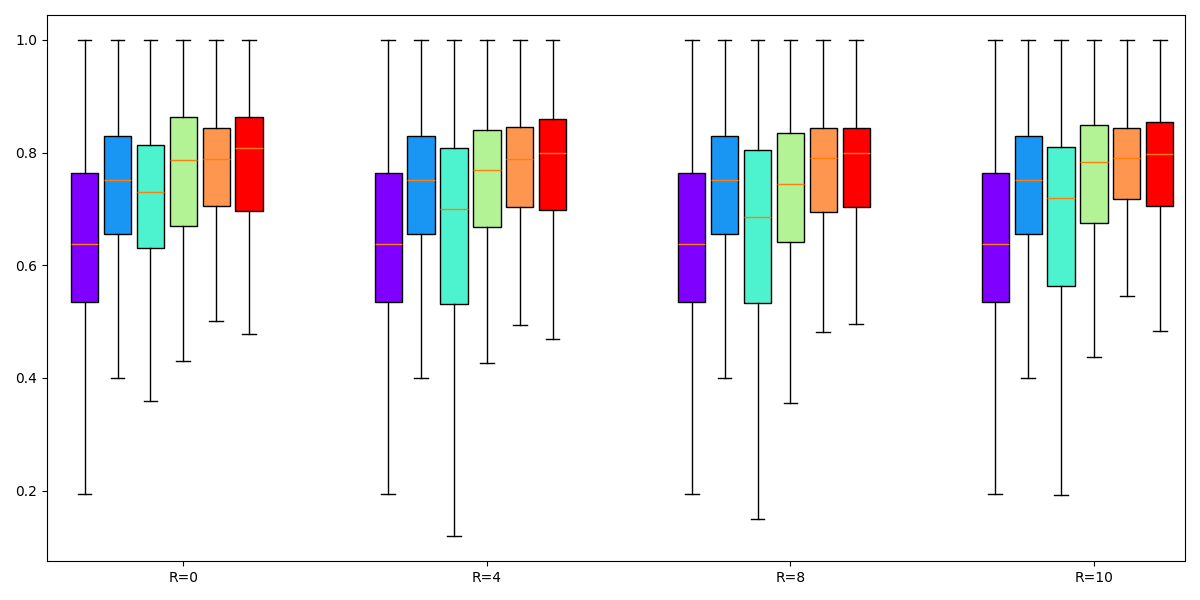
\includegraphics[width=\textwidth]{Boxplot_DiceScores_LV-Cavity.png}
    		\caption{Boxplot of the Dice scores for the left ventricle cavity.} %on the fully sampled \emph{ACDC} test data
    		\label{fig:Boxplot_DiceScores_LV-Cavity}
	\end{subfigure}
	\\
	\begin{subfigure}{0.8\textwidth}
    		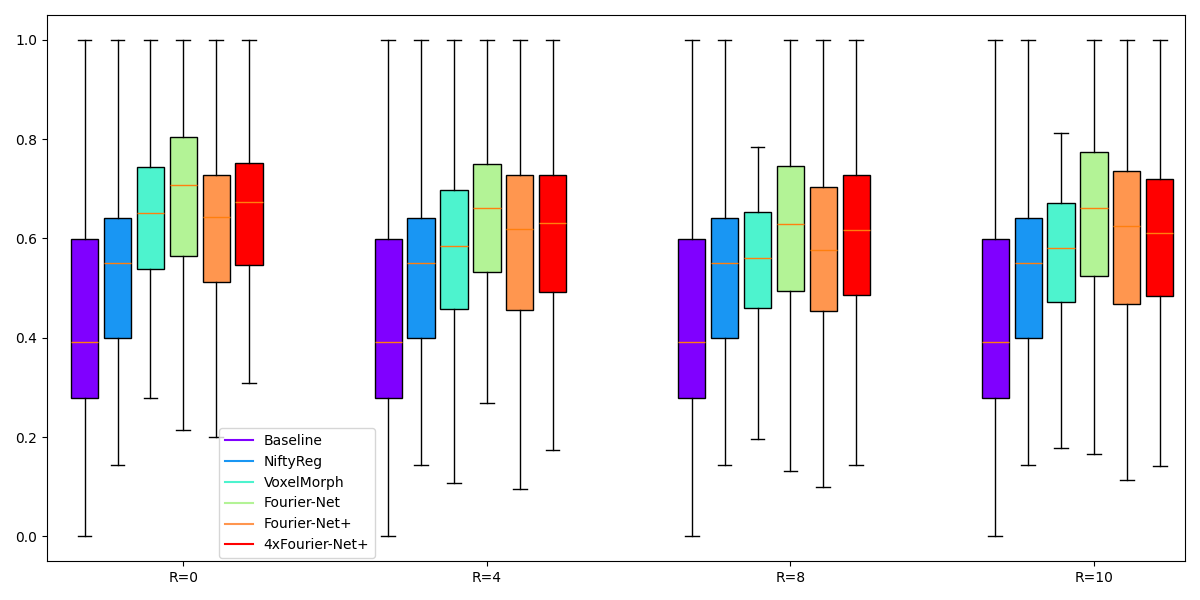
\includegraphics[width=\textwidth]{Boxplot_DiceScores_Myocardium.png}
    		\caption{Boxplot of the Dice scores for the myocardium.} %on the Acc4 \emph{ACDC} test data
    		\label{fig:Boxplot_DiceScores_Myocardium}
	\end{subfigure}
	\\
	\begin{subfigure}{0.8\textwidth}
    		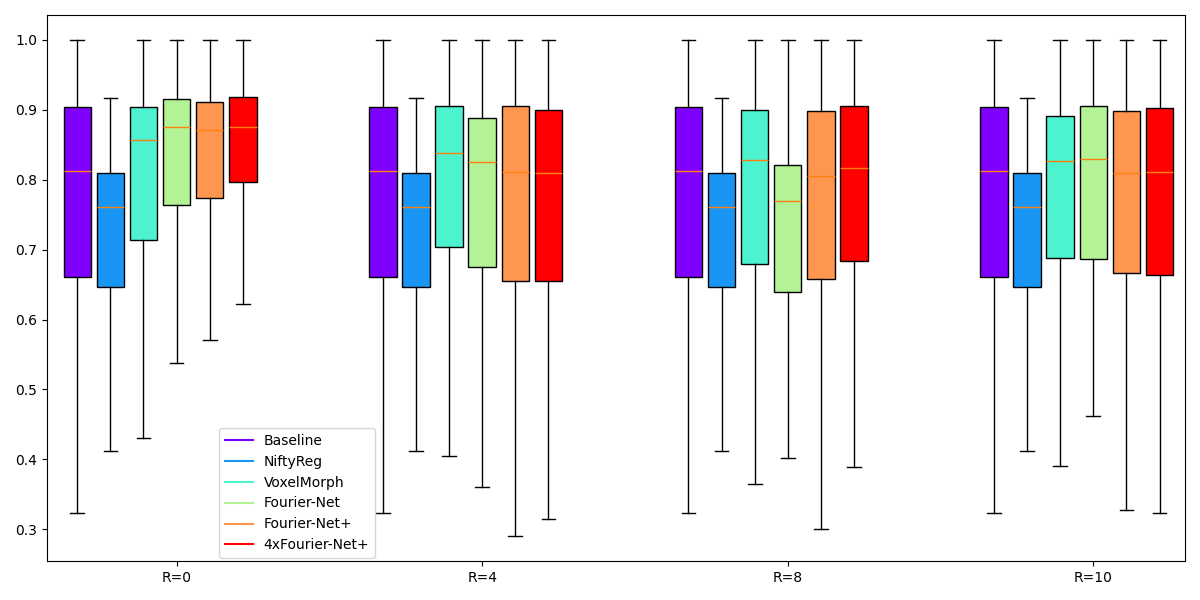
\includegraphics[width=\textwidth]{Boxplot_DiceScores_RV-Cavity.png}
    		\caption{Boxplot of the Dice scores for right ventricle cavity.} %on the Acc8 \emph{ACDC} test data
    		\label{fig:Boxplot_DiceScores_RV-Cavity}
	\end{subfigure}
	\caption{Boxplots of Dice scores (split by label excluding the background) for all models on fully sampled ($R=0$), Acc4 ($R=4$), Acc8 ($R=8$) and Acc10 ($R=10$) \emph{ACDC} test data.}
	\label{fig:Boxplots_DiceScores}
\end{figure}

%\begin{figure}[htpb]
%	\centering
%	\graphicspath{{images/}{\main/images/}}
%	\begin{subfigure}{\textwidth}
%    		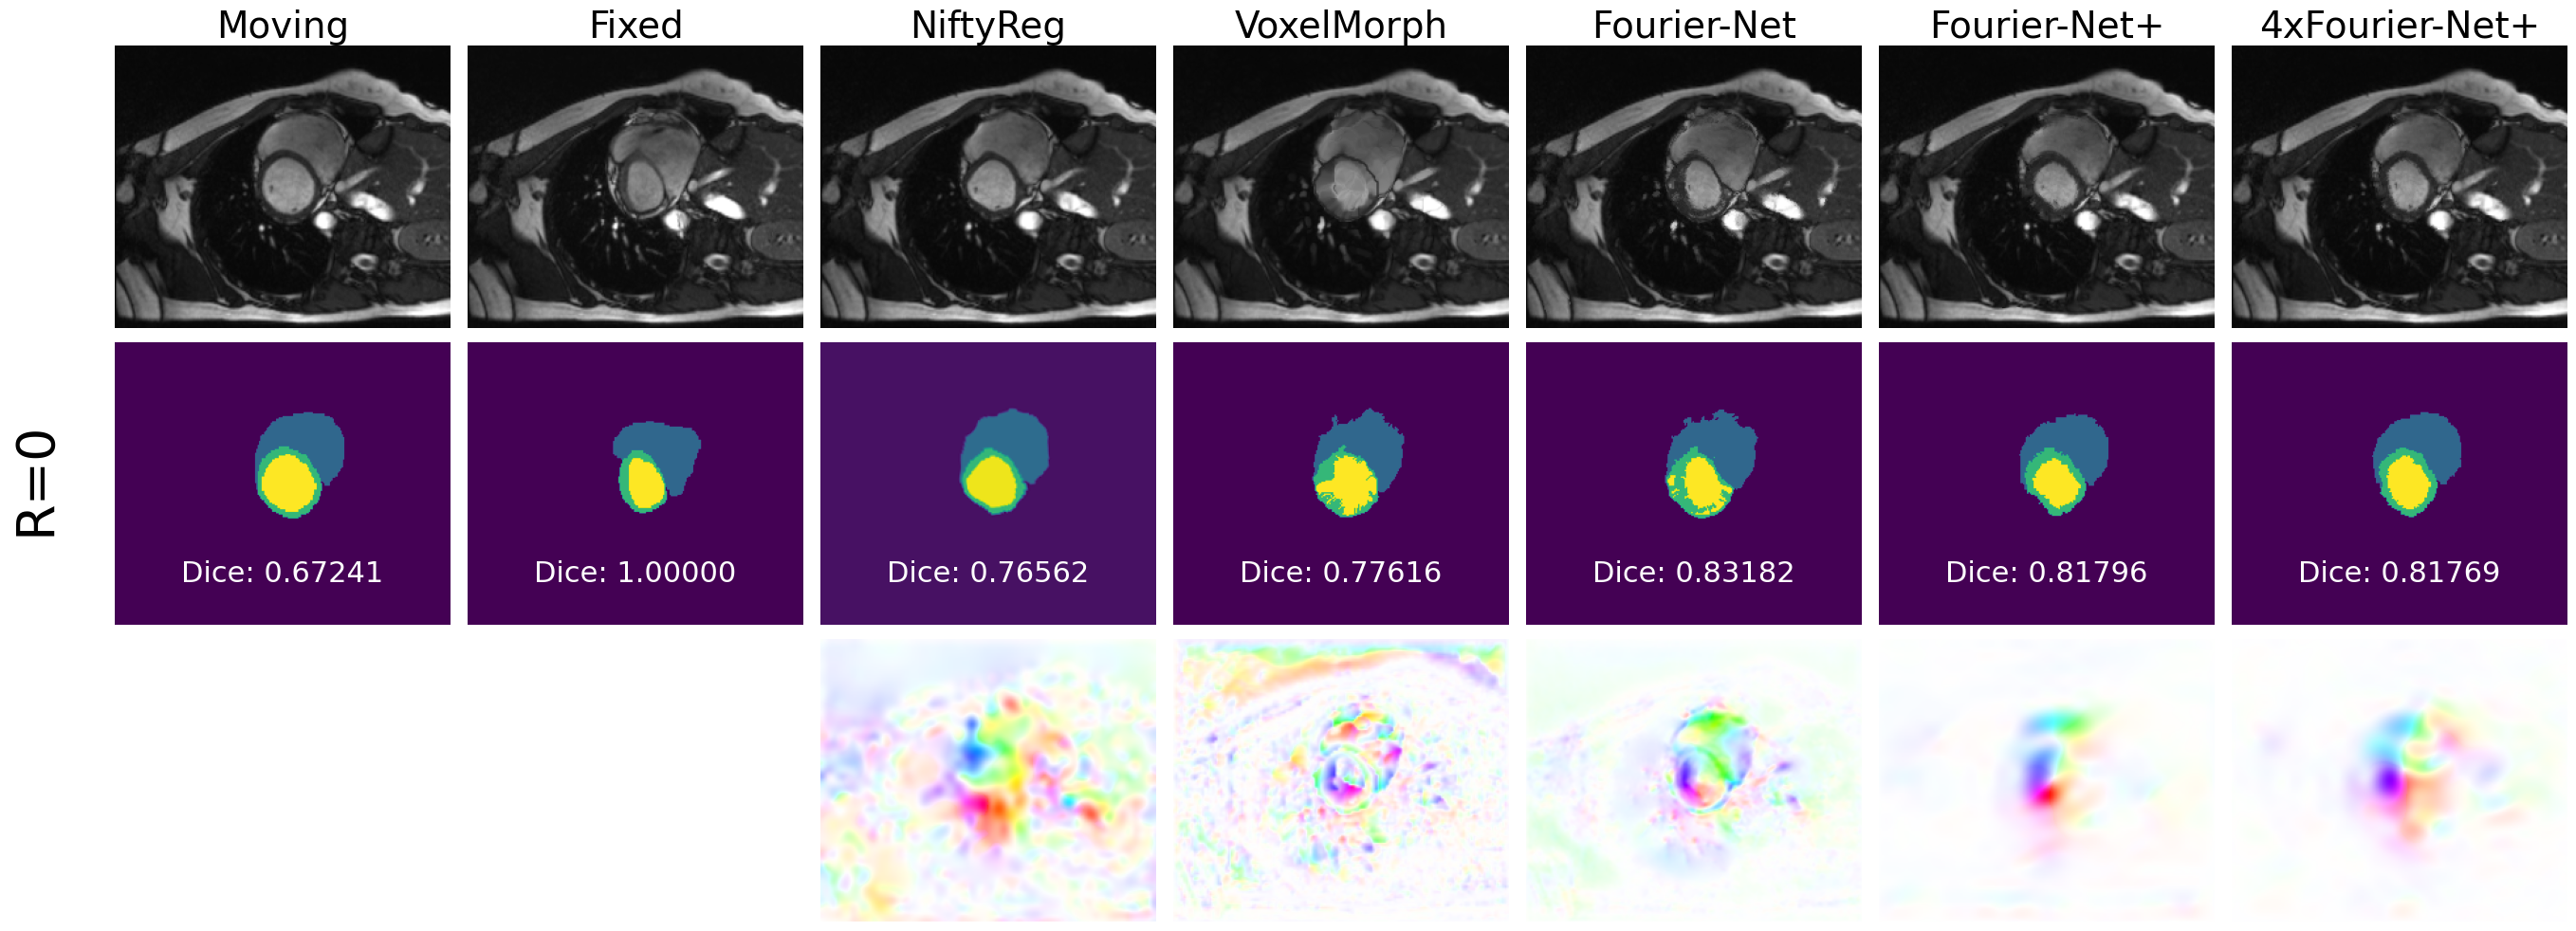
\includegraphics[width=\textwidth]{TestExamples_Mode0.png}
%    		\caption{Example images and segmentations for fully sampled ($R=0$) data.}
%    		\label{fig:TestExamples_Mode0}
%	\end{subfigure}
%	\\
%	\begin{subfigure}{\textwidth}
%    		\includegraphics[width=\textwidth]{TestExamples_Mode1.png}
%    		\caption{Example images and segmentations for Acc4 ($R=4$) data.}
%    		\label{fig:TestExamples_Mode1}
%	\end{subfigure}
%	\\
%	\begin{subfigure}{\textwidth}
%    		\includegraphics[width=\textwidth]{TestExamples_Mode2.png}
%    		\caption{Example images and segmentations for Acc8 ($R=8$) data.}
%    		\label{fig:TestExamples_Mode2}
%	\end{subfigure}
%	\\
%	\begin{subfigure}{\textwidth}
%    		\includegraphics[width=\textwidth]{TestExamples_Mode3.png}
%    		\caption{Example images and segmentations for Acc10 ($R=10$) data.}
%    		\label{fig:TestExamples_Mode3}
%	\end{subfigure}
%	\caption{Examples of warped images and segmentations for \emph{NiftiReg}, \emph{VoxelMorph}, \emph{Fourier-Net}, \emph{Fourier-Net+} and \emph{4xFourier-Net+} together with the original image pair from the \emph{ACDC} test data.}
%	\label{fig:TestExamples}
%\end{figure}

\begin{figure}[htpb]
	\centering
	\graphicspath{{images/}{\main/images/}}
	\includegraphics[width=\textwidth]{TestExamples_Mode0.png}
    	\includegraphics[width=\textwidth]{TestExamples_Mode1.png}
    	\includegraphics[width=\textwidth]{TestExamples_Mode2.png}
    	\includegraphics[width=\textwidth]{TestExamples_Mode3.png}	
	\caption{Examples of warped images, segmentations and flow fields for \emph{NiftiReg}, \emph{VoxelMorph}, \emph{Fourier-Net}, \emph{Fourier-Net+} and \emph{4xFourier-Net+} together with the original image pair from the fully sampled ($R=0$), Acc4 ($R=4$), Acc8 ($R=8$) and Acc10 ($R=10$) \emph{ACDC} test data.}
	\label{fig:TestExamples}
\end{figure}

% Too small!!!

%\begin{figure}[h] %tpb
%	\centering
%	\graphicspath{{images/}{\main/images/}}
%	\begin{subfigure}{0.5\textwidth}
%    		\includegraphics[width=\textwidth]{Boxplot_DiceScores_FullySampled.png}
%    		\caption{Boxplot of the Dice scores for $R=0$.} %on the fully sampled \emph{ACDC} test data
%    		\label{fig:}
%	\end{subfigure}
%	\\
%	\begin{subfigure}{0.5\textwidth}
%    		\includegraphics[width=\textwidth]{Boxplot_DiceScores_Acc4.png}
%    		\caption{Boxplot of the Dice scores for $R=4$.} %on the Acc4 \emph{ACDC} test data
%    		\label{fig:Boxplot_DiceScores_Acc4}
%	\end{subfigure}
%	\\
%	\begin{subfigure}{0.5\textwidth}
%    		\includegraphics[width=\textwidth]{Boxplot_DiceScores_Acc8.png}
%    		\caption{Boxplot of the Dice scores for $R=8$.} %on the Acc8 \emph{ACDC} test data
%    		\label{fig:Boxplot_DiceScores_Acc8}
%	\end{subfigure}
%	\\
%	\begin{subfigure}{0.5\textwidth}
%    		\includegraphics[width=\textwidth]{Boxplot_DiceScores_Acc10.png}
%    		\caption{Boxplot of the Dice scores for $R=10$.} %on the Acc10 \emph{ACDC} test data
%    		\label{fig:Boxplot_DiceScores_Acc10}
%	\end{subfigure}
%	\caption{Boxplots of Dice scores (split by label excluding the background) for all models on the \emph{ACDC} test data.}
%	\label{fig:Boxplots_DiceScores}
%\end{figure}


%\begin{figure}[h] %tpb
%	\centering
%	\graphicspath{{images/}{\main/images/}}
%	\includegraphics[width=\linewidth]{Boxplot_DiceScores_FullySampled.png} 
%	\caption{Boxplot of the Dice scores for all models sorted by label (excluding the background) on the fully sampled \emph{ACDC} test data.}
%	\label{fig:Boxplot_DiceScores}
%\end{figure}


%%%%%%%%%%%%%%%%%%%%%%%
%%%%%  Conclusion %%%%%
%%%%%%%%%%%%%%%%%%%%%%%

\chapter{Conclusion} \label{Ch:Conclusion}
Summery of all stuff...

\end{document}
